% !TeX spellcheck = uk_UA
\documentclass[14pt,twoside]{vakthesis}

\usepackage[T2A]{fontenc}
\usepackage[utf8]{inputenc}
\usepackage{cmap}%allows cyrillic search in pdf
\usepackage[english,russian,ukrainian]{babel}

\usepackage[intlimits]{amsmath}
\allowdisplaybreaks
\usepackage{amsthm}
\usepackage{amssymb, amsfonts}
\usepackage{enumerate,enumitem}
\usepackage{autonum}%нумерует только цитированные формулы
%\usepackage{hyperref}
\usepackage{tabularx, multirow}
\usepackage{graphicx,caption,subcaption}
\captionsetup{labelsep=period}
%\usepackage[export]{adjustbox}%for frames
\usepackage{wrapfig}
\usepackage{overpic,tikz}
\usetikzlibrary{calc}
\graphicspath{{images/}}
\usepackage{threeparttable,tablefootnote}
\usepackage{cite}
\usepackage{ulem}[normalem]

\usepackage{xcolor}
\definecolor{violet}{rgb}{0,0,0}
%\definecolor{red}{rgb}{0,0,0}
\usepackage{import}

%\usepackage{multibib}%multiple bibliograpphies
%% The new list's label is "New" and will be titled "The other list".
%% To put cites into this list, use \citeNew.
%\newcites{New}{The other list}


\usepackage{geometry}
\geometry{
	hmargin={30mm,10mm},
	vmargin={20mm,20mm},
	headsep=4mm
}

\newcommand{\colrr}{\color{red}}
\newcommand{\colb}{\color{blue}}
\newcommand{\colr}{\color{black}}
\newcommand{\colv}{\color{violet}}

\begin{document}

\institution{МІНІСТЕРСТВО ОСВІТИ І НАУКИ УКРАЇНИ\\ОДЕСЬКИЙ НАЦІОНАЛЬНИЙ УНІВЕРСИТЕТ імені І.І.МЕЧНИКОВА}{Одеса}

\author{СЕМЕНОВ АНДРІЙ КОСТЯНТИНОВИЧ}

\udc{538.956, 537.9, 544.72.05, 544.77}

\title{ЕЛЕКТРОФІЗИЧНІ ВЛАСТИВОСТІ\\
БАГАТОФАЗНИХ ДИСПЕРСНИХ СИСТЕМ}

\speciality[теоретична фізика\\Природничі науки]{01.04.02}[фізико-математичних наук]

\supervisor{Сушко Мирослав Ярославович}
           {кандидат фізико-математичних наук, доцент}

\date{\the\year}

\maketitle

\shipout\null
%%%%%%%%%%%%%%%%%%%%%%%%%%%%%%%%%%%%%%%%%%%%%%%
%\chapter*{Аннотація}
\import{./}{abstract_ua-utf8}

%\newpage
%\import{/}{abstract_ru}

\newpage
\import{./}{abstract_en-utf8}
%%%%%%%%%%%%%%%%%%%%%%%%%%%%%%%%%%%%%%%%%%%%%%%

%%%%%%%%%%%%%%%%%%%%%%%%%%%%%%%%%%%%%%%%%%%%%%%
%\begin{bibset}[*]{Список публікацій здобувача}
\newpage
\begin{center}
    {\normalfont \textbf{СПИСОК ПУБЛІКАЦІЙ ЗДОБУВАЧА}}
\end{center}
%%%%%%%%%%%%%%%%%%%%%%%%%%%%%%%%%%%%%%%%%%%%%%%
\vskip 20pt

%\begin{thebibliography}{1}
\import{./}{thesis_publications-utf8}
%\end{thebibliography}

%\end{bibset}

\newpage
%\addcontentsline{toc}{chapter}{Зміст}
\tableofcontents

%%%%%%%%%%%%%%%%%%%%%%%%%%%%%%%%%%%%%%%%%%%%%%%
\chapter*{Список основних скорочень та позначень}
%%%%%%%%%%%%%%%%%%%%%%%%%%%%%%%%%%%%%%%%%%%%%%%

\begin{itemize}
	\item[АМБ --] асиметрична модель Бруггемана
	\item[МКГ --] метод компактних груп
	\item[ПКЕ --] полімерні композитні електроліти
	\item[СМБ --] симетрична модель Бруггемана
%	\item[МГ --] Максвелл-Гарнетт
	\item[ТКЕ --] тверді композитні електроліти
	\item[RRN --] Random Resistor Network
	\item[SPFT --] Strong-property-fluctuation theory
	
	\item[$c$ --] об'ємна концентрація твердих ядер частинок
	\item[$c_{\rm c}$ --] положення порогу перколяції  через об'ємну концентрацію ядер
	\item[$d$, $R_1$ --] діаметр та радіус ядра
	\item[$h$ --] товщина оболонки
	\item[$s,t$ --] критичні індекси провідності в околі $c_{\rm c}$
	\item[$u$ --] відносна відстань до заданої точки від поверхні ядра розглядуваної частинки: $u=(r-R_1)/R_1$
	\item[$x$ --] $\sigma$, обезрозмірена на провідність ядра $\sigma_1$: $x=\sigma/\sigma_1$
	\item[$y$ --] $\varepsilon$, обезрозмірена на проникність ядра $\varepsilon_1$: $y=\varepsilon/\varepsilon_1$
	\item[${z}$ --] $\sigma$, обезрозмірена на провідність реальної матриці $\sigma_0$: ${z}=\sigma/\sigma_0$
	
	\item[$\delta$, $\delta_M$ --] відношення товщини оболонки $t$ до радіуса ядра $R_1$
	\item[$\delta\hat{\varepsilon}({\bf r})$ --] локальне відхилення комплексної діелектричної проникності від $\hat{\varepsilon}_{\rm f}$ спричинене компактною групою в точці $\bf r$ 
%	\item[$\delta(r)$ --] дельта-функція Дірака
	\item[$\varepsilon$ --] дійсна частина комплексної діелектричної проникності
	\item[$\hat{\varepsilon}_{\rm eff}$ --] ефективна комплексна діелектрична проникність
	\item[$\hat{\varepsilon}_{\rm f}$ --] комплексна діелектрична проникність матриці ${\cal M}$ допоміжної системи~$\cal S$
%	\item[$\theta(r)$ --] ступінчата функція Хевісайда
	\item[$\sigma$ --] квазістатична електрична провідність
	\item[$\phi$ --] об'ємна концентрація ядер разом з оболонками
%	\item[$\omega$ --] циклічна частота тестуючого поля
\end{itemize}


%%%%%%%%%%%%%%%%%%%%%%%%%%%%%%%%%%%%%%%%%%%%%%%
\chapter*{Вступ}
%%%%%%%%%%%%%%%%%%%%%%%%%%%%%%%%%%%%%%%%%%%%%%%

\import{./}{thesis_intro-utf8}


%%%%%%%%%%%%%%%%%%%%%%%%%%%%%%%%%%%%%%%%%%%%%%%
\chapter{Теоретичні методи дослідження ефективних електрофізичних властивостей невпорядкованих гетерогенних систем}\label{sec:overview}
%%%%%%%%%%%%%%%%%%%%%%%%%%%%%%%%%%%%%%%%%%%%%%%

Створення гетерогенних систем з наперед заданими ефективними електрофізичними властивостями (діелектричною проникністю $\varepsilon_{\rm eff}$ та електричною провідністю $\sigma_{\rm eff}$) є однією з нагальних задач сучасного матеріалознавства та виробництва.
Одними з найбільш поширених, але найменш теоретично досліджених є макроскопічно однорідні та ізотропні тривимірні гетерогенні системи, утворені диспергуванням частинок наповнювача в насучу матрицю. 
Вивчення ефективних характеристик таких систем потребує врахування не тільки багаточастинкових поляризаційних і кореляційних ефектів, що вже є дуже нетривіальною задачею, але й формування міжфазних шарів (областей просторового заряду в твердих композитних електролітах \cite{Dudney1988, NanC.-W.1991}; областей аморфізованого полімеру в полімерних композитних електролітах \cite{Przl1995,Wiec1994}; оксидних шарів в системах типу ізолятор--провідник \cite{Grannan1981,ChenI.-G.1986}; подвійних електричних шарів в коллоїдах та нанорідинах \cite{sarojini2013,Ohshima1982} тощо) та зміни електричних властивостей матриці (внаслідок неконтрольованого легування, забруднення, зміни внутрішньої структури тощо).

В даному розділі наведено огляд основних підходів, які використовуються для дослідження ефективних електрофізичних властивостей таких систем: класичні підходи Макс\-велла-Гарнетта та Бруггемана; методи знаходження меж допустимих значень ефективних параметрів; методи дослідження перколяційних ефектів; модельні системи частинок з морфологією ядро~-~оболонка, як спосіб врахування фізико-хімічних ефектів у системі; теорія SPFT (strong-property-fluctuation theory) для сильно неоднорідного середовища; та метод компактних групп неоднорідностей (МКГ), який кладеться за основу подальших досліджень.
Способи урахування міжфазних процесів коротко висвітлюються в підрозділі \ref{sec:core-shell-intro}, але основна увага їм приділена в подальших розділах.

Для опису суті методів та демонстрації основних співвідношень буде розглядатися статистично однорідна та ізотропна тривимірна двофазна немагнітна система ${\cal D}_0$, що складається з $N$ твердих сферичних частинок вкраплених в однорідне неперервне середовище (матрицю).
У даному розділі й надалі для розрахунків буде використовуватись система СГС(Е). 


\section{Класичні підходи Максвелла-Гарнетта та Бруггемана}\label{sec:Bruggeman}

Перші спроби опису ефективних електрофізичних властивостей багатофазних дисперсних систем до появи теорії електромагнетизму зводились до використання емпіричних співвідношень та феноменологічних міркувань для того чи іншого типу систем \cite{Priou}.
Наприклад, Гледстоун та Дейл \cite{Gladstone1863} вивчаючи заломлення світла в рідинах запропонували розглядати ефективну діелектричну проникність суміші як зважене середнє діелектричних проникностей її компонентів. Для двокомпонентної системи ${\cal D}_0$, що складається з частинок з діелектричною проникністю $\varepsilon_1$, вкраплених в несуче середовище (матрицю) проникністю $\varepsilon_0$, ефективна діелектрична проникність $\varepsilon_{\rm eff}$ в такому наближенні має вигляд
$$
\varepsilon_{\rm eff} = (1-c) \varepsilon_0 + c \varepsilon_1,
$$
де $c$ -- об'ємна концентрація частинок.
Іншим добре відомим емпіричним підходом, який узагальнює підхід Глед\-стоуна та Дейла, є підхід Ліхтенекера \cite{Licht1926, Goncharenko2000}:
\begin{equation}\label{eq:licht-k}
\varepsilon_{\rm eff}^k = (1-c) \varepsilon_0^k + c \varepsilon_1^k,
\end{equation}
де значення параметра $k$ належить проміжку $[-1,1]$; при $k=0$ вважається, що це рівняння набирає класичної логарифмічної форми \cite{Licht1926, Simpkin2010}:
\begin{equation}\label{eq:licht-ln}
\ln \varepsilon_{\rm eff} = (1-c) \ln \varepsilon_0 + c \ln \varepsilon_1.
\end{equation}
В чисельних роботах \cite{Sheng, BergmanB, Sihvola1999, Brosseau2003} показано, що такі підходи можуть бути використані для інтерполяції окремих типів систем, але не можуть бути узагальнені для отримання більш точних результатів. Більш докладний історичний огляд цих підходів можна знайти, наприклад, в \cite{Brosseau2006}.

Перші кроки до послідовного аналітичного опису електрофізичних властивостей гетерогенних систем були зроблені Максвеллом у другій половині 19-го століття при побудові фундаменту теорії електромагнітизму.
В роботі \cite{Maxwell1892} він розглянув задачу знаходження електростатичної провідності невпорядкованої тривимірної двокомпонентної системи, що складається з металевих кульок провідністю $\sigma_1$, вкраплених в несуче середовище (матрицю) провідністю $\sigma_0$ так, що електричною взаємодією кульок між собою та з поверхнею системи можна знехтувати. 
Для цього спочатку розв'язувалась задача знаходження електростатичної провідності системи, що складалась з однієї маленької кульки провідністю $\sigma_1$ всередині великої кулі провідністю $\sigma_0$. Провідність такої системи знаходилась з умов неперервності електростатичного потенціалу та електричного струму на поверхні розділу куль. Далі, вважаючи, що всередині великої кулі знаходяться багато малих незалежних одна від одної кульок, з оцінки асимптотичної поведінки поля такої системи на далекій відстані від цих кульок  було знайдено наступне співвідношення для ефективної провідності $\sigma_{\rm eff}$  системи:
\begin{equation}\label{eq:MG}
\frac{\sigma_{\rm eff} - \sigma_0}{2\sigma_0 + \sigma_{\rm eff}} = c \frac{\sigma_1 - \sigma_0}{2\sigma_0 + \sigma_1},
\end{equation}
де $c$ -- об'ємна концентрація малих кульок в системі. 
В роботі Релея \cite{Rayleigh}, де вивчалась провідність періодично розподілених куль в матриці, показано, що підхід Максвелла є добрим першим наближенням до опису $\sigma_{\rm eff}$ таких систем та враховує тільки дипольні внески.
Пізніше Максвеллом-Гарнеттом  \cite{M-G1904} була розглянута задача поширення електромагнітної хвилі крізь систему металевих кульок для вивчення коефіцієнта заломлення світла. Для врахування взаємної поляризації частинок вважалось, що кожна знаходиться в так званому полі Лорентца \cite{Lorentz1870, Choy}, яке складається із внесків зовнішнього поля та поля інших частинок. В рамках поняття поля Лорентца останній внесок еквівалентний поляризаційному внеску деякої сфери (сфери Лорентца), що має розміри порядку масштабу усереднення \cite{Choy}, всередині якої знаходиться розглядувана частинка. 
Це поняття робить розгляд системи еквівалентним розглянутому вище методу Максвелла, де кожна частинка також розглядалась окремо всередині великої кулі.
Для систем з діелектричними компонентами ефективну діелектричну проникність $\varepsilon_{\rm eff}$ в рамках такого підходу можна знайти, обчисливши дипольний момент одиниці об'єму гетерогенної системи як суму дипольних моментів окремих частинок в полі Лорентца, виражених через діелектричні проникності частинок і матриці.
Наприклад, для системи діелектричних куль з проникністю $\varepsilon_1$, хаотично розподілених в матриці проникністю $\varepsilon_0$, співвідношення для знаходження $\varepsilon_{\rm eff}$ має вигляд, аналогічний (\ref{eq:MG}) \cite{Markel2016,Choy}.

Узагальнення підходу Максвелла-Гарнетта (МГ) на системи з комплексними  проникностями відоме як підхід Максвела-Вагнера-Сілларса~\cite{Wagner1914, Sillars1937}.

Одним з головних недоліків підходу МГ є те, що він є по суті одночастинковим наближенням, яке може використовуватись лише коли
наближення поля Лорентца є виправданим, тобто коли локальне електричне поле навколо кожної частинки в межах сфери Лорентца з достатньою точністю можна розглядати окремо від інших частинок і вважати цю область однорідно поляризованою. Це твердження підтверджується нефізичними результатами, до яких призводить цей підхід при достатньо великих концентраціях включень. Наприклад, для багатофазних систем в рамках підходу МГ при концентраціях включень, коли вся система зайнята лише дисперсною фазою, ефективні характеристики ще будуть залежати від характеристик матриці, фаза якої вже відсутня в системі. Якщо йде мова про системи еліпсоїдальних частинок при великих концентраціях дисперсної фази, підхід МГ також дає нефізичні результати \cite{Choy}.
Різноманітні узагальнення та поліпшення цього підходу можна 
знайти в~\cite{Sihvola2000}. 

Наступним істотним кроком у вивченні розглядуваних систем був їх аналіз в рамках моделі ефективного середовища \cite{Biot1806}. Для аналізу ефективних електрофізичних параметрів цей підхід для багатофазних дисперсних систем було вперше запропоновано Бруггеманом \cite{Bruggeman1935}. В рамках підходу Бруггемана частинки кожного з компонентів  системи (включаючи гранули матриці) розглядаються окремо, як усамітнені частинки, що знаходиться в середовищі з проникністю $\varepsilon_{\rm eff}$ (провідністю $\sigma_{\rm eff}$), значення якої формується всіма компонентами системи.
Це припущення передбачає, що локальне електромагнітне поле є однаковим для кожного з компонентів системи, не збурене присутністю інших компонентів та еквівалентне полю в середовищі з проникністю $\varepsilon_{\rm eff}$ (провідністю $\sigma_{\rm eff}$).
Співвідношення для $\varepsilon_{\rm eff}$ для  системи ${\cal D}_0$ діелектричних куль в діелектричній матриці в рамках такого підходу можна отримати з умови, що загальний дипольний момент частинок компонентів системи в ефективному середовищі дорівнює нулю, а тому додавання нових частинок компонентів в ефективне середовище не змінює це значення \cite{Ross2004, Bruggeman1935, Landauer1952, Ross2004, Torquato}:
\begin{equation}\label{eq:EMA}
(1-c) \frac{\varepsilon_0 - \varepsilon_{\rm eff}}{2\varepsilon_{\rm
		eff} + \varepsilon_0} + c \frac{\varepsilon_1 -
	\varepsilon_{\rm eff}}{2\varepsilon_{\rm eff} + \varepsilon_1} = 0.
\end{equation}
Аналогічне співвідношення можна знайти для ефективної провідності $\sigma_{\rm eff}$ двокомпонентної системи, вважаючи рівними струми, що проходять крізь неоднорідну та гомогенізовану системи, та ефективні провідності останніх \cite{Landauer1952, Torquato}.
Підхід Бруггемана можна узагальнити на багатофазні системи несферичних та анізотропних за своїми властивостями частинок з комплексними проникностями або провідностями компонентів, застосовувати до опису інших ефективних характеристик дисперсних систем тощо \cite{Choy, Sihvola1999, Torquato, Mackay}. 

Незважаючи на те, що класичний підхід Бруггемана та його припущення слугують базою для ряду підходів, розроблених для специфічних типів систем, які досі застосовуються та розвиваються~\cite{Choy,Stroud1998,Milton,Banheg1986}, він має декілька істотних недоліків.
По-перше, за побудовою класичний підхід Бруггемана враховує поляризаційні та кореляційні взаємодії розглядуваної частинки з всіма іншими компонентами лише через електрично однорідне ефективне середовище, властивості якого формуються цими компонентами незалежно від їх відстані до заданої частинки. Тому цей підхід по суті є одночастинковим, його застосовність при великих концентраціях видається проблематичною, хоча на практиці він та його модифікації успішно використовуються й для більш високих концентрацій для окремих класів систем (див. наприклад \cite{Wiec1994, Zhou2012, McLachlan1990}).
По-друге, в рамках класичного підходу Бруггемана фаза матриці розглядається, як сукупність частинок, які мають таку ж саму геометричну форму, як і частинки дисперсної фази. Таке твердження не є фізично виправданим~\cite{Chelidze} та дає, наприклад для еліпсоїдальних частинок, нефізичні результати~\cite{Brouers1986,Kirkpatrick1971,Torquato}.
Обговорення цих та інших недоліків та границь застосування підходу Бругемана можна знайти в~\cite{Torquato,Choy,Sihvola1999,Brosseau2006,Milton}.

Підхід ефективного середовища Бруггемана ще називають симетричною моделлю Бруггемана (СМБ). В рамках симетричних моделей кожен з компонентів (матриця та частинки дисперсної фази) розглядаються аналогічно, зокрема, як сферичні частинки в ефективному середовищі. Прикладом асиметричного підходу є підхід МГ, де кожна частинка дисперсної фази розглядається окремо на фоні певної явно виділеної фази (матриці).
Ідею асиметричного моделювання системи можна реалізувати й в рамках підходу ефективного середовища (див. розділ \ref{sec:Hanai-analysis}).


\section{Межі допустимих значень ефективних характеристик}\label{sec:HS}

У ситуації, коли кількісний розрахунок  ефективних параметрів системи є задачею, далекою до остаточного розв'язання, та характеризується низкою неконтрольованих наближень, надзвичайної ваги набувають дослідження меж їх можливих значень.
Ці дослідження належать до так званої теорії гомогенизації~\cite{Torquato,Milton,Sihvola1999,Jikov}, в рамках  якої розглядаються аналітичні властивості рівнянь, що описують лінійний відгук окремих класів систем.
Чим більше інформації враховано про даний клас (мікроструктура, внутрішня симетрія, присутні процеси та механізми тощо), тим  більш точними вважаються отримані межі \cite{Cule1999,Torquato}.

Перші межі для двофазних систем були отримані Вінером \cite{Wiener1912}, який розглянув два граничних випадки  мікроструктури системи: 
(а) послідовно (по відношенню до зовнішнього поля ${\bf E}_0$) впорядковані пластини різної товщини, з провідностями $\sigma_1$ й $\sigma_2$ та об'ємними концентраціями $c_1$ та $c_2=1-c_1$; (б) ті ж самі пластини, але паралельно впорядковані. 
Розв'язуючи відповідні електростатичні задачі, можна знайти  ефективні провідності $\sigma_{\rm eff}$ цих систем, перша з яких відповідає нижній межі $\sigma^{-}$, а друга -- верхній $\sigma^{+}$:
\begin{equation}\label{eq:wiener-bounds}
\begin{split}
\sigma^{-} = \left( \frac{c_1}{\sigma_1} + \frac{c_2}{\sigma_2} \right)^{-1};\qquad
\sigma^{+} = c_1 \sigma_1 + c_2 \sigma_2.
\end{split}
\end{equation}
Таку  саму структуру мають межі для   $\varepsilon_{\rm eff}$.
Вони повинні справджуватися також для довільних двофазних систем з комплексними діелектричними проникностями \cite{Aspnes1982}.

Подальші дослідження в цій сфері були зосереджені на уточненні меж Вінера для різних конкретних симетрій та мікроструктур \cite{Torquato,Sihvola1999,Milton}. Для розглядуваних тривимірних двофазних макроскопічно однорідних та ізотропних гетерогенних систем найбільш жорсткими, що можуть бути записані через об'ємні концентрації та провідності (діелектричні проникності)  компонентів, є межі Хашина-Штрікмана:
\begin{equation}\label{eq:HS-bounds}
	\begin{split}
	\sigma^{-} = \sigma_1 + \frac{3c_2 \sigma_1(\sigma_2-\sigma_1)}{3\sigma_1 + c_1(\sigma_2-\sigma_1)};\qquad
	\sigma^{+} = \sigma_2 + \frac{3c_1 \sigma_2(\sigma_1-\sigma_2)}{3\sigma_2 + c_2(\sigma_1-\sigma_2)},
	\end{split}
\end{equation}
отримані в \cite{HS1962} на базі певних загальних варіаційних теорем.
Варіаційні теореми Хашина-Штрікмана \cite{HS1962} можуть бути використані й для узагальнення цих меж на багатофазні та анізотропні системи, системи з комплексними значеннями проникностей чи провідностей компонентів тощо \cite{Torquato,Milton,Sihvola1999}. 

Подальші спроби уточнення меж на допустимі значення ефективних параметрів здійснювалися в напрямі використання більш докладної інформації про мікроструктуру системи, ніж та, яку надає об'ємна концентрація компонентів.  Вони отримали назву "поліпшених меж" ("improved bounds") \cite{Torquato,Sihvola1999} і, за означенням, вони нетривіальним чином залежать від двоточкової та вищих кореляційних функцій. 

Для знаходження ``поліпшених'' меж користуються формальним розкладом $\sigma_{\rm eff}$ за ступенями величини $(\sigma_2-\sigma_1)/\sigma_1$ \cite{Torquato1991,Torquato}. Кожний доданок в цьому ітераційному ряді містить внески кореляційних функцій відповідного порядку. У першому та другому порядках за величиною $(\sigma_2-\sigma_1)/\sigma_1$ відтворюються відповідно межі Вінера та Хашина-Штрікмана, записані у тих же порядках. Поліпшені межі отримують розглядаючи члени ряду більш високих порядків.  Стверджується \cite{Torquato}, що чим більше багаточастинкових внесків враховано при розрахунках, тим більш вузькими будуть поліпшені межі. При цьому їх розрахунки ведуться лише числовими методами для обмеженої кількості модельних кореляційних функцій \cite{Cule1999}. 

Очевидно, що такий підхід застосовний лише для систем із відповідними значеннями провідностей компонентів, а тому виникає питання про їх застосовність до систем з великою різницею у значеннях провідностей. По-друге, для розрахунку поліпшених меж необхідно знати вигляд багаточастинкових кореляційних функцій, як правило невідомих. 
Через це, до використання ``поліпшених'' меж треба відноситись з обережністю. 
Наприклад, розглянута СМБ (\ref{eq:EMA}) задовольняє межі Хашина-Штрік\-мана (\ref{eq:HS-bounds}), але не задовольняє ``поліпшені'' межі \cite{Torquato} для систем із істотною різницею значень провідностей компонентів. З другого боку, порушення меж Хашина-Штрікмана вестиме до порушення і ``поліпшених'' меж. Цей факт використано в розділі \ref{sec:Hanai-analysis} для критичного аналізу диференціального методу та його модифікацій.

Істотні результати в напрямі отримання поліпшених меж були отримані Бергманом \cite{Bergman1978,Bergman1992}, Мільтоном \cite{Milton}, Торкуато \cite{Torquato1991,Torquato} та іншими авторами. Крім варіаційного принципу є ще низка інших підходів для отримання меж \cite{Milton,Torquato,Sihvola1999,Cioranescu,Jikov}, серед яких одними з найпотужніших є метод компенсованої компактності \cite{Tartar1979,Milton} та методи математичної теорії міри  \cite{Tartar1990}, які дали початок розвитку математичної теорії гомогенизації \cite{Cioranescu,Jikov}.


\section{Методи теорії перколяції}\label{sec:perc}
 
Ефект електричної перколяції проявляється зазвичай у вигляді різкої зміни ефективної провідності на вузьких концентраційних інтервалах в системах з істотними різницями між провідностями компонентів (системах типу ізолятор~-~провідник \cite{Grannan1981,ChenI.-G.1986}, системах на основі рідкокристалічної \cite{Tomylko2015, Lebovka2017} та полімерної \cite{Lebovka2011, Lysenkov2012, Klepko2015} матриць з додаванням нанотрубок тощо). 
Сам термін ``перколяція'' та математичне вивчення цього ефекту вперше з'явилися в роботі Бродбента і Хаммерслі у 1957 році~\cite{Broad57}. Після цієї роботи та фундаментальних робіт в сфері критичних явищ в фізиці теорія перколяції почала досить стрімко розвиватись та отримала сильну математичну базу \cite{BergmanB, Kirkpatrick1973, Aharony, Bollobas, Meester, Sahimi, Hunt} й широке застосування не тільки в фізиці \cite{Aharony,Sahimi2}. 

Ефект електричної перколяції виникає за рахунок формування більш провідними компонентами так званих перколяційних кластерів, які простягаються через всю систему та слугують шляхами протікання струму.
Концентрацію високопровідного компоненту $c_{\rm c}$, при якій існує ненульова ймовірність виникнення такого кластеру, називають порогом перколяції. В околі цієї точки провідність системи $\sigma_{\rm eff}$ на практиці інтерполюють степеневими законами:
\begin{equation}\label{eq:perc-indexes-s-t}
\sigma_{\rm eff} \sim \left\{ 
\begin{array}{ll}
(c_{\rm c} - c)^{-s}, & c< c_{\rm c},\\
(c - c_{\rm c})^t, & c> c_{\rm c},
\end{array}
\right.
\end{equation}
де $s$ і $t$ -- перколяційні критичні індекси провідності. За визначенням~\cite{Aharony,Torquato,Sahimi,Hunt}, індекс $t$ вводиться для систем з нульовою провідністю матриці, а індекс $s$ -- для систем з нульовим опором дисперсної фази; поріг перколяції $c_{\rm c}$ зазвичай визначають для систем з непровідною матрицею та провідними компонентами. Слід зазначити, що вже СМБ передбачає появу ефекту перколяції в провідних системах, але дає  значення розглядуваних характеристик ($s=t=1$, $c_{\rm c}=1/3$), які не підтверджується на числових симуляціях \cite{Kirkpatrick1973,Torquato,Aharony}. Причиною цього є те, що перколяція -- багаточастинковий ефект, для вивчення якого необхідно знати багаточастинкові кореляційні функції відповідної системи. Як вже зазначалось, для більшості систем такий підхід неможливий, тому перколяційні задачі зазвичай розглядають в рамках числових методів. Зокрема, для системи ${\cal D}_0$ твердих куль отримано наступні значення: $s\approx 0.73$, $t\approx 2$ \cite{Aharony}, $c_{\rm c} \approx 0.183$~\cite{Powel1979}.
Крім цього, окремою проблемою є зв'язок параметрів компонентів з параметрами теорії.

В рамках теорії перколяції індекси $s$, $t$ та поріг перколяції вважаються фіксованими для відповідного класу мікроструктури системи та залежать лише від розмірності простору (гіпотеза універсальності) \cite{Aharony,Torquato,Hunt}. 
Ця гіпотеза та вивчення систем в рамках теорії перколяції із залученням співвідношень типу (\ref{eq:perc-indexes-s-t}) дає можливість вивчати колективну поведінку великих класів  систем з різною мікроструктурою. 

На практиці результати застосування  скейлінгових співвідношень (\ref{eq:perc-indexes-s-t}) до реальних систем зі схожою мікроструктурою, але з різними матеріалами складових та/або різними способами виготовлення, суперечать гіпотезі універсальності. Наприклад, значення індексу $t$ може лежати у проміжку $1.5\div 2$~\cite{Nan1993}, і навіть мати й більші значення \cite{Balberg1987,Nan1993}; значення індексу $s$ зазвичай лежать у проміжку $0.7 \div$1.0 \cite{Nan1993}.
Положення порогу перколяції в таких системах також різняться. 
Однією із можливих причин може бути той факт, що в реальних системах вступають в дію різноманітні фізико-хімічні процеси як на межі розділу фаз, так і всередині окремих компонентів, які не враховуються двофазними моделями. 


\section{Модельні системи частинок з морфологією ядро~-~оболонка}\label{sec:core-shell-intro}

Міжфазні та матричні ефекти можуть істотним чином впливати на ефективні електрофізичні характеристики системи не лише в області порогу перколяції, але й на всьому концентраційному інтервалі.
Наприклад, відомо \cite{Maier1986, Nan1993}, що в твердих композитних електролітах, які складаються з непровідних частинок (наприклад, $\rm Al_2O_3$, $\rm TiO_2$ тощо), диспергованих в полікристалічній матриці галоїдів металів ($\rm LiI$, $\rm PbCl_2$ тощо), формуються, переважно в околі поверхні частинок, області просторового заряду, спричинені високою концентрацією  дефектів  матриці. Ці області мають питому провідність на кілька порядків більшу, ніж провідності окремих компонентів системи. При збільшенні концентрації дисперсної фази ефективна провідність зростає за рахунок зростання об'ємної частки цих високопровідних областей, які вже при досить невеликих концентраціях ($c\approx0.1$) можуть формувати перколяційні кластери. При деякій концентрації частинок провідність досягає максимального значення (яке може на кілька порядків перевищувати $\sigma_0$) та починає спадати з подальшим зростанням $c$, що пов'язано з блокуванням перколяційних шляхів непровідною дисперсною фазою. 
Аналогічна поведінка провідності спостерігається в полімерних композитних електролітах \cite{Wiec1994,nanocomp2008,sequera2010}, де в якості матриці виступають полімери (наприклад, поліетилен оксид, поліетилен-гліколь-метил), що можуть формувати електродонорні зв'язки з різними неорганічними солями (наприклад, $\rm LiClO_4$, $\rm NaI$); в якості дисперсної фази виступають непровідні неорганічні частинки (наприклад, $\rm \theta-Al_2O_3$, $\rm TiO_2$), або глобули полімеру іншого сорту (наприклад, поліакриламіду) \cite{nanocomp2008}. В цих системах навколо частинок дисперсної фази формуються області аморфізованого полімеру,  провідність яких знову ж таки вища за провідності окремих компонентів системи.
Іншими прикладами міжфазних ефектів можуть бути формування оксидних шарів на поверхні металевих частинок \cite{ChenI.-G.1986,Grannan1981}; формування подвійних електричних шарів в колоїдах \cite{Ohshima1982}); контактний опір; неоднорідність форм та розмірів частинок.

Крім міжфазних ефектів, на значення ефективної провідності систем типу композитних електролітів впливають й матричні ефекти: формування високопровідної мережі зв'язаних дислокацій, утворених механічним або термічним шляхом~\cite{Dudney1987, Dudney1988, Muhlherr1988}; швидкий іонний транспорт уздовж поверхні розділу матриця~-~частинки та/або дислокацій~\cite{Phipps1981, Atkinson1988}; однорідне легування матриці за рахунок розчинення неоднорідностей та малих частинок~\cite{Wen1983, Dupree1983, Dudney1985} тощо.

Традиційним методом врахування міжфазних ефектів в багаточастинкових системах є вивчення останніх в рамках модельної системи невпорядкованих сферичних частинок з морфологією ядро~-~оболонка \cite{Torquato, Choy}. В рамках цього методу частинки дисперсної фази моделюються у вигляді твердих (непроникних) куль, які покриті концентричними оболонками; останні можуть бути як тверді, так і проникні.
Найбільш розповсюдженою та вивченою є модель тверде ядро~-~тверда оболонка, яка зазвичай аналізується в рамках класичних підходів \cite{Choy,Sihvola1999}. Наприклад, узагальнюючи підхід МГ на випадок частинок з твердим міжфазним шаром, можна описати дані для діелектричної проникності композитів на основі епоксидної смоли з різними типами діелектричних включень \cite{Vo2002}. 
Модель тверде ядро~-~тверда оболонка також застосовується в теорії провідності колоїдних суспензій \cite{Ohshima1982,Lyklema1995}, як найпростіше припущення для побудови коміркової моделі \cite{Lyklema1995,Torquato}.
Однак, для опису багатьох інших ефектів моделі твердих оболонок виявляється недостатньо (див. наприклад \cite{Wiec1994,  Tomylko2015, Singh2018}). 

Модельні системи частинок з морфологією тверде ядро~-~проникна оболонка (soft shell model, cherry-pit model, inverse ``swiss-cheese'' model \cite{Torquato}) виявляються більш гнучкими.
Але на відміну від моделі тверде ядро~-~тверда оболонка, аналітичне вивчення цих моделей вже у випадку електрично однорідних оболонок набагато складніше. Зокрема, виникає питання, що вважати окремою частинкою: окремі ядра з їх оболонками, або кластери частинок з перекритими оболонками. Виникає необхідність розрахунку окремих багаточастинкових внесків, що є дуже складною задачею навіть у простому випадку сферичних частинок з повністю проникними оболонками \cite{Torquato}. 
Через це задачі вивчення впливу міжфазних ефектів в рамках моделі з проникними оболонками зазвичай розв'язується числовими методами (див. наприклад \cite{Myroshnychenko2008,Myroshnychenko2009}) або аналітично з використанням класичних моделей та низки емпіричних припущень.

Типовим прикладом таких аналітичних теорій є підхід Нана та Сміта~\cite{Nan1987, NanC.-W.1991, Nan1993} для вивчення $\sigma_{\rm eff}$ систем твердих композитних електролітів, що базується спрощеному емпіричному підході Накамури \cite{Nakamura1984}, що базується на досить грубих фізичних припущеннях.
Щоб обійти задачу розрахунку складних багаточастинкових внесків кластерів частинок, розглядається поведінка системи в наступних двох граничних випадках, розв'язки для яких зшиваються: 1) частинки з оболонкою вважаються ізольованими одна від одної, так що їх оболонки можна вважати твердими; 2) фаза матриці майже повністю витіснена міжфазним шаром. При цьому оболонки вважаються електрично однорідними. 
В першому випадку трьохфазна система матриця~-~ядро~-~оболонка моделюється як квазідвофазна: матриця~-~дисперсна фаза, де провідність дисперсної фази дорівнює ефективній провідності частинки з оболонкою~\cite{Maxwell1892, Brailsford1986, Chettiar2012}.
Максимум провідності досягається при  $c = c_{\rm max} = (1+\delta)^{-3}$, коли вся фаза матриці витіснена фазами ядер частинок та оболонок. 
Після цього (при $c > c_{\rm max}$) система розглядається, як сукупність твердих ядер частинок, які знаходяться в матриці, утвореній фазою оболонок. 

Базові припущення моделі Нана
дуже звужують клас систем, до яких застосовний підхід.
Зокрема, вони не дозволяють застосувати модель до систем полімерних композитних електролітів, де міжфазні оболонки мають електрично неоднорідний профіль провідності \cite{nanocomp2008}.
Для того щоб обійти ці труднощі, Вічореком та колегами~\cite{Wiec1989,Wiec1994,Przl1995} було запропоновано    ввести залежність відносної товщини оболонки $\delta$ від концентрації частинок $c$ у вигляді підгонного поліному другого порядку. 

В рамках моделі тверде ядро~-~проникна оболонка можна також описати ефект подвійної перколяції в двовимірних рідкокристалічних системах з диспергованими нанотрубками \cite{Tomylko2015, Lebovka2017}, де в якості ядер виступають компактні провідні агрегати сплутаних нанотрубок, а в якості  менш провідних проникних оболонок -- області навколо цих агрегатів з меншою щільністю, або сольватаційні оболонки \cite{Lebovka2017}; релаксаційні процеси в двовимірних системах стрижнів \cite{Lebovka2019}, де проникні оболонки можна використовувати для моделювання взаємодії між стрижнями; немонотонну поведінку ефективної провідності полімерних композитних електролітів з електрично неоднорідними радіально-симетричними проникними оболонками \cite{nanocomp2008} тощо. 

Таким чином моделі систем частинок з морфологією тверде ядро~-~проникна оболонка дозволяють ефективно описувати різні фізико-хімічні ефекти, але їх аналітична реалізація вимагає подальших розробок. Це і є однією із задач дисертаційної роботи.


\section{Теорія SPFT}\label{sec:SPFT}

Гетерогенну багаточастинкову систему можна розглядати як середовище із сильно флуктуюючими локальними значеннями його властивостей. Розгляд такої моделі в рамках задачі поширення електромагнітних хвиль в середовищі вперше запропонував Лішфиць з колегами \cite{Lifshitz1950}. Пізніше цей підхід розвивався Бюрре~\cite{Bourret1962}, Рижовим, Тамойкіним та Татарським~\cite{Ryzhov1965,
RyzhovRev}, Цангом~\cite{Tsang1981}, Жуком~\cite{Zhuk1994} та іншими авторами.
Остаточне формулювання ця теорія, за якою закріпилася назва  strong-propertyfluctuation
theory (SPFT), отримала в роботах Маккея, Лакхтакії та Вейкгофера~\cite{Michel1995,Mackay2000, Mackay2001}.
Останні автори, посилаючись на результати~\cite{Tsang1981}, які в свою чергу спираються на результати~\cite{Ryzhov1965, RyzhovRev}, узагальнили  теорію і на задачі про знаходження ефективних електричних і магнітних характеристик анізотропних гетерогенних систем.

Розглянемо для прикладу задачу розрахунку в рамках SPFT   ефективної діелектричної проникності ${\varepsilon}_{\rm eff}$ немагнітної системи ${\cal D}_0$ діелектричних куль в діелектричній матриці, шо мають дійсні діелектричні проникності,  у так званому білокальному наближенні (наближенні Бюрре)~\cite{Tsang1981,RyzhovRev}.
Система ${\cal D}_0$  моделюється як система з випадковим розподілом діелектричної проникності, яка набуває значення ${\varepsilon}_0$ та ${\varepsilon}_1$ з ймовірностями відповідно $(1-c)$ та $c$.
Ефективна діелектрична проникність ${\varepsilon}_{\rm eff}$ визначається як коефіцієнт пропорційності між середніми індукцією ${\bf D}$ та напруженістю ${\bf E}$ електричного поля:
\begin{equation}\label{eq:eps-eff-def}
 \langle {\bf D} ({\bf r}) \rangle = \langle {\varepsilon} ({\bf r}) {\bf E} ({\bf r}) \rangle
 = {\varepsilon}_{\rm eff} \langle {\bf E} ({\bf r}) \rangle,
\end{equation}
де ${\varepsilon} ({\bf r})$ -- локальне значення діелектричної
проникності в середовищі; кутові дужки позначають статистичне 
усереднення.  Для знаходження електричного поля ${\bf E} ({\bf r}) $ та індукції $ {\bf D} ({\bf r}) $ розглядається інтегральне рівняння розповсюдження електромагнітної хвилі в системі ${\cal D}_0$. 
При розрахунках використовується спеціальне представлення пропагатора електромагнітного поля~\cite{Ryzhov1965, Weighofer1989, Weiglhofer1995, Sushko2004}, у якому для виокремлення сингулярної частини пропагатора використовується виключений об'єм, симетрія якого визначається симетрією парної кореляційної функції флуктуацій діелектричної проникності в системі.
Ітераційний розв'язок  цього рівняння для ${\bf E} ({\bf r})$  після усереднення переписується у вигляді рівняння типу Дайсона, у якому  масовий оператор обрізається у другому порядку за кореляційними внесками стохастичного поля 
$\xi({\bf r}) = 3\varepsilon_{\rm f} (\varepsilon({\bf r}) - \varepsilon_{\rm f})/(2\varepsilon_{\rm f} + \varepsilon({\bf r}))$, де $\varepsilon_{\rm f}$ -- допоміжний параметр. Останній знаходиться з умови найшвидшої збіжності ітераційного ряду, для чого постулюється, що $\langle \xi({\bf r}) \rangle = 0$
\cite{Tsang1981, Ryzhov1965, RyzhovRev, Mackay2000}. 
Вигляд кореляційної функції $\langle \xi({\bf r}_1) \xi({\bf r}_2) \rangle$ у загальному випадку вибирається з міркувань симетрії, що враховують форму частинок та очікувану симетрію системи. Наприклад, для розглядуваної системи ${\cal D}_0$ у найпростішому випадку кореляційна функція моделюється у вигляді:
$$
\langle \xi({\bf r}_1) \xi({\bf r}_2) \rangle  =  \left\{ 
\begin{matrix}
D_{\xi},& |{\bf r}_1 - {\bf r}_2| > d, \\
0,& |{\bf r}_1 - {\bf r}_2| < d,
\end{matrix}
\right.
$$
де $D_{\xi}$ -- дисперсія $\xi$; $d$ -- діаметр частинок дисперсної фази.
Вираз для $\langle {\bf D} ({\bf r}) \rangle$ у білокальному наближенні знаходиться аналогічним методом, що й вираз для $\langle {\bf E} ({\bf r}) \rangle$. Тоді остаточний результат для $\varepsilon_{\rm eff}$ \cite{Tsang1981} набирає вигляд
\begin{equation}\label{eq:eps_eff-SPFT}
{\varepsilon}_{\rm eff} = {\varepsilon}_{\rm f} + D_{\xi} k_0^2 {\varepsilon}_{\rm f} \frac{2}{3} \left( \frac{d^2}{2} + \frac{ik_0 \sqrt{{\varepsilon}_{\rm f}} d^3}{3} \right),
\end{equation}
де $k_0$ -- модуль хвильового вектора падаючої хвилі в вакуумі; $\varepsilon_{\rm f}$ та $D_\xi$ знаходяться із  співвідношень:
\begin{eqnarray}\label{eq:Brug-SPFT}
(1-c)\frac{{\varepsilon}_0 - {\varepsilon}_{\rm f}}{2{\varepsilon}_{\rm f} + {\varepsilon}_0}
+c\frac{{\varepsilon}_1 - {\varepsilon}_{\rm f}}{2{\varepsilon}_{\rm f} + {\varepsilon}_1} = 0;
\end{eqnarray}
\begin{eqnarray}\label{eq:Dxi-SPFT}
D_{\xi} = 9 {\varepsilon}_{\rm f}^2 \left[ (1-c) \left(\frac{{\varepsilon}_0 - {\varepsilon}_{\rm f}}{2{\varepsilon}_{\rm f} + {\varepsilon}_0} \right)^2
+c \left(\frac{{\varepsilon}_1 - {\varepsilon}_{\rm f}}{2{\varepsilon}_{\rm f} + {\varepsilon}_1}\right)^2 \right].
\end{eqnarray}

Навіть для систем з дійсними значеннями проникностей компонентів ефективна проникність $\varepsilon_{\rm eff}$ є комплексною у третьому порядку за відношенням розміру неоднорідностей до довжини хвилі. Це свідчить про появу діелектричних втрат внаслідок  ефектів перевипромінювання між неоднорідностями.
У статичному наближенні  виконується рівність ${\varepsilon}_{\rm eff} = {\varepsilon}_{\rm f}$, в рамках якої одразу отримуємо співвідношення СМБ (\ref{eq:EMA}) для знаходження ${\varepsilon}_{\rm eff}$. Цей результат SPFT для системи сферичних частинок  свідчить про виправданість використання  СМБ у зазначеному наближенні.

Підхід SPFT є послідовним аналітичним методом дослідження ефективних характеристик дисперсних систем, який в принципі дозволяє аналізувати багаточастинкові поляризаційні ефекти. %Його можна розвинути для анізотропних неоднорідних систем різного типу з комплексними проникностями компонент \cite{RyzhovRev, Tsang1981}, та узагальнити для обчислення ефективних магнітних параметрів таких систем \cite{Mackay2000}.
Слід, однак, зазначити, що описана схема явно опирається на припущення, що області, з яких складається система, не перекриваються, 
при цьому на практиці обчислення вдається виконати лише для членів не вище третього порядку в масовому операторі \cite{Mackay2001}. При спробі застосувати її до системи частинок з морфологією тверде ядро~-~проникна оболонка навіть у білокальному наближенні виникає проблема розрахунку  багаточастинкових внесків. На сьогодні спроби застосувати цю теорію до таких систем не відомі.


\section{Метод компактних груп неоднорідностей}\label{sec:CGA}

Метод компактних груп неоднорідностей (МКГ) був розроблений Сушком відносно недавно~\cite{Sushko2004, Sushko2007, SushkoJPD2009, Sushko2017}, але вже зарекомендував себе як ефективний підхід для різних задач, пов'язаних з вивченням діелектричних характеристик макроскопічно однорідних та ізотропних гетерогенних систем, що складаються з анізотропних~\cite{SushkoJPD2009}, неоднорідних твердих~\cite{Sushko2017} та  проникних частинок~\cite{Sushko2018EPJ} та електричної провідності суспензій наночастинок \cite{Sushko2016}. В дещо іншій інтерпретації він також виявився успішним  для аналізу механізмів молекулярного розсіяння світла в околі критичної точки рідина~-~пара \cite{Sushko2004, SushkoFNT2007, SushkoCMP2013} та оптичних параметрів концентрованих суспензій \cite{SushkoJPS2009}.

Під терміном ``компактна група'' надалі розуміється макроскопічна область гетерогенної системи, що має розміри, набагато менші за довжину хвилі тестуючого поля в системі, але досить великі, щоб мати властивості всієї системи. По відношенню до тестуючого поля компактні групи ведуть себе як точкові неоднорідності, що дозволяє звести задачу розрахунку напруженості електромагнітного поля у неоднорідному середовищі до підсумування внесків пропагатора, пропорційних дельта-функції Дірака, у відповідному  ітераційному ряді. Зокрема, для дисперсних систем у квазістатичному наближенні таким чином вдається підсумувати ітераційні ряди для поля та індукції   та ефективно врахувати всі багаточастинкові кореляційні та поляризаційні внески, уникаючи їх безпосереднього моделювання та  розрахунку. 

Для демонстрації методу розглянемо задачу знаходження  ефективної квазістатичної діелектричної проникності $\varepsilon_{\rm eff}$ системи ${\cal D}_0$ з компонентами, що характеризуються дійсними діелектричними проникностями.
В рамках МКГ $\varepsilon_{\rm eff}$ можна визначати як з матеріального рівняння (\ref{eq:eps-eff-def}) \cite{Sushko2007}, так і з вимоги рівності електричних енергій заданого та гомогенізованого середовищ \cite{Sushko2017}. Для обчислення шуканих середніх можна  скористатися ергодичною гіпотезою~\cite{Torquato,LandauT8}, згідно з якою для макроскопічно однорідних та ізотропних дрібнодисперсних систем статистичне усереднення та усереднення за об'ємом еквівалентні. Саме такий підхід було реалізовано в роботі \cite{Sushko2007}. Пізніше в роботі \cite{Sushko2017} було показано, що аналогічні результати можна отримати і в рамках статистичного підходу.

При використанні рівняння (\ref{eq:eps-eff-def}) обчислення середніх $\langle{{\bf D}}\rangle$ і $\langle{{\bf E}}\rangle$ здійснюються в рамках МКГ наступним чином~\cite{Sushko2017}.
Вважається, що ефективний відгук системи ${\cal D}_0$ еквівалентний відгуку допоміжної системи $\cal{S}$, що складається з компонентів системи ${\cal D}_0$, розташованих у деякій однорідній матриці $\cal{M}$ з поки що невідомою проникністю $\varepsilon_{\rm f}$. Система $\cal{S}$ розглядається як сукупність  компактних груп областей, зайнятих компонентами ${\cal D}_0$ і $\cal M$, а локальне значення проникності в $\cal{S}$ записується у вигляді суми
\begin{equation}\label{eq:eps-local-diel}
\varepsilon({\bf r}) = \varepsilon_{\rm f} + \delta\varepsilon({\bf r}),
\end{equation}
де $\delta\varepsilon({\bf r})$ -- кусково-неперервна функція локального відхилення проникності від $\varepsilon_{\rm f}$, викликаного компактною групою в околі точки ${\bf r}$. Явний вигляд $\delta\varepsilon({\bf r})$ залежить від структури компонентів заданої системи.

Зокрема, для системи ${\cal D}_0$  функцію $\delta\varepsilon({\bf r})$ можна записати, використовуючи характеристичні функції частинок дисперсної фази, які для сферичних частинок  можна виразити через ступінчасті функції Хевісайда $\theta(r)$ \cite{Sushko2007, Sushko2009, Sushko2017}:
\begin{equation}\label{eq:delta-Brug-diel}
\delta{\varepsilon}({\bf r}) = \Delta{\varepsilon}_0 \left[ 1 - \sum\limits_{n=1}^N \theta(R_1 - |{\bf r} - {\bf r}_n|) \right] + \Delta{\varepsilon}_1\sum\limits_{n=1}^N \theta(R_1 - |{\bf r} - {\bf r}_n|),
\end{equation}
де $\Delta{\varepsilon}_j = [{\varepsilon}_j - {\varepsilon}_{\rm eff}]$ ($j = 0,1$); ${\bf r}_n$ -- радіус-вектор центра $n$-ої частинки з радіусом $R_1$.

Величини $\langle{{\bf E}}\rangle$ та $\langle{{\bf D}}\rangle$ знаходяться усередненням відповідних ітераційних розв'язків інтегрального  рівняння розповсюдження електромагнітної хвилі в системі $\cal{S}$ з локальною діелектричною проникністю $\varepsilon({\bf r})$, у яких внутрішні пропагатори заміняються їх представленнями у вигляді суми сингулярної (пропорційної дельта-функції Дірака) та головної частин \cite{Sushko2007,Sushko2009}. Показується, що   внесок, пропорційний дельта-функції, та один із внесків в головну частину пропагатора поля відповідають ближнім перевипромінюванням всередині компактних груп, а другий внесок у головну частину -- перевипромінюванням між компактними групами (див. підрозділ \ref{sec:CGA_theory}). У квазістатичному наближенні для  макроскопічно однорідних та ізотропних систем після усереднення основну роль відіграють лише внески, пропорційні дельта-функції,  у результаті чого    можна отримати наступні вирази для $\langle {\bf E} \rangle$ та $\langle {\bf D} \rangle$:
\begin{equation}\label{eq:ED_average_CGA_origin}
\langle {\bf E} ({\bf r}) \rangle = \left[ 1 + \langle {Q}({\bf r}) \rangle \right] {\bf E}_0;
\qquad
\langle {\bf D} ({\bf r}) \rangle = \varepsilon_{\rm f} \left[ 1 - 2\langle {Q}({\bf r}) \rangle \right] {\bf E}_0,
\end{equation}
\begin{equation}\label{eq:Q_CGA_origin}
{Q}({\bf r}) \equiv \sum\limits_{p=1}^{\infty} \left( - \frac{1}{3{\varepsilon}_{\rm f}} \right)^p (\delta{\varepsilon}({\bf r}))^p.
\end{equation}

Для $\varepsilon_{\rm eff}$ системи ${\cal D}_0$ з $\delta\varepsilon ({\bf r})$, що дається формулою (\ref{eq:delta-Brug-diel}) або її аналогами для несферичних частинок, після обчислення моментів $\langle \delta\varepsilon^n \rangle$ та розрахунку суми ряду  в (\ref{eq:ED_average_CGA_origin}) дістаємо рівняння 
\begin{equation}\label{eq:general-diel-CGA}
(1 - c) \frac{{\varepsilon}_0 - {\varepsilon}_{\rm f}}{2{\varepsilon}_{\rm f} + {\varepsilon}_0} + 
c \frac{{\varepsilon}_1 - {\varepsilon}_{\rm f}}{2{\varepsilon}_{\rm f} + {\varepsilon}_1} = \frac{\varepsilon_{\rm eff} - \varepsilon_{\rm f}}{2\varepsilon_{\rm f} + \varepsilon_{\rm eff}},
\end{equation}
де $c$  -- об'ємна концентрація диспергованих частинок.
Поклавши $\varepsilon_{\rm f} = \varepsilon_{0}$, одразу отримуємо співвідношення Максвела-Гарнета (\ref{eq:MG}), а при $\varepsilon_{\rm f} = \varepsilon_{\rm eff}$ -- співвідношення СМБ (\ref{eq:EMA}). В роботі \cite{Sushko2017} з використанням варіаційного принципу Хашина-Штрікмана~\cite{HS1962} та вимоги, щоб значення $\varepsilon_{\rm eff}$, отримані через матеріальне рівняння та з умови рівності електричних енергій заданого гетерогенного та гомогенізованого середовищ, збігалися, показано, що тільки останній вибір значення $\varepsilon_{\rm f}$ є фізично послідовним в рамках МКГ. Таким чином ${\varepsilon}_{\rm eff}$ системи ${\cal D}_0$ в рамках МКГ знаходиться із співвідношення (\ref{eq:EMA}).  Зазначимо, що при виведенні в \cite{Sushko2017} співвідношень $\varepsilon_{\rm f} = \varepsilon_{\rm eff}$ та (\ref{eq:general-diel-CGA}) не було зроблено ніяких припущень щодо форми окремих частинок; використано лише властивість макроскопічної однорідності та ізотропності системи. Це означає, в рамках МКГ рівняння (\ref{eq:EMA}) застосовне до макроскопічно однорідних та ізотропних систем частинок довільної форми.

Отриманий результат формально збігається з результатом СМБ (\ref{eq:EMA}) для системи ${\cal D}_0$, але за своєю суттю якісно відрізняється. В рамках СМБ кожен з компонентів ${\cal D}_0$ (частинки та матриця) розглядаються як окремі частинки в ефективному середовищі з шуканою проникністю $\varepsilon_{\rm eff}$, тобто знаходиться індивідуальна  поляризація кожної частинки  в ефективному середовищі, при цьому вважається, що матриця поляризується таким самим чином, що й частинки~\cite{Banheg1986}. Умова $\varepsilon_{\rm f} = \varepsilon_{\rm eff}$ є основним припущенням  СМБ. В рамках МКГ в ефективному середовищі розглядаються компактні групи -- макроскопічні області, міжчастинкові кореляційні та поляризаційні ефекти в яких й формують $\varepsilon_{\rm eff}$ у квазістатичному наближенні \cite{Sushko2017}. 

Зазначимо також, що в рамках МКГ відтворюються всі результати  SPFT, отримані для твердих частинок в квазістатичному наближенні. Зокрема, загальне рівняння для $\varepsilon_{\rm eff}$ можна подати у  вигляді \cite{Sushko2017}
\begin{equation}\label{eq:general-CGA-origin-short}
\left\langle \frac{\varepsilon({\bf r}) - \varepsilon_{\rm eff}}{2\varepsilon_{\rm eff} + \varepsilon({\bf r})} \right\rangle = 0,
\end{equation}
що в точності відповідає постульованій в SPFT умові $\langle \xi \rangle = 0$, але при цьому аналіз опирається на більш загальні властивості макроскопічної симетрії усієї системи, ніж симетрія окремих кореляційних функцій. Останні в рамках МКГ використовуються вже після розв'язку  електродинамічної частини задачі.
%Деталі міжчастинкових кореляційних та поляризаційних ефектів в рамках МКГ використовуються вже після розв'язку  електродинамічної частини задачі. 


\section{Висновки}

Для побудови багаточастинкової теорії, яка б могла описувати ефективні електрофізичні властивості багатофазних гетерогенних систем, необхідно враховувати міжфазні та матричні фізико-хімічні ефекти, що впливають на формування цих властивостей. 
Класичні підходи Максвелла-Гарнетта та Бруггемана є  одночастинковими підходами та не враховують ці ефекти. Використання існуючих оцінок для меж значень ефективних параметрів вимагає залучення багаточастинкових  кореляційних функцій системи, як правило невідомих. Теорія перколяції не спроможна описувати поведінку ефективних властивостей систем поза межами області перколяційного переходу без залучення допоміжних припущень та ідей. 

Найбільш гнучкою та затребуваною, але найменш теоретично вивченою моделлю, що може врахувати ці ефекти, видається модель тверде ядро~-~проникна оболонка.
Відомі спроби її аналізу за допомогою класичних підходів МГ і СМБ
зводяться до досить штучних їх комбінацій та зшивання розв'язків, отриманих для різних граничних типів систем, що відповідають різним концентраційним інтервалам, і використовуваних для того, щоб  обійти задачу розрахунку поляризовностей окремих кластерів частинок з перетинаючими оболонками, яка виникає при побудові цієї моделі. 
Труднощі виникають також при вивченні ефекту електричної перколяції:  задачі перколяції провідності в рамках цієї моделі поки що вдається аналізувати лише числовими методами.

Метод компактних груп в цьому плані видається найбільш ефективним. Він дозволяє ефективно врахувати  багаточастинкові кореляційні та поляризаційні внески в квазістатичному наближенні, користуючись загальними властивостями макроскопічної симетрії всієї системи та не деталізуючи особливості міжчастинкових процесів. Використання SPFT для побудови моделі частинок з морфологією тверде ядро - проникна оболонка веде до істотних труднощів, пов'язаних з необхідністю розрахунку окремих багаточастинкових внесків вже в білокальному наближені.
Подальші розділи присвячені застосуванню МКГ до аналізу модельної системи частинок з морфологією тверде ядро - проникна оболонка, дослідженню можливості урахування ролі міжфазних та матричних процесів у формуванні ефективних електрофізичних параметрів такої системи шляхом моделювання розподілу комплексної діелектричної проникності оболонок і самої системи та практичним застосуванням цієї моделі в рамках МКГ.


%%%%%%%%%%%%%%%%%%%%%%%%%%%%%%%%%%%%%%%%%%%%%%%
\chapter{Модель ефективних електрофізичних властивостей системи частинок з морфологією тверде ядро~-~проникна оболонка}\label{sec:core-shell}
%%%%%%%%%%%%%%%%%%%%%%%%%%%%%%%%%%%%%%%%%%%%%%%

В даному розділі будується теоретична модель ефективних електрофізичних характеристик тривимірної макроскопічно однорідної та ізотропної системи невпорядкованих сферичних частинок з морфологією типу тверде ядро~-~проникна оболонка.
Оболонки в загальному випадку є електрично неоднорідними з радіальним розподілом комплексної діелектричної проникності. Вважається, що в точках перекриття областей компонентів локальне значення  проникності визначається значеннями комплексної діелектричної проникності найближчої до розглядуваної точки  частинки.
Очікується, що за допомогою такої моделі можна  відобразити та врахувати вплив на ефективні електричну провідність та діелектричну проникність різноманітних фізико-хімічних процесів в реальній системі, зокрема міжфазних ефектів (таких як формування оксидних оболонок, областей з високою концентрацією дефектів, подвійних електричних шарів, областей аморфізованого полімеру тощо) та матричних ефектів (зміни властивості самої матриці внаслідок неконтрольованого легування, забруднення, змін внутрішньої структури тощо).

В якості методу для розрахунків використовується МКГ. Для аналізу моделі в рамках МКГ останній спочатку узагальнюється на провідні системи з комплексною діелектричною проникністю при таких частотах тестуючого поля, щоб внесками діелектричних втрат можна було знехтувати (квазістатичне наближення). Далі обчислювальна схема замикається вимогою виконання в її рамках відомих граничних умов для нормальних компонент комплексного електричного поля і використовуються для обчислення ефективної комплексної діелектричної проникності  розглядуваної модельної системи. Отримані результати є базою для подальшої роботи.

\vspace{40pt}

\section{Опис моделі та постановка задачі}

В якості моделі дисперсної системи розглядається тривимірна макроскопічно однорідна та ізотропна система сферичних частинок з морфологією тверде ядро~-~проникна оболонка (див. рис.~\ref{fig:model-Mlayers}). 
\begin{figure}[!b]
	\vspace{20pt}
	\centering
	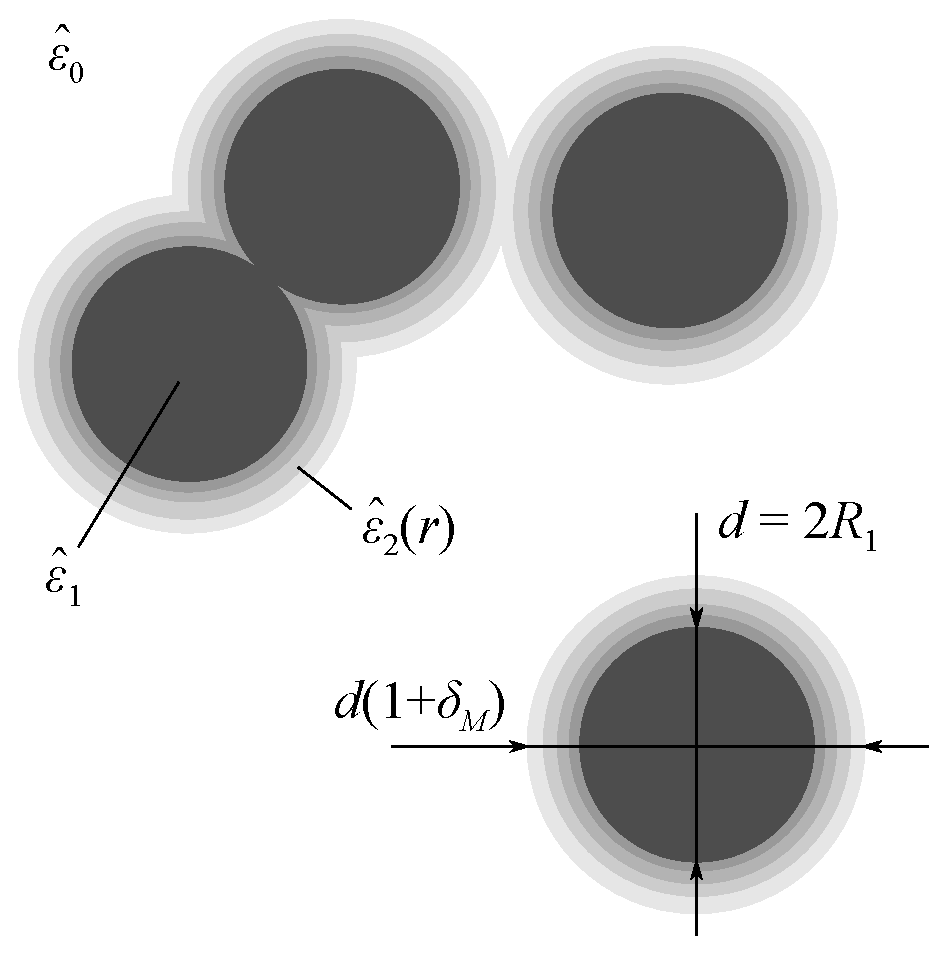
\includegraphics[width=0.5\textwidth]{Fig1_Microstructure_new5.eps}
	\caption{\label{fig:model-Mlayers}
		Модель тривимірної макроскопічно однорідної та ізотропної системи частинок з морфологією тверде ядро - проникна оболонка. Всі частинки знаходяться в однорідній матриці з комплексною проникністю $\hat{\varepsilon}_0$ (біла область) та складаються з твердого ядра радіусом $R_1=d/2$ та комплексною проникністю $\hat{\varepsilon}_1$ (чорні області) та концентричної проникної оболонки товщиною $h=R_1\delta_M$ (сірі області). Оболонки в загальному випадку є електрично неоднорідними з радіальним розподілом комплексної проникності $\hat{\varepsilon}_2(r)$. Локальне значення проникності в точках перекриття компонентів системи визначається відстанню до центра найближчої частинки}
\end{figure} 
Локальне значення проникності $\hat{\varepsilon} ({\bf r})$ в такій моделі можна подати у вигляді ступінчатої функції, що залежить від відстані $l = \min\limits_{1 \leq a \leq N} |{\bf r} - {\bf r}_a|$ від даної точки ${\bf r}$ до центра найближчої частинки. Для електрично однорідних оболонок $\hat{\varepsilon} ({\bf r})$ набирає вигляд:
\begin{equation}\label{eq:local-perm-1layer}
\hat{\varepsilon} ({\bf r}) = \left\{ 
\begin{array}{ll}
\hat{\varepsilon}_0, & l > R_2\\
\hat{\varepsilon}_1, & l < R_1\\
\hat{\varepsilon}_2, & R_1 < l < R_2,
\end{array}
\right.
\end{equation}
де $\hat{\varepsilon}_0$, $\hat{\varepsilon}_1$, $\hat{\varepsilon}_2$ -- комплексні діелектричні проникності, відповідно, матриці (біла область на рис. \ref{fig:model-Mlayers}), ядер (чорні області) та оболонок (сірі області); $R_1$ -- радіус ядра; $R_2$ -- радіус ядра разом зі своєю оболонкою. 

Для узагальнення такого запису $\hat{\varepsilon} ({\bf r})$ на випадок радіально-неоднорідних оболонок з розглядуваним правилом перекриття компонентів спочатку розглядається випадок оболонок, що складаються з  $M$ концентричних шарів, при перекритті яких домінуючими є ближчі до ядра шари (сірі області на рис.~\ref{fig:model-Mlayers}).
Кожен $m$-ий шар ($1 \leq m \leq M$) має зовнішній радіус $R_{2,m} = R_1(1 + \delta_m)$ ($R_{2,m-1}<R_{2,m}$) по відношенню до центра ядра частинки  та проникність $\hat{\varepsilon}_{2,m}$. Локальне значення проникності $\hat{\varepsilon} ({\bf r})$ в такій системі можна записати у наступному вигляді:
\begin{equation}\label{eq:local-perm-Mlayer}
\hat{\varepsilon} ({\bf r}) = \left\{ 
\begin{array}{ll}
\hat{\varepsilon}_0, & l > R_{2,M}\\
\hat{\varepsilon}_1, & l < R_1\\
\hat{\varepsilon}_{2,1}, & R_1 < l < R_{2,1}\\
\hat{\varepsilon}_{2,m}, & R_{2,m-1} < l < R_{2,m},\,\, 2 \leq m \leq M.
\end{array}
\right.
\end{equation}
Отримавши загальні співвідношення для ефективних характеристик такої системи, вони узагальнюються для випадку радіально-неоднорідного кусково-гладкого розподілу $\hat{\varepsilon}_2(r)$ переходом до границь $M \to \infty$, $|\delta_{m} - \delta_{m-1}| \to 0$ при $\delta_M = {\rm const}$ (див. розділ \ref{sec:model-inhomog}).

%Частота тестуючого поля $\omega$ вважається достатньо малою, щоб можна було знехтувати діелектричними втратами. У цьому випадку структура комплексної діелектричної проникності має вигляд~\cite{LandauT8}:
%\begin{equation}\label{eq:eps_complex}
%\hat{\varepsilon} = \varepsilon + i\,\frac{4\pi}{\omega}\sigma
%\end{equation}
%та пов'язана з комплексною провідністю $\hat{\sigma}$ наступним чином~\cite{broadband}:
%\begin{equation}\label{eq:sigma_complex}
%\hat{\sigma} = -i\,\frac{\omega}{4\pi}\,\hat{\varepsilon}
%= \sigma - i\,\frac{\omega}{4\pi}\,{\varepsilon},
%\end{equation}
%де $\varepsilon$ та $\sigma$ -- відповідно, дійсна частина комплексної діелектричної проникності та квазістатична провідність. Вважається, що всі розглядувані комплексні проникності мають таку структуру.

Для реалізації цих моделей в рамках МКГ необхідно спочатку узагальнити цей метод на випадок систем з провідними компонентами. Після отримання загального співвідношення та замикання обчислювальної схеми можна переходити до застосування отриманого результату до розподілів (\ref{eq:local-perm-1layer}) та (\ref{eq:local-perm-Mlayer}).


\section{Узагальнення МКГ на системи з провідними компонентами}\label{sec:CGA_theory}

Для початку відтворимо узагальнене на випадок комплексних діелектричних проникностей рівняння  розповсюдження електромагнітної хвилі на випадок систем з провідними компонентами. 
Для цього розглянемо рівняння Максвелла у Фур'є представленні за часом для тривимірної статистично однорідної та ізотропної дисперсно-подібної системи $\cal{D}$, що складається з провідних немагнітних компонентів:
\begin{equation}\label{eq:MEdiv-D}
{\rm div}\,{\bf D}({\bf r}, \omega) = 4 \pi \rho({\bf r}, \omega),
\end{equation}
\begin{equation}\label{eq:MEdiv-H}
{\rm div}\,{\bf H}({\bf r}, \omega) = 0,
\end{equation}
\begin{equation}\label{eq:MErot-D}
{\rm rot}\,{\bf E}({\bf r}, \omega) = i\frac{\omega}{\rm c} {\bf H}({\bf r}, \omega), 
\end{equation}
\begin{equation}\label{eq:MErot-H}
{\rm rot}\,{\bf H}({\bf r}, \omega) = \frac{4\pi}{\rm c}\,{\bf j}({\bf r}, \omega) - i\frac{\omega}{\rm c} {\bf D}({\bf r}, \omega),
\end{equation}
%\begin{equation} {\label{eq:chargeConservation}}
%-i\omega\rho({\bf r}, \omega) + {\rm div}\,{\bf j}({\bf r}, \omega) = 0,
%\end{equation}
де ${\bf E}$, ${\bf D}$, ${\bf H}$ та ${\bf j}$ -- вектори напруженості та індукції електричного поля, вектор індукції магнітного поля та вектор щільності струму в дисперсній системі; $\rho$ -- щільність вільних зарядів; ${\rm c}$ -- швидкість світла в вакуумі. 

Вважаючи частоти тестуючого поля $\omega$ достатньо малими, щоб внесками діелектричних втрат можна було знехтувати (квазістатичне наближення), матеріальні рівняння для полів ${\bf D}$ та ${\bf j}$ матимуть вигляд:
\begin{equation}\label{eq:materialEquation-D}
{\bf D}({\bf r}, \omega) = \varepsilon({\bf r})\,{\bf E}({\bf r}, \omega);
\end{equation}
\begin{equation}\label{eq:materialEquation-j}
{\bf j}({\bf r}, \omega) = \sigma({\bf r})\,{\bf E}({\bf r}, \omega),
\end{equation}
де $\varepsilon({\bf r})$, $\sigma({\bf r})$ -- локальні значення квазістатичних проникності та провідності, відповідно. 
Після підстановки цих рівнянь до четвертого рівняння Максвелла (\ref{eq:MErot-H}), отримуємо співвідношення:
\begin{equation}\label{eq:MErot-H-material}
{\rm rot}\,{\bf H}({\bf r}, \omega) = \frac{4\pi}{\rm c}\,\sigma({\bf r})\,{\bf E}({\bf r}, \omega) - i\frac{\omega}{\rm c} \varepsilon({\bf r})\, {\bf E}({\bf r}, \omega) = \frac{4\pi}{\rm c}\,{\bf J}({\bf r}, \omega),
\end{equation}
де було введено наступне визначення комплексного струму ${\bf J}$:
\begin{equation}\label{eq:ComplexCurrent-J}
{\bf J}({\bf r}, \omega) = \left(\sigma({\bf r}) - i\frac{\omega}{4\pi} \varepsilon({\bf r}) \right) {\bf E}({\bf r}, \omega) = \hat{\sigma}({\bf r}, \omega)\,{\bf E}({\bf r}, \omega).
\end{equation}
Тут $\hat{\sigma}({\bf r}, \omega)$ --  квазістатична комплексна провідність системи $\cal D$, яка пов'язана із квазістатичною комплексною діелектричною приникністю~\cite{LandauT8}
\begin{equation}\label{eq:eps_complex}
\hat{\varepsilon}({\bf r}, \omega) = \varepsilon ({\bf r}) + i\,\frac{4\pi}{\omega}\sigma({\bf r})
\end{equation}
співвідношенням $\hat{\sigma} = -i\omega {\hat\varepsilon}/4\pi$ \cite{broadband}.
Таке визначення комплексного струму задовольняє закону Ома у статичному наближенні ($\omega\to 0$):
$$
\lim\limits_{\omega \to 0} {\bf J}({\bf r},\omega) = {\bf j}({\bf r}, 0) = \sigma({\bf r}) {\bf E}({\bf r}, 0)
$$
та підкоряється наступному рівнянню, яке можна отримати із рівняння неперервності:
\begin{equation}\label{eq:ComplexCurrent-div}
{\rm div}\,{\bf J}({\bf r}, \omega) = 0.
\end{equation} 
Надалі $\omega$ не буде вказуватись в списку аргументів відповідних величин.

Таке визначення $\bf J$ є коректним та дозволяє працювати з комплексною проникністю $\hat{\varepsilon}$, що має структуру (\ref{eq:eps_complex}), уникаючи точок неаналітичності у статичному наближенні ($\omega \to 0$). Вважається, що всі розглядувані комплексні проникності мають структуру (\ref{eq:eps_complex}).

Підставляючи поле ${\bf H}$ з третього рівняння Максвелла (\ref{eq:MErot-D}) у четверте (\ref{eq:MErot-H}) та записуючи локальне значення комплексної проникності $\hat{\varepsilon}({\bf r})$ в системі $\cal S$, яка відповідає системі $\cal D$, у вигляді суми комплексної проникності $\hat{\varepsilon}_{\rm f}$ допоміжної матриці $\cal M$ та внеску компактної групи $\delta\hat{\varepsilon}({\bf r})$ в даній точці:
$$
\hat{\varepsilon}({\bf r}) = \hat{\varepsilon}_{\rm f} + \delta\hat{\varepsilon}({\bf r}),
$$
отримуємо наступне рівняння розповсюдження електромагнітної хвилі в $\cal S$:
\begin{equation} \label{eq:propogate_eq}
\Delta {\bf E} ({\bf r}) - {\rm grad}\, {\rm div} {\bf E} ({\bf r}) + k_0^{2}\hat{\varepsilon}_{\rm f} {\bf E} ({\bf r})  = - k_{0}^{2} \delta
\hat{\varepsilon} ({\bf r}) {\bf E} ({\bf r})
\end{equation}
та еквівалентне інтегральне рівняння:
\begin{equation}\label{eq:integral_field}
{\bf E}({\rm {\bf r}}) = {\bf E}_{0} ({\bf r}) -
k_{0}^{2} \int\limits_{V} d{\bf r}'\, {\rm T}(|{\bf r} - {\bf r}'|)
\delta \hat{\varepsilon} ({\bf r}')\, {\bf E}({\bf r}').
\end{equation}
Тут $\Delta$ -- оператор Лапласа; $k_0 = \omega/{\rm c}$ -- модуль хвильового вектора падаючої хвилі з циклічною частотою $\omega$ в вакуумі; ${\bf E}_0 ({\bf r}) = {\bf E}_0 e^{i {\bf k}{\bf r}}$;
${\bf E}_0$, ${\bf k} = \sqrt{\hat{\varepsilon}_{\rm f}}\,
{\bf k}_0$ -- відповідно, амплітуда та хвильовий вектор
падаючої хвилі в середовищі з проникністю ${\varepsilon}_{\rm f}$; 
${\rm T}({\bf r}, {\bf r}') = {\rm T}(|{\bf r} - {\bf r}'|)$ -- тензор Гріна (пропагатор) рівняння (\ref{eq:propogate_eq}). Для макроскопічно однорідного та ізотропного середовища декартові компоненти цього тензора 
\begin{equation}\label{eq:propogator-eps-origin}
	T_{\alpha\beta}({\rm {\bf r}}) = -(k^2\delta_{\alpha\beta} + \nabla_\alpha \nabla_\beta)\frac{e^{ikr}}{4\pi k^2r},\qquad k=|{\bf k}|
\end{equation}
можуть бути записані у вигляді~\cite{Ryzhov1965, Weighofer1989, Weiglhofer1995, Sushko2004}:
\begin{eqnarray}\label{eq:propagator-eps}
{\widetilde T}_{\alpha\beta} ({\rm {\bf r}})
= {\widetilde T}_{\alpha\beta}^{(1)} ({\rm {\bf r}}) + {\widetilde T}_{\alpha\beta}^{(2)} ({\rm {\bf r}}) + {\widetilde T}_{\alpha\beta}^{(3)} ({\rm {\bf r}}),
\end{eqnarray}
\begin{equation}\label{eq:propagator-eps-T1}
{\widetilde T}_{\alpha\beta}^{(1)} ({\rm {\bf r}}) = \frac{e^{ikr}}{3k^{2}} \delta({\bf r})\delta_{\alpha\beta};
\end{equation}
\begin{equation}\label{eq:propagator-eps-T2}
{\widetilde T}_{\alpha\beta}^{(2)} ({\rm {\bf r}}) = \frac{1}{4\pi k^{2}}
\left(\frac{1}{r^3}-\frac{ik}{r^2}\right)
\left( \delta _{\alpha\beta} - 3e_{\alpha} e_{\beta}
\right)\,e^{ikr};
\end{equation}
\begin{equation}\label{eq:propagator-eps-T3}
{\widetilde T}_{\alpha\beta}^{(3)} ({\rm {\bf r}}) = - \frac{1}{4\pi r}\left( {\delta
	_{\alpha\beta} - e_{\alpha} e_{\beta}} \right)\,e^{ikr}
\end{equation}
у тому сенсі, що виконується співвідношення
$$
\int\limits_V d{\bf r} \psi({\bf r}) {\rm T}({\bf r}) =
\int\limits_V d{\bf r} \psi({\bf r}) \widetilde{\rm T}({\bf r}).
$$
Представлення (\ref{eq:propagator-eps}) можна отримати з цього співвідношення, розглядаючи виколоту сферичну область радіусу $a\to 0$ з центром у початку координат. Тут $\psi$ -- фінітна обмежена кусково-гладка скалярна функція; $e_\alpha = r_\alpha/r$ -- нормовані компоненти радіус-вектору ${\bf r}$; $\delta_{\alpha\beta}$ -- символ Кронекера; $\delta({\bf r})$ -- дельта-функція Дірака.
Внески ${\widetilde T}_{\alpha\beta}^{(1)}$ та ${\widetilde T}_{\alpha\beta}^{(2)}$ в пропагатор (\ref{eq:propagator-eps})  описують ближні перевипромінювання всередині компактної групи; другий внесок ${\widetilde T}_{\alpha\beta}^{(3)}$ в головну частину описує дальні перевипромінювання між компактними групами \cite{Sushko2007, Sushko2017}.

Ефективну комплексну діелектричну проникність $\hat{\varepsilon}_{\rm eff}$ системи $\cal S$ визначимо через ефективну комплексну провідність $\hat{\sigma}_{\rm eff}$
%Працювати з комплексною провідністю зручніше ніж з проникністю, через відсутність у першій точок неаналітичності у статичному наближенні ($\omega \to 0$). Тому задачу знаходження ефективної комплексної проникності $\hat{\varepsilon}_{\rm eff}$ системи ${\cal D}$ будемо формулювати в термінах комплексної провідності $\hat{\sigma}_{\rm eff}$ у сенсі співвідношення (\ref{eq:sigma_complex}), 
як коефіцієнт пропорційності між статистичними середніми від густини комплексного струму $\langle{\bf J}\rangle$ та напруженості електричного поля $\langle {\bf E} \rangle$:
\begin{equation}\label{eq:eff_complex}
\langle {\bf{J}} ({\bf{r}})\rangle =-i\frac{\omega}{4\pi} \hat{\varepsilon}_{\rm f} \langle {\bf{E}} ({\bf{r}}) \rangle
-i\frac{\omega}{4\pi}\langle \delta\hat{\varepsilon} ({\bf{r}}) {\bf{E}}
({\bf{r}}) \rangle = -i\frac{\omega}{4\pi} \hat{\varepsilon}_{\rm
	eff} \langle {\bf{E}} ({\bf{r}}) \rangle.
\end{equation}
%де локальне значення комплексної проникності $\hat{\varepsilon} ({\bf{r}})$, представлено в термінах МКГ у вигляді суми комплексної проникності $\hat{\varepsilon}_{\rm f}$ допоміжної матриці $\cal M$ та внеску компактної групи $\delta\hat{\varepsilon}({\bf r})$ в даній точці:
%\begin{equation}\label{eq:eps-local}
%\hat{\varepsilon} ({\bf r}) = \hat{\varepsilon}_{\rm f} + \delta\hat{\varepsilon} ({\bf r}).
%\end{equation}
Повторюючи далі такі ж самі розрахунки, що були зроблені в \cite{Sushko2007, Sushko2017}, знаходження $\langle {\bf E}({\bf r}) \rangle$ та $\langle {\bf J}({\bf r}) \rangle$ зводиться до усереднення ітераційного ряду, що містить лише сингулярні внески $\widetilde{T}^{(1)}_{\alpha\beta}$ пропагатора, після розрахунку яких отримуємо:
\begin{equation}\label{eq:E_average-complex}
\langle {\bf E} ({\bf r}) \rangle = \left[ 1 + \langle \hat{Q}({\bf r}) \rangle \right] {\bf E}_0;
\end{equation}
\begin{equation}\label{eq:C_average}
\langle {\bf J} ({\bf r}) \rangle = - i \frac{\omega\hat{\varepsilon}_{\rm f}}{4\pi} \left[ 1 - 2\langle \hat{Q}({\bf r}) \rangle \right] {\bf E}_0,
\end{equation}
де
\begin{equation}\label{eq:Q-complex}
\hat{Q}({\bf r}) = \sum\limits_{s=1}^{\infty} \left( - \frac{1}{3\hat{\varepsilon}_{\rm f}} \right)^s (\delta\hat{\varepsilon}({\bf r}))^s.
\end{equation}
%Можна показати, що цей ряд є асимптотичним наступним чином. 
%
%Якщо перейти до квазістатичного наближення одразу після введення $\widetilde{\rm T}$, залишаючи лише перші порядки за $\omega$ у виразі для $\bf E$, компоненти пропагатора (\ref{eq:propagator-eps}) можна переписати:
%\begin{equation}\label{eq:prop_longwave}
%\lim\limits_{\omega \to 0} k^2 \widetilde{T}_{\alpha\beta} = \tau_{\alpha\beta}^{(1)} + \tau_{\alpha\beta}^{(2)} =
%\frac{1}{3} \delta({\bf r}) \delta_{\alpha\beta} + \frac{\delta_{\alpha\beta} - 3e_\alpha e_\beta}{4\pi r^3}.
%\end{equation}
%Підставляючи цей вираз до (\ref{eq:integral_field}), одразу виділяючи сингулярну частину та після простих алгебраїчних маніпуляцій усереднюючи, отримаємо наступні вирази для середніх полів:
%\begin{equation}\label{eq:E-averaged-direct}
%\langle {\bf E}({\bf r}) \rangle = 
%\left\langle \frac{3\hat{\varepsilon}_{\rm f}}{3\hat{\varepsilon}_{\rm f} + \delta\hat{\varepsilon}({\bf r})} \right\rangle {\bf E}_0 
%- 3 \int\limits_V d{\bf r}' \tau^{(2)} (|{\bf r} - {\bf r}'|) \left\langle \frac{\delta\hat{\varepsilon}({\bf r}')}{3\hat{\varepsilon}_{\rm f} + \delta\hat{\varepsilon}({\bf r})} {\bf E}({\bf r}') \right\rangle ,
%\end{equation}
%\begin{equation}\label{eq:C-averaged-direct}
%\begin{split}
%\langle {\bf J}({\bf r}) \rangle =& 
%- i \frac{\omega}{4\pi} \hat{\varepsilon}_{\rm f} \left[ 1 + 2 \left\langle \frac{\delta\hat{\varepsilon} ({\bf r})}{3\hat{\varepsilon}_{\rm f} + \delta\hat{\varepsilon}({\bf r})} \right\rangle \right] {\bf E}_0 \\
%&+ i \frac{3}{4\pi} \int\limits_V d{\bf r}' \tau^{(2)} (|{\bf r} - {\bf r}'|) \left\langle \frac{\omega \hat{\varepsilon}({\bf r}) \delta\hat{\varepsilon}({\bf r}')}{3\hat{\varepsilon}_{\rm f} + \delta\hat{\varepsilon}({\bf r})} {\bf E}({\bf r}') \right\rangle.
%\end{split}
%\end{equation}
%Для макроскопічно однорідних та ізотропних систем статистичні середні під інтегралами залежать лише від $|{\bf r} - {\bf r}'|$. Тому зважаючи на форму кутової частини $\tau_{\alpha\beta}^{(2)}$, інтеграли в (\ref{eq:E-averaged-direct}) та (\ref{eq:C-averaged-direct}) зануляються.
%Використовуючи (\ref{eq:E-averaged-direct}), (\ref{eq:C-averaged-direct}) разом з (\ref{eq:eff_complex}), отримуємо рівняння (\ref{eq:E_average-complex}) та (\ref{eq:C_average}), де $\hat{Q}$ має вигляд:
%\begin{equation}\label{eq:Q-direct}
%\hat{Q}({\bf r}) = -\frac{\delta\hat{\varepsilon}({\bf r})}{3\varepsilon_{\rm f} + \delta\hat{\varepsilon}({\bf r})}.
%\end{equation}
%Розклавши в ряд Маклорена праву частину цього рівняння за 
%$\delta\hat{\varepsilon}$ отримаємо вираз (\ref{eq:Q-complex}).

Підставляючи вирази для середніх полів (\ref{eq:E_average-complex}), 
(\ref{eq:C_average}) у (\ref{eq:eff_complex}) отримуємо наступне 
рівняння для $\hat{\varepsilon}_{\rm eff}$, що залежить лише від 
$\hat{\varepsilon}_{\rm f}$ та вигляду $\delta\hat{\varepsilon}$:
\begin{equation}\label{eq:general_not_homogenized}
\langle \hat{Q} \rangle = \frac{\hat{\varepsilon}_{\rm f} - \hat{\varepsilon}_{\rm eff}}{2\hat{\varepsilon}_{\rm f} + \hat{\varepsilon}_{\rm eff}}.
\end{equation}


\section{Знаходження $\hat{\varepsilon}_{\rm f}$}\label{sec:eps-f}

Покажемо, що у квазістатичному наближенні сумісною з МКГ є лише умова $\hat{\varepsilon}_{\rm f} = \hat{\varepsilon}_{\rm eff}$.
Для цього спочатку запишемо граничні умови для нормальних компонент електричного поля на межі розділу допоміжної матриці $\cal{M}$ та гомогенізованого середовища $\cal D$~\cite{Sillars1937}:
\begin{equation}\label{eq:boundary}
\hat{\varepsilon}_{\rm f} {\bf E}_{0n} = \hat{\varepsilon}_{\rm eff} \langle {\bf E}({\bf r}) \rangle_{n}.
\end{equation}
Користуючись цією рівністю та виразом (\ref{eq:E_average-complex}), отримуємо 
\begin{equation}\label{eq:system_for_homog}
\langle \hat{Q} \rangle = \frac{\hat{\varepsilon}_{\rm f} - \hat{\varepsilon}_{\rm eff}}{\hat{\varepsilon}_{\rm eff}},
\end{equation}
що разом з (\ref{eq:general_not_homogenized}) дає рівняння для
заходження $\hat{\varepsilon}_{\rm f}$ та $\hat{\varepsilon}_{\rm eff}$:
\begin{equation}
	\frac{\hat{\varepsilon}_{\rm f} - \hat{\varepsilon}_{\rm eff}}{2\hat{\varepsilon}_{\rm f} + \hat{\varepsilon}_{\rm eff}} = \frac{\hat{\varepsilon}_{\rm f} - \hat{\varepsilon}_{\rm eff}}{\hat{\varepsilon}_{\rm eff}}.
\end{equation}
Відкидаючи нефізичний розв'язок 
$\hat{\varepsilon}_{\rm f} = 0$, отримуємо
\begin{equation}\label{eq:homog}
\hat{\varepsilon}_{\rm f} = \hat{\varepsilon}_{\rm eff};
\end{equation}
\begin{equation}\label{eq:general_Q}
\langle \hat{Q} ({\bf r}) \rangle = 0.
\end{equation}
Останнє співвідношення може бути отримано й з варіаційного принципу Ха\-шина-Штрік\-мана, як вже зазначалось в розділі \ref{sec:CGA} для діелектричних систем, розглядаючи окремо проникність та провідність \cite{Sushko2017, Torquato1991}.
%розглядаючи крім чисто діелектричних систем провідні системи, будуючи функціонал $U_{\bf T}$ від ${\bf T} = {\bf j} - \sigma_{\rm f}{\bf E}$, та трактуючи його стаціонарне значення за Джоулеві втрати $U^s_{\bf T} = \langle {\bf E} \rangle \langle {\bf j} \rangle V/8\pi$.

Рівняння (\ref{eq:general_Q}) є строгим у наближенні $\omega \to 0$ для статичної провідності. Для його використання та отримання значення $\hat{\varepsilon}_{\rm eff}$ треба в явному вигляді записати $\delta\hat{\varepsilon}({\bf r})$ для розглядуваної системи та підсумувати ряди в (\ref{eq:Q-complex}).


\section{Ефективна квазістатична діелектрична проникність 
	%модельної 
	системи}

%{\colrr Розглянемо тривимірну макроскопічно однорідну та ізотропну систему частинок з морфологією тверде ядро--проникна оболонка (див. рис.~\ref{fig:model-1layer-b}), де всі проникності комплексні та мають структуру (\ref{eq:eps_complex}). 
%%Локальне значення проникності визначається відстанню від даної точки до центра найближчої частинки.
%Локальне значення проникності $\hat{\varepsilon} ({\bf r})$ такої моделі можна подати у вигляді ступінчатої функції, що залежить від відстані $l = \min\limits_{1 \leq a \leq N} |{\bf r} - {\bf r}_a|$ від даної точки ${\bf r}$ до найближчої частинки та для електрично однорідних оболонок набуває вигляд:
%\begin{equation}\label{eq:local-perm-1layer0}
%\hat{\varepsilon} ({\bf r}) = \left\{ 
%\begin{array}{ll}
%\hat{\varepsilon}_0, & l > R_2\\
%\hat{\varepsilon}_1, & l < R_1\\
%\hat{\varepsilon}_2, & R_1 < l < R_2.
%\end{array}
%\right.
%\end{equation}}
%%%%%%%%%%%%%%%%%%%%%%%%%%%%

\subsection{Випадок електрично однорідних оболонок}

Внесок компактних груп $\delta\hat{\varepsilon}({\bf r})$ для  випадку електрично однорідних оболонок з розподілом  локальної комплексної проникності (\ref{eq:local-perm-1layer}) в системі можна записати у наступному вигляді, використовуючи характеристичні функції $\Pi_1$ та $\Pi_2$ областей, що зайняті, відповідно, всіма ядрами (всі чорні області на рис.~\ref{fig:model-Mlayers}) та всіма ядрами разом з їх оболонками (всі чорні та сірі області):
\begin{equation}\label{eq:delta-eps-1layer}
\delta\hat{\varepsilon} ({\bf r}) = (1 - \Pi_2 ({\bf r})) \Delta\hat{\varepsilon}_0
+ \Pi_1 ({\bf r}) \Delta\hat{\varepsilon}_1
+ (\Pi_2 ({\bf r}) - \Pi_1 ({\bf r})) \Delta\hat{\varepsilon}_2,
\end{equation}
де $\Delta\hat{\varepsilon}_j = [\hat{\varepsilon}_j - 
\hat{\varepsilon}_{\rm f}]$ ($j = 0,1,2$). 
Ці характеристичні функції задовольняють тотожність $$\Pi_1({\bf r})\,\Pi_2({\bf r}) = \Pi_1({\bf r}),$$ використовуючи яку моменти $\delta\hat{\varepsilon}$ можна записати у наступному вигляді:
\begin{equation}\label{eq:moment-1layer}
\langle (\delta\hat{\varepsilon})^p \rangle = (1 - \phi) (\Delta\hat{\varepsilon}_0)^p 
+ c (\Delta\hat{\varepsilon}_1)^p
+ (\phi - c) (\Delta\hat{\varepsilon}_2)^p,
\end{equation}
де $c = \langle \Pi_1({\bf r}) \rangle$ та $\phi = \langle \Pi_2({\bf r}) \rangle$ -- об'ємні концентрації відповідно тільки ядер та ядер разом з їх оболонками. Для $N$ твердих сферичних ядер $\Pi_1$ можна записати, використовуючи функції Хевісайда $\theta$, як це було зроблено у розділі~\ref{sec:CGA}:
\begin{equation}\label{eq:Pi1}
	\Pi_1({\bf r}) = \sum_{n=1}^N \theta(R_1 - |{\bf r} - {\bf r}_n|);
\end{equation}
явний вигляд $\Pi_2$ можна записати у  вигляді~\cite{TorquatoCoreShell, Torquato}
\begin{equation}\label{eq:Pi2}
\Pi_2 ({\bf r}) = 1 - \prod_{n=1}^{N}\left[ 1 - \chi_2^{(n)}({\bf r}) \right] = \sum_{n=1}^{N}\chi_2^{(n)}({\bf r}) - \sum_{n<q}\chi_2^{(n)}({\bf r})\chi_2^{(q)}({\bf r}) + ..., 
\end{equation}
використовуючи одночастинкові характеристичні функції $\chi^{(n)}_2({\bf r})$ областей, зайнятих кожним $n$-им ядром разом з його оболонкою. Для розрахунку об'ємної концентрації 
\begin{equation}\label{eq:phi-full}
\phi = 1 - \left\langle \prod_{n=1}^{N}\left[ 1 - \chi_2^{(n)}({\bf r}) \right] \right\rangle = N \langle \chi_2^{(1)} ({\bf r}) \rangle
- \frac{N(N-1)}{2} \langle \chi_2^{(1)} ({\bf r}) \chi_2^{(2)} ({\bf r}) \rangle + ...
\end{equation}
таких частинок необхідно знати багаточастинкові функції розподілу $F_n({\bf r}; {\bf r}^n)$ (${\bf r}^n = \{{\bf r}_1, {\bf r}_2,..., {\bf r}_n\}$). 

Для розглядуваної моделі сферичних частинок з твердими ядрами та вільно проникними оболонками у статистичній рівновазі можна використовувати  функції розподілу системі твердих сфер з радіусом $R_1$~\cite{Wertheim1963, Lebowitz1964}, які в рамках теорії масштабованих частинок (scaled particle theory~\cite{Reiss1959}) в парному наближенні дають наступний результат для $\phi$~\cite{RikvoldP.1985}: 
\begin{equation}\label{eq:phi_pen}
\begin{split}
\phi(c,\delta) &= 1 - (1-c)\exp{\left[ -\frac{(1-\psi)\phi_t}{1-c} \right]} \times \\
&\times\exp{\left[ -\frac{3c\phi_t}{2(1-c)^3} \left( 2 - 3
	\psi^{1/3} + \psi - c \left( 3\psi^{1/3} - 6\psi^{2/3} +3\psi
	\right) \right) \right]},
\end{split}
\end{equation}
де $\delta = (R_2 - R_1)/R_1$ -- відносна товщина оболонок (див. рис. \ref{fig:model-2layers}); $\psi=(1+\delta)^{-3}$; 
\begin{equation}\label{eq:phi-hard}
\phi_t = c (1+\delta)^3 = c/\psi
\end{equation}
є об'ємною концентрацією ядер з твердими оболонками тієї ж товщини.
Результат (\ref{eq:phi_pen}) добре узгоджується з результатами отриманими в рамках методів Монте-Карло~\cite{Rotter2003} та використовується надалі для розрахунків.

Для знаходження наступного остаточного рівняння для $\hat{\varepsilon}_{\rm eff}$ макроскопічно однорідної та ізотропної тривимірної системи частинок з морфологією тверде ядро~-~проникна електрично однорідна оболонка, підставимо вираз (\ref{eq:moment-1layer}) для моментів $\delta\hat{\varepsilon}$ до (\ref{eq:general_Q}) та підсумуємо отриманий ряд:
%що дає наступний результат для макроскопічно однорідної та ізотропної тривимірної системи частинок з морфологією тверде ядро~-~проникна електрично однорідна оболонка:
\begin{equation}\label{eq:general_1layer_complex}
(1 - \phi(c,\delta)) \frac{\hat{\varepsilon}_0 - \hat{\varepsilon}_{\rm eff}}{2\hat{\varepsilon}_{\rm eff} + \hat{\varepsilon}_0}
+ c \frac{\hat{\varepsilon}_1 - \hat{\varepsilon}_{\rm eff}}{2\hat{\varepsilon}_{\rm eff} + \hat{\varepsilon}_1}
+ (\phi(c,\delta) - c) \frac{\hat{\varepsilon}_2 - \hat{\varepsilon}_{\rm eff}}{2\hat{\varepsilon}_{\rm eff} + \hat{\varepsilon}_2} = 0.
\end{equation}
Через те, що $\hat{\varepsilon}_{\rm eff}$ шукається у квазістатичному наближенні та має форму (\ref{eq:eps_complex}), це рівняння можна спростити користуючись методами теорії збурень. Зокрема, якщо виконуються нерівності
\begin{equation}\label{eq:ineq}
\begin{split}
	|\sigma_j - \sigma_{\rm eff}| \gg \frac{\omega}{4\pi}|\varepsilon_j - \varepsilon_{\rm eff}|,\\
	|\sigma_j + 2\sigma_{\rm eff}| \gg \frac{\omega}{4\pi} |\varepsilon_j + 2\varepsilon_{\rm eff}|,
\end{split}
\end{equation}
для всіх компонентів системи ($j=0,1,2$), рівняння (\ref{eq:general_1layer_complex}) зводиться до системи наступних двох дійсних рівнянь для ефективних квазістатичних провідності $\sigma_{\rm eff}$ та діелектричної проникності $\varepsilon_{\rm eff}$, відповідно:
\begin{subequations}
	\begin{equation}\label{eq:general_1layer_sigma}
	(1 - \phi) \frac{\sigma_0 - \sigma_{\rm eff}}{2\sigma_{\rm eff} + \sigma_0}
	+ c \frac{\sigma_1 - \sigma_{\rm eff}}{2\sigma_{\rm eff} + \sigma_1}
	+ (\phi - c) \frac{\sigma_2 - \sigma_{\rm eff}}{2\sigma_{\rm eff} + \sigma_2} = 0,
	\end{equation}
	\begin{equation}\label{eq:general_1layer_eps}
	(1 - \phi) \frac{\varepsilon_0\sigma_{\rm eff} - \varepsilon_{\rm eff}\sigma_0}{(2\sigma_{\rm eff} + \sigma_{0})^2} 
	+ c \frac{\varepsilon_1\sigma_{\rm eff} - \varepsilon_{\rm eff}\sigma_1}{(2\sigma_{\rm eff} + \sigma_1)^2}
	+ (\phi - c) \frac{\varepsilon_2\sigma_{\rm eff} - \varepsilon_{\rm eff}\sigma_2}{(2\sigma_{\rm eff} + \sigma_2)^2} = 0.
	\end{equation}
\end{subequations}
Рівняння (\ref{eq:general_1layer_sigma}) для електричної провідності $\sigma_{\rm eff}$ стає строгим у статичному наближенні ($\omega \to 0$); у квазістатичному наближенні умови застосовності (\ref{eq:ineq}) для рівняння (\ref{eq:general_1layer_sigma}) можна спростити:
\begin{equation}\label{eq:ineq-one}
|\sigma_j - \sigma_{\rm eff}| \gg \frac{\omega}{4\pi} |\varepsilon_j + 2\varepsilon_{\rm eff}|, \quad j=0,1,2.
\end{equation}
За інших умов, для отримання співвідношень для квазістатичних $\sigma_{\rm eff}$ та $\varepsilon_{\rm eff}$ потрібен додатковий аналіз рівняння (\ref{eq:general_1layer_complex}).


\subsection{Випадок електрично неоднорідних оболонок}\label{sec:model-inhomog}

Для отримання співвідношення для $\hat{\varepsilon}_{\rm eff}$ у випадку електрично неоднорідних оболонок з радіальним розподілом комплексної проникності спочатку запишемо внески компактних груп $\delta\hat{\varepsilon}$ для випадку розподілу (\ref{eq:local-perm-Mlayer}) для оболонок, що складаються з $M$ електрично однорідних  шарів, використовуючи характеристичні функції $\Pi_1$ та $\Pi_{2,m}$ областей, зайнятих ядрами та ядрами разом з $m$ найближчими до них шарами, відповідно:
\begin{equation}\label{eq:delta-eps-Mlayers}
\begin{split}
\delta\hat{\varepsilon} ({\bf r}) =& (1 - \Pi_{2,M} ({\bf r})) \Delta\hat{\varepsilon}_0
+ \Pi_1 ({\bf r}) \Delta\hat{\varepsilon}_1
+ (\Pi_{2,1} ({\bf r}) - \Pi_{1} ({\bf r})) \Delta\hat{\varepsilon}_{2,1} +\\
&+ \sum\limits_{m=2}^M (\Pi_{2,m} ({\bf r}) - \Pi_{2,m-1} ({\bf r})) \Delta\hat{\varepsilon}_{2,m},
\end{split}
\end{equation}
де $\Delta\hat{\varepsilon}_{2,m} = [\hat{\varepsilon}_{2,m} - \hat{\varepsilon}_{\rm f}]$ ($m=1..M$) -- різниця між комплексною діелектричною проникністю $m$-го шару та проникністю допоміжної матриці $\cal M$. Характеристичні функції $\Pi_{2,m}$ мають ту саму форму, що й для однорідних оболонок (див. (\ref{eq:Pi2})):
\begin{equation}\label{eq:Pi2m}
\Pi_{2,m} ({\bf r}) = 1 - \prod\limits_{n=1}^N \left( 1 - \chi_{2,m}^{(n)} ({\bf r}) \right)
\end{equation}
та задовольняють наступним тотожностям:
\begin{equation}\label{eq:Pi2m-ortho}
	\Pi_1 \Pi_{2,m}  = \Pi_1,\qquad
	\Pi_{2,q} \Pi_{2,m} = \Pi_{2,q} \quad(q<m).
\end{equation}
Тут $\chi_{2,m}^{(n)} ({\bf r}) = \theta(R_{2,m} - |{\bf r} - {\bf r}_n|)$ -- одночастинкова характеристична функція $n$-ої сферичної частинки разом з її $m$ найближчими до ядра шарами.
Використовуючи тотожності (\ref{eq:Pi2m-ortho}), моменти $\delta\hat{\varepsilon}$ можна записати у наступному вигляді:
\begin{equation}\label{eq:moment-Mlayer}
\begin{split}
\langle (\delta\hat{\varepsilon})^p \rangle =& 
(1 - \phi(c,\delta_M)) (\Delta\hat{\varepsilon}_0)^p + 
c (\Delta\hat{\varepsilon}_1)^p + (\phi(c,\delta_1) - c) (\Delta\hat{\varepsilon}_{2,1})^p + \\
&+\sum\limits_{m=2}^M (\phi(c,\delta_m) - \phi(c,\delta_{m-1})) (\Delta\hat{\varepsilon}_{2,m})^p,
\end{split}
\end{equation}
де $\phi(c,\delta_m) = \langle \Pi_{2,m} ({\bf r}) \rangle$ -- об'ємна концентрація областей всіх ядер разом з їх $m$ найближчими шарами, яка для сферичних частинок дається виразом (\ref{eq:phi_pen}). 
Підставляючи моменти (\ref{eq:moment-Mlayer}) до (\ref{eq:general_Q}), отримуємо наступне остаточне співвідношення для $\hat{\varepsilon}_{\rm eff}$ макроскопічно однорідної та ізотропної системи твердих ядер, покритих  $M$ концентричними проникними шарами, при перекритті яких домінуючими є найближчі до ядра шари:
\begin{equation}\label{eq:general_Mlayer_complex}
\begin{split}
(1 - \phi(c,\delta_M)) \frac{\hat{\varepsilon}_0 - \hat{\varepsilon}_{\rm eff}}{2\hat{\varepsilon}_{\rm eff} + \hat{\varepsilon}_0}
+ c \frac{\hat{\varepsilon}_1 - \hat{\varepsilon}_{\rm eff}}{2\hat{\varepsilon}_{\rm eff} + \hat{\varepsilon}_1} + (\phi(c,\delta_1)-c) \frac{\hat{\varepsilon}_{2,1} - \hat{\varepsilon}_{\rm eff}}{2\hat{\varepsilon}_{\rm eff} + \hat{\varepsilon}_{2,1}} +& \\
+ \sum\limits_{m=2}^{M} (\phi(c,\delta_m)-\phi(c,\delta_{m-1})) \frac{\hat{\varepsilon}_{2,m} - \hat{\varepsilon}_{\rm eff}}{2\hat{\varepsilon}_{\rm eff} + \hat{\varepsilon}_{2,m}} &= 0.
\end{split}
\end{equation}

Переходячи до границь $M \to \infty$, $|\delta_{m} - \delta_{m-1}| \to 0$ при $\delta_M = {\rm const}$ та вимагаючи, щоб $\phi (c, u)$ була диференційована за $u$ та прямувала $c$ при $u\to 0$, отримуємо наступне інтегральне рівняння для $\hat{\varepsilon}_{\rm eff}$ системи частинок з морфологією тверде ядро~-~проникна оболонка, де оболонки мають кусково-гладкий радіальний профіль комплексної проникності $\hat{\varepsilon}_{2} (r)$, а локальне значення проникності при їх перекритті визначається профілем найближчої до даної точки частинки:
\begin{equation}\label{eq:general_Contlayer_complex}
(1 - \phi(c,\delta_M)) \frac{\hat{\varepsilon}_0 - \hat{\varepsilon}_{\rm eff}}{2\hat{\varepsilon}_{\rm eff} + \hat{\varepsilon}_0}
+ c \frac{\hat{\varepsilon}_1 - \hat{\varepsilon}_{\rm eff}}{2\hat{\varepsilon}_{\rm eff} + \hat{\varepsilon}_1}
+ \int\limits_0^{\delta_M} \frac{\partial \phi(c,u)}{\partial u} \frac{\hat{\varepsilon}_2 (u) - \hat{\varepsilon}_{\rm eff}}{2\hat{\varepsilon}_{\rm eff} + \hat{\varepsilon}_2 (u)} du = 0.
\end{equation}
де функція $\hat{\varepsilon}_2 (r)$ виражена в термінах змінної $u = (r - R_1)/R_1$.
Таке ж саме співвідношення можна отримати перейшовши до зазначених границь у виразі (\ref{eq:moment-Mlayer}) для моментів $\delta\hat{\varepsilon}$:
\begin{equation}\label{eq:moment-integral}
\langle (\delta\hat{\varepsilon})^p \rangle = 
(1 - \phi(c,\delta)) (\Delta\hat{\varepsilon}_0)^p + 
c (\Delta\hat{\varepsilon}_1)^p + 
\int\limits_{0}^{\delta_M} \frac{\partial \phi(c,u)}{\partial u} (\Delta\hat{\varepsilon}_2 (u))^p \, du,
\end{equation}
та підставляючи цей вираз до (\ref{eq:general_Q}).

Для електрично однорідних оболонок ($\hat{\varepsilon}_2 (u) = {\rm const}$) співвідношення (\ref{eq:general_Contlayer_complex}) зводиться до (\ref{eq:general_1layer_complex}) з $\delta = \delta_M$.

Якщо виконуються нерівності (\ref{eq:ineq}), в рамках теорії збурень рівняння (\ref{eq:moment-integral}) можна звести до системи двох рівнянь для $\sigma_{\rm eff}$ та $\varepsilon_{\rm eff}$, відповідно:
%\begin{subequations}
\begin{equation}\label{eq:general_Contlayer_sigma}
(1 - \phi(c,\delta_M)) \frac{\sigma_0 - \sigma_{\rm eff}}{2\sigma_{\rm eff} + \sigma_0}
+ c \frac{\sigma_1 - \sigma_{\rm eff}}{2\sigma_{\rm eff} + \sigma_1}
+ \int\limits_0^{\delta_M} \frac{\partial \phi(c,u)}{\partial u} \frac{\sigma_2 (u) - \sigma_{\rm eff}}{2\sigma_{\rm eff} + \sigma_2 (u)} du = 0,
\end{equation}
\begin{equation}\label{eq:general_Contlayer_eps}
(1 - \phi) \frac{\varepsilon_0\sigma_{\rm eff} - \varepsilon_{\rm eff}\sigma_0}{(2\sigma_{\rm eff} + \sigma_{0})^2} 
+ c \frac{\varepsilon_1\sigma_{\rm eff} - \varepsilon_{\rm eff}\sigma_1}{(2\sigma_{\rm eff} + \sigma_1)^2}
+ \int\limits_0^{\delta_M} \frac{\partial \phi(c,u)}{\partial u} \frac{\varepsilon_2 (u)\sigma_{\rm eff} - \varepsilon_{\rm eff}\sigma_2 (u)}{(2\sigma_{\rm eff} + \sigma_2 (u))^2} du = 0.
\end{equation}
%\end{subequations}

Зазначимо, що якщо ми не будемо використовувати граничні
умови (\ref{eq:boundary}) для знаходження комплексної проникності $\hat{\varepsilon}_{\rm f}$, з'являється свобода у виборі значення останньої. Її різні значення будуть давати
різні співвідношення для $\hat{\varepsilon}_{\rm eff}$ згідно
(\ref{eq:general_not_homogenized}); так, наприклад, поклавши
$\hat{\varepsilon}_{\rm f} = \hat{\varepsilon}_0$
отримуємо співвідношення типу Максвелла-Гарнетта 
(див.~\cite{Sushko2007,Sushko2009,Sushko2017} та розділ \ref{sec:CGA}) для модельних систем частинок з морфологією тверде ядро~-~проникна оболонка:
\begin{equation}\label{eq:MG-core-shell}
\frac{\hat{\varepsilon}_{\rm eff} - \hat{\varepsilon}_0}{2\hat{\varepsilon}_0 + \hat{\varepsilon}_{\rm eff}} = 
c \frac{\hat{\varepsilon}_1 - \hat{\varepsilon}_0}{2\hat{\varepsilon}_0 + \hat{\varepsilon}_1}
+ \int\limits_0^{\delta_M} \frac{\partial \phi(c,u)}{\partial u} \frac{\hat{\varepsilon}_2 (u) - \hat{\varepsilon}_0}{2\hat{\varepsilon}_0 + \hat{\varepsilon}_2 (u)} du,
\end{equation}
що у статичному наближенні зводиться до наступного співвідношення для
$\sigma_{\rm eff}$:
\begin{equation}\label{eq:MG-core-shell-sigma}
\frac{\sigma_{\rm eff} - \sigma_0}{2\sigma_0 + \sigma_{\rm eff}} = 
c \frac{\sigma_1 - \sigma_0}{2\sigma_0 + \sigma_1}
+ \int\limits_0^{\delta_M} \frac{\partial \phi(c,u)}{\partial u} \frac{\sigma_2 (u) - \sigma_0}{2\sigma_0 + \sigma_2 (u)} du.
\end{equation}


\section{Висновки}

Побудовано електродинамічну тривимірну модель макроскопічно однорідної та ізотропної системи немагнітних сферичних частинок з морфологією тверде ядро~-~проникна оболонка на базі МКГ. Розглядалися два типи оболонок: електрично однорідні та неоднорідні з радіальним розподілом комплексної діелектричної проникності. Локальне значення комплексної проникності в точках перекриття компонентів визначається відстанню до найближчої частинки. 
Для отримання остаточних співвідношень, спершу МКГ узагальнено на випадок систем з провідними компонентами. Замикання теорії виконано, використовуючи граничні умови для нормальних компонентів комплексного електричного поля на межі розділу допоміжної матриці та гомогенізованого середовища. 
Мікроструктура системи моделювалась, використовуючи характеристичні функції областей кожного з компонентів системи.
В результаті отримано співвідношення для ефективної квазістатичної комплексної проникності розглядуваної модельної системи, як функцію від комплексних проникностей компонентів системи та їх об'ємних концентрацій.
Форма частинок грала роль лише при розрахунку явного вигляду функції $\phi$, використовуючи відповідні функції розподілу; в загальному випадку, результати (\ref{eq:general_1layer_complex}) та (\ref{eq:general_Contlayer_complex}) можуть бути застосовані до будь-яких багатофазних макроскопічно однорідних та ізотропних систем у квазістатичному наближенні з відповідною функцією $\phi$.
Отримані результати є основою для подальшого аналізу.
%Очікується, що запропонована модель спроможна ефективно врахувати основні фізико-хімічні механізми в системі, які грають роль у формуванні її ефективних електрофізичних властивостей.

Результати розділу представлено в публікаціях \cite{Sushko2013,Sushko2018PRE}.

Перед тим як застосовувати отримані результати до реальних систем, необхідно протестувати теорію на даних числових симуляцій, в яких відсутні похибки, пов'язані з неконтрольованими процесами та механізмами, що часто з'являються в процесі створення реальних зразків.

%Загальний розв'язок співвідношення (\ref{eq:general_1layer_complex}) робиться за допомогою формул Кардано, а  (\ref{eq:general_Contlayer_complex}) -- тільки використовуючи спеціальний вигляд $\hat{\varepsilon}_2 (u)$, однак аналіз основних характеристик моделі більш практично робити для окремих класів систем.



%%%%%%%%%%%%%%%%%%%%%%%%%%%%%%%%%%%%%%%%%%%%%%%
\chapter{Тестування моделі та її застосування до аналізу провідності композитних електролітів}\label{sec:RRN-electrol}
%%%%%%%%%%%%%%%%%%%%%%%%%%%%%%%%%%%%%%%%%%%%%%%

В даному розділі увага зосереджується на тестуванні та практичних застосуваннях результатів (\ref{eq:general_1layer_sigma}) та (\ref{eq:general_Contlayer_sigma}) для квазістатичної електричної провідності $\sigma_{\rm eff}$ у випадку $\sigma_{0}, \sigma_1 \ll \sigma_2$, який є характерним для твердих композитних (ТКЕ) та полімерних композитних (ПКЕ) електролітів.

Тестування моделі виконується шляхом порівняння її результатів з широким масивом даних числових симуляцій~\cite{Siekierski2005, Siekierski2006, Siekierski2007} для залежностей об'ємної концентрації оболонок та статичної провідності розглядуваної модельної системи від концентрації ядер для різних діаметрів ядер та товщин оболонок двох типів: електрично однорідних~\cite{Siekierski2005, Siekierski2007} та електрично неоднорiдних з гаусовим радіальним профілем провідності~\cite{Siekierski2006}.

Далі модель використовується для обробки та аналізу експериментальних даних для залежностей $\sigma_{\rm eff}$ від об'ємної концентрації дисперсної фази для різних типів композитних електролітів. Зокрема, наводяться результати її застосування до даних \cite{Liang1973} з квазістатичної електричної провідності ТКЕ, утвореного диспергуванням частинок $\rm Al_2O_3$ в полікристалічну матрицю $\rm LiI$, та аналізується питання фізичної інтерпретації цих результатів;
наводяться результати застосування аналогічної процедури до опису експериментальних даних~\cite{Przl1995, Wiec1994} з концентраційних залежностей електричної провідності ПКЕ на основі поліетилен-оксиду (PEO) та PEO з приєднаним оксіметиленом (OMPEO) з додаванням солей $\rm NaI$ або $\rm LiClO_4$. В якості наповнювачів виступали або провідні частинки NASICON ($\rm Na_{3.2} Zr_2P_{0.8} Si_{2.2} O_{12}$), або непровідні частинки $\rm \theta -Al_2O_3$, або поліакриламід (PAAM), що не змішувався з полімером матриці. Наприкінці розділу показується як можна розширити можливості моделі на прикладі вивчення температурної залежності ефективної провідності ПКЕ $\rm OMPEO-LiClO_4-PAAM$.



\section{Тестування моделі за даними симуляцій RRN}\label{sec:RRN-test}

Алгоритм симуляцій Random Resistor Network (RRN)~\cite{Siekierski2005, 
	Siekierski2006, Siekierski2007} 
складається з наступних трьох кроків (див. рис.~\ref{fig:RRN}).

\begin{figure}[!hb]
	\centering
	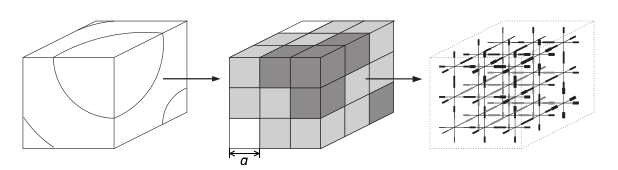
\includegraphics[width=0.95\textwidth]{RRN.png}\\
	(а) \qquad\qquad\qquad\qquad\qquad (б) \qquad\qquad\qquad\qquad\qquad (в)
	\caption{\label{fig:RRN} Етапи алгоритму RRN: (а) модельна система частинок з морфологією тверде ядро~-~проникна оболонка; (б) її апроксимація системою кубів; (в) отримана тривимірна кубічна ґратка резисторів. Рисунок взято з~\cite{Siekierski2007}}
\end{figure}

\begin{enumerate}[label=\alph*)]
	\item Генерація досліджуваної тривимірної системи частинок з 
	морфологією тверде ядро~-~проникна оболонка. Розглядається 
	тривимірний замкнутий простір із заданими розмірами та 
	періодичними граничними умовами. Центри ядер кожної
	частинки розташовуються по черзі наступним чином:
	координати центру поточного ядра генеруються за рівноважним 
	розподілом; якщо отримані координати передбачають перекриття поточного ядра з 
	будь-яким вже згенерованим ядром, вони відкидаються та генеруються 
	нові. Цей процес повторюється доки не буде отримана 
	бажана об'ємна концентрація ядер $c$. Вважається, що
	навколо кожного ядра існує концентрична проникна оболонка з деякою 
	товщиною та радіальним розподілом провідності.
	
	\item Генерація системи кубічних комірок на базі попередньо 
	згенерованої моделі. Для цього розглядається тривимірний
	простір з тими ж розмірами, що й в попередньому випадку, 
	розбитий на кубічні комірки із заданою довжиною ребра $a$. 
	Цей простір накладається на попередньо згенеровану модель. 
	Якщо центр комірки попадає в область ядра, вважається, що 
	ця комірка має такі ж електричні властивості що й 
	ядро. Аналогічно для оболонки та матриці. При цьому алгоритм 
	побудовано так, що виконується умова рівності об'ємної 
	концентрації $c'$ комірок, що відповідають ядрам, та об'ємної концентрації самих ядер $c$.
	
	\item Побудова кубічної ґратки резисторів з отриманої системи
	комірок. Вважається, що центри комірок є вузлами 
	шуканої ґратки. Значення імпедансу кожного резистора (ребра ґратки) розраховується, як для плоского конденсатора, утвореного послідовним з'єдненням половин відповідних двох сусідніх комірок.
	Вважається, що ефективні електричні властивості отриманої 
	ґратки еквівалентні властивостям початкової моделі сферичних частинок.
\end{enumerate}

Для адекватного тестування розвинутої теорії на результатах 
таких симуляцій треба врахувати особливості алгоритму. 


\subsection{Аналіз алгоритму симуляцій}
\subsubsection{Зміна геометричних параметрів оболонок}

В рамках зазначеного алгоритму при заданому абсолютному значенні товщини оболонок $h$, їх відносна товщина $\delta$ після переходу від моделі (а) до моделі (б) змінюється. Дійсно, розглянемо систему (б) об'ємом $V$, яка отримана із системи (а) так, що на кожне ядро в (а) діаметром $d'$ припадає одна комірка в (б) з довжиною ребра $d'$. У такому випадку для $N$ частинок об'ємна концентрація ядер, яка отримується з симуляцій, дорівнює $c' = d'^3 N/V$, а відносна товщина оболонок -- $\delta' = 2h/d'$. 
Для того, щоб виконувалась вимога алгоритму $c' = c$, необхідно, щоб діаметр ядер в (а) дорівнював $d = (\pi/6)^{-1/3} d'$. 
%в якому знаходяться $N$ частинок, ядра яких мають радіус $R_1 = d/2$, а оболонки -- товщину $h = R_1\delta$; тоді $c = (\pi/6) d^3 N/V$ та $\delta = 2h/d$. Нехай на одне ядро припадає одна комірка з довжиною ребра $d'$; об'ємна концентрація таких комірок дорівнює $c' = d'^3 N/V$. Тоді вимога алгоритму $c = c'$ виконується, якщо $d' = (\pi/6)^{1/3} d$. 
Відповідно, відносна товщина $\delta = 2h/d$ буде дорівнювати
%$\delta' = 2h/d'$ після переходу до системи (б) буде дорівнювати
\begin{equation}\label{eq:K-delta-def}
\delta = K \delta',
\end{equation}
де наразі $K = k \equiv (\pi/6)^{1/3} \approx 0.806$. Вважаючи параметр $K$ підгінним, можна узагальнити (\ref{eq:K-delta-def}) на випадок, коли на одну кульку припадає більше ніж одна комірка; чим більша кількість цих комірок, тим ближче значення $K$ до одиниці. Таким чином у загальному випадку виконується нерівність:
\begin{equation}\label{eq:K-delta-ineq}
k \leq K \leq 1 .%\approx 1.241 k.
\end{equation}
В симуляціях~\cite{Siekierski2005, Siekierski2006, Siekierski2007}, довжини ребер комірок $d'$ були $0.5$~мкм, а діаметри ядер варіювалися від 3 до 11~мкм, тож відхилення $K$ від одиниці повинні бути помітними. 

Необхідність використання параметру $K$ підтверджується порівнянням розрахунків залежності об'ємної концентрації оболонок $\phi-c$ від об'ємної концентрації ядер $c$, отриманих в рамках RRN \cite{Siekierski2007} та в рамках перевіреного теоретичного результату (\ref{eq:phi_pen}) (див. рис.~\ref{fig:simulations-phi-a}, \ref{fig:simulations-phi-b}).
\begin{figure}[!ht]
	\centering
		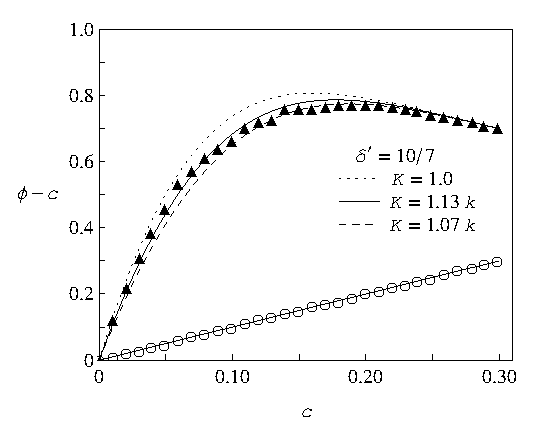
\includegraphics[width=0.48\textwidth]{SiekierskiShell_107.eps}
		\caption{Залежність об'ємної концентрації оболонок $\phi-c$ від об'ємної концентрації ядер $c$ \cite{Siekierski2007} при товщині $h=5$~мкм та $d = 7$ ($\blacktriangle$); пусті точки ($\circ$) -- дані для $c'$. Неперервні лінії -- найкращі результати обробки за формулами (\ref{eq:phi_pen}) та (\ref{eq:K-delta-def}); точкова лінія -- обробка за (\ref{eq:phi_pen}) без використання $K$ ($K=1$ в (\ref{eq:K-delta-def}))} \label{fig:simulations-phi-a}
\end{figure}
{\color{violet} Найбільша середньоквадратична 
похибка представлених найкращих обробок (неперервні лінії) 
дорівнює $0.014$ для даних при $d=7$~мкм, $K=1.13\,k \approx 0.91$.} Без цього параметру розрахунки за (\ref{eq:phi_pen}) дають завищений результат у порівнянні з отриманим в рамках RRN.
Також зазначимо, що знайдені значення $K$ задовольняють наведеній 
вище нерівності (\ref{eq:K-delta-ineq}).

\begin{figure}[t]
	\centering
		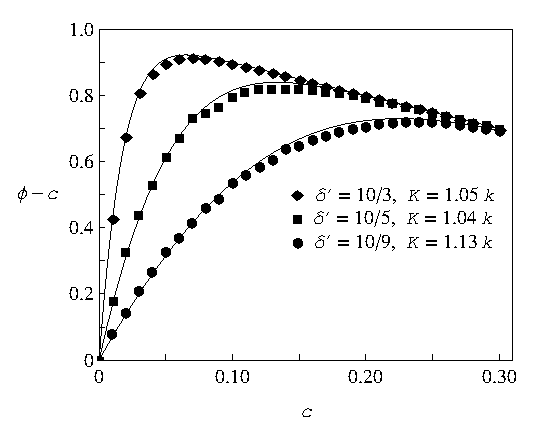
\includegraphics[width=0.48\textwidth]{SiekierskiShell_103-9.eps}
		\caption{Залежності об'ємних концентрацій оболонок $\phi-c$ від об'ємної концентрації ядер $c$ \cite{Siekierski2007} при фіксованій товщині $h=5$~мкм та  $d = 3$ ($\blacklozenge$), 5 ($\blacksquare$), та $9$ ($\bullet$) мкм. Неперервні лінії -- найкращі результати обробки за формулами (\ref{eq:phi_pen}) та (\ref{eq:K-delta-def})} \label{fig:simulations-phi-b}
\end{figure}


\subsubsection{Зміна електричних параметрів неоднорідних оболонок}

У роботі~\cite{Siekierski2006} профіль провідності оболонок $\sigma_2(u)$ моделювався у вигляді гаусового сферично-симетричного розподілу, максимум $\sigma_{\rm max}$ якого знаходився на відстані $h/2$ від поверхні ядра, а мінімум $\sigma_{\rm min}$ -- на зовнішніх границях оболонки. Правило перекриття оболонок те ж саме, що й у розвинутій в розділі \ref{sec:core-shell} моделі.  Явний вигляд профілю $\sigma_2(u)$ та правило, за яким кожній комірці в області оболонки ставилось у відповідність значення провідності, не були зазначені у роботі~\cite{Siekierski2006}, але, базуючись на наявному визначенні $\sigma_2(u)$, у найпростішій формі його можна записати у наступному вигляді:
\begin{equation}\label{eq:GaussianProfile}
\sigma_2(u)=\sigma_{\rm max} \exp
\left[-\frac{4\left(u-\delta/2\right)^2}{{\delta}^2}\ln\left(\frac{\sigma_{\rm
		max}}{\sigma_{\rm min}} \right)\right].
\end{equation}
Нехай $n = h/d'$ є середнє число комірок, що припадають на радіальну 
товщину оболонки; центр першої найближчої до ядра комірки знаходиться у точці $u_1 = \delta'/2n$, другої -- $u_2 = u_1 + \delta'/n = 3u_1$ та, за індукцією, $i$-ої -- $u_i = (2i - 1)u_1 = (2i - 1)\delta'/2n$,
$i = 1..n$. Якщо провідність $i$-ої комірки визначалась як значення функції $\sigma_2(u)$ у точці $u_i$ при відносній товщині $\delta'$ у (\ref{eq:GaussianProfile}), тоді значення параметру $\sigma'_{\rm max}$ в симуляціях \cite{Siekierski2006} визначається точкою $u_{n/2}$ (та $u_{n/2+1}$, якщо $n$ непарне), а значення $\sigma'_{\rm min}$ -- точками $u_1$ та $u_n$:
$$
\sigma'_{\rm max} = \sigma_2(u_{n/2})=\sigma_2(u_{n/2+1})=
\sigma_{\rm max}\left(\frac{ \sigma_{\rm max}}{
	\sigma_{\rm min}}\right)^{-1/n^2},
$$
$$
\sigma'_{\rm min} = \sigma_2(u_{1})=\sigma_2(u_{n})=
\sigma_{\rm max}\left(\frac{ \sigma_{\rm max}}{
	\sigma_{\rm min}}\right)^{-(n-1)^2/n^2}.
$$ 
У наближенні $n \to \infty$: $\sigma'_{\rm max} = \sigma_{\rm max}$ та
$\sigma'_{\rm min} = \sigma_{\rm min}$; для скінченних $n$ виконуються нерівності
$\sigma'_{\rm max} < \sigma_{\rm max}$, $\sigma'_{\rm min}
> \sigma_{\rm min}$, та
\begin{equation}\label{eq:sigma-maxmin-rel}
\frac{\sigma'_{\rm max}}{\sigma'_{\rm min}} = \left(\frac{ \sigma_{\rm max}}{
	\sigma_{\rm min}}\right)^{(n-2)/n}.
\end{equation}
Тобто значення параметрів профілю (\ref{eq:GaussianProfile}) після переходу від системи (а) до системи (б) змінюються та залежать від деталей самого алгоритму. Ці деталі не були зазначені в роботі~\cite{Siekierski2006}, тому для обробки даних, використовуючи профіль (\ref{eq:GaussianProfile}), один з параметрів будемо вважати підгінним, а інший -- фіксованим у значенні, даному в~\cite{Siekierski2006}; наразі $\sigma_{\rm max}$ був вибраний у якості підгінного.


\subsection{Результати тестування}
\subsubsection{Випадок однорідних оболонок}

Спираючись на отриманий результат ми можемо приступити до тестування 
рівняння (\ref{eq:general_1layer_sigma}) для провідності
систем частинок з електрично однорідними оболонками на даних симуляцій 
RRN~\cite{Siekierski2007}. 
На рис. \ref{fig:simulations-sigma-1layer2007-a} та
\begin{table}[!b]
	\begin{center}%\centering
		\caption{\label{tab:RRN-exper-params} Значення провідностей компонентів системи, що використовувались в числових симуляціях RRN~\cite{Siekierski2005, Siekierski2006, Siekierski2007}.}
		\begin{tabular}{|l|c|c|c|c|c|}
			\hline
			Симуляції  & $\sigma_0$, См/см & $\sigma_1$, См/см & $\sigma_2$, См/см & $\sigma_{\rm min}$, См/см & $\sigma_{\rm max}$, См/см \\
			\hline
			\cite{Siekierski2005,Siekierski2007}  & $1\times 10^{-8}$ & $1\times 10^{-12}$ & $1\times 10^{-4}$     & & \\
			\hline
			\cite{Siekierski2006}  & $1\times 10^{-8}$ & $1\times 10^{-12}$ &   & $1\times 10^{-6}$ & $1\times 10^{-4}$\\
			\hline
		\end{tabular}
	\end{center}
\end{table}
\ref{fig:simulations-sigma-1layer2007-b} представлено результати обробки даних симуляцій \cite{Siekierski2007} для концентраційних залежностей ефективної статичної провідності $\sigma_{\rm eff}$. Використані  для симуляцій параметри подано в Таблиці~\ref{tab:RRN-exper-params}. 

\begin{figure}[t]
	\centering
%	\begin{subfigure}[c]{0.48\textwidth}
		\begin{overpic}[width=0.5\textwidth]{SiekierskiShellConductivity_105-9.eps}
			\put(56,17){$\bullet$ -- $d = 9$ мкм}
			\put(56,17){$\bullet$ -- $d = 9$ мкм}
			\put(55,25){$\blacktriangle$ -- $d = 7$ мкм}
			\put(55,33){$\blacksquare$ -- $d = 5$ мкм}
		\end{overpic}
		\caption{Залежності ефективної статичної провідності від концентрації при фіксованій товщині оболонки $h=5$~мкм та різних діаметрах ядер частинок з електрично однорідними оболонками \cite{Siekierski2007} (чорні точки) та їх обробка за (\ref{eq:general_1layer_sigma}), використовуючи значення $\phi$, що були отримані в рамках симуляцій (рис.~\ref{fig:simulations-phi-b}) (пусті точки)} \label{fig:simulations-sigma-1layer2007-a}
%	\end{subfigure}
%	\quad
%	\begin{subfigure}[c]{0.48\textwidth}
%		\begin{overpic}[width=\textwidth]{Fig5_SiekierskiConductivity107a_4.eps}
%			\put(68,68){$d = 7$ мкм}
%		\end{overpic}
%		\caption{} \label{fig:simulations-sigma-1layer2007-b}
%	\end{subfigure}
%	\caption{\label{fig:simulations-sigma-1layer2007}Залежності ефективної статичної провідності від концентрації при фіксованій товщині оболонки $h=5$~мкм та різних діаметрах ядер частинок з електрично однорідними оболонками \cite{Siekierski2007} (чорні точки) та їх обробка за (\ref{eq:general_1layer_sigma}), використовуючи значення $\phi$, що (а) були отримані в рамках симуляцій (рис.~\ref{fig:simulations-phi-b}) (пусті точки) та (б) розраховані в рамках моделей з твердою (\ref{eq:phi-hard}) (штих-пунктирна лінія 1, $K=1.07k$) та проникною (\ref{eq:phi_pen}) (товста неперервна лінія -- $K=1.03k$; значення $K$ для інших ліній відповідають значенням на рис.~\ref{fig:simulations-phi-a}) оболонками.
%		Штрих-пунктирна лінія 2 -- результати, отримані в рамках рівняння типу Максвелла-Гарнетта (\ref{eq:MG-core-shell-sigma})}
\end{figure}

\begin{figure}[t]
	\centering
	%	\begin{subfigure}[c]{0.48\textwidth}
	%		\begin{overpic}[width=\textwidth]{SiekierskiShellConductivity_105-9.eps}
	%			\put(56,17){$\bullet$ -- $d = 9$ мкм}
	%			\put(56,17){$\bullet$ -- $d = 9$ мкм}
	%			\put(55,25){$\blacktriangle$ -- $d = 7$ мкм}
	%			\put(55,33){$\blacksquare$ -- $d = 5$ мкм}
	%		\end{overpic}
	%		\caption{} \label{fig:simulations-sigma-1layer2007-a}
	%	\end{subfigure}
	%	\quad
	%	\begin{subfigure}[c]{0.48\textwidth}
	\begin{overpic}[width=0.55\textwidth]{Fig5_SiekierskiConductivity107a_4.eps}
		\put(68,68){$d = 7$ мкм}
	\end{overpic}
	\caption{Залежності ефективної статичної провідності від концентрації при фіксованій товщині оболонки $h=5$~мкм та різних діаметрах ядер частинок з електрично однорідними оболонками \cite{Siekierski2007} (чорні точки) та їх обробка за (\ref{eq:general_1layer_sigma}), використовуючи значення $\phi$, що розраховані в рамках моделей з твердою (\ref{eq:phi-hard}) (штих-пунктирна лінія 1, $K=1.07k$) та проникною (\ref{eq:phi_pen}) (товста неперервна лінія -- $K=1.03k$; значення $K$ для інших ліній відповідають значенням на рис.~\ref{fig:simulations-phi-a}) оболонками.
		Штрих-пунктирна лінія 2 -- результати, отримані в рамках рівняння типу Максвелла-Гарнетта (\ref{eq:MG-core-shell-sigma})} \label{fig:simulations-sigma-1layer2007-b}
	%	\end{subfigure}
	%	\caption{\label{fig:simulations-sigma-1layer2007}Залежності ефективної статичної провідності від концентрації при фіксованій товщині оболонки $h=5$~мкм та різних діаметрах ядер частинок з електрично однорідними оболонками \cite{Siekierski2007} (чорні точки) та їх обробка за (\ref{eq:general_1layer_sigma}), використовуючи значення $\phi$, що (а) були отримані в рамках симуляцій (рис.~\ref{fig:simulations-phi-b}) (пусті точки) та (б) розраховані в рамках моделей з твердою (\ref{eq:phi-hard}) (штих-пунктирна лінія 1, $K=1.07k$) та проникною (\ref{eq:phi_pen}) (товста неперервна лінія -- $K=1.03k$; значення $K$ для інших ліній відповідають значенням на рис.~\ref{fig:simulations-phi-a}) оболонками.
	%		Штрих-пунктирна лінія 2 -- результати, отримані в рамках рівняння типу Максвелла-Гарнетта (\ref{eq:MG-core-shell-sigma})}
\end{figure}
Результати для $\sigma_{\rm eff}$ на рис.~\ref{fig:simulations-sigma-1layer2007-a} розраховані в рамках (\ref{eq:general_1layer_sigma}) з використанням даних \cite{Siekierski2007} для $\phi$ (див. рис.~\ref{fig:simulations-phi-b}) та при $c \gtrsim 0.07$ добре узгоджуються з теорією {\color{violet}(максимальна  середньоквадратична відносна похибка дорівнює $\approx 0.065$)}; нижче цієї концентрації розвинута теорія демонструє перколяційну поведінку з порогом перколяції $c_{\rm c}$, що може бути знайдений із співвідношення (\ref{eq:threshold}) (див. розділ~\ref{sec:simple-composites}): $\blacksquare$ -- $c_{\rm c} \approx 0.020$; $\blacktriangle$ -- $c_{\rm c} \approx 0.034$; $\bullet$ -- $c_{\rm c} \approx 0.046$. Згідно даних симуляцій, провідність починає швидко рости при концентраціях нижчих за ці значення. Це можна пояснити тим, що в обмежених системах положення порогу не є чітко визначеною величиною та носить випадковий негаусів характер~\cite{Berlyand1997}. 

Результати на рис.~\ref{fig:simulations-sigma-1layer2007-b} показують, що 
1) використання в якості $\phi$ результату для моделі з твердими оболонками (\ref{eq:phi-hard}) навіть якісно не призводить до шуканої залежності (штрих-пунктирна лінія 1); 
2) використання модифікованого рівняння типу Максвелла-Гарнетта (\ref{eq:MG-core-shell-sigma})  (штрих-пунктирна лінія 2) якісно передбачає наявність максимуму (на рисунку не видно), але дає надто занижені результати. Використання трохи змінених значень $K$ для відновлення даних для $\sigma_{\rm eff}$ у порівнянні зі значеннями $K$, використаними на рис.~\ref{fig:simulations-phi-a} та \ref{fig:simulations-phi-b}, можна пояснити тим, що при переході від системи (б) до системи (в) в рамках алгоритму RRN на межах розділу фаз з'являються перехідні шари, що мають проміжне значення імпедансу по відношенню до відповідних фаз. Цей ефект дещо знижує об'ємний внесок високопровідної фази та не враховувався у даній роботі.

Використовуючи лише один підгінний параметр $K$, в рамках (\ref{eq:K-delta-def}) та (\ref{eq:general_1layer_sigma}), вдається відновити дані всіх десятьох серій симуляцій \cite{Siekierski2005} (див. рис.~\ref{fig:simulations-sigma-1layer2005}) для різних значень товщин оболонок та діаметрів ядер {\color{violet}(максимальна середньоквадратична відносна похибка для $c \gtrsim c_{\rm c}$ дорівнює $\approx 0.048$)}, що є дуже серйозним аргументом на користь розробленої моделі.

\begin{figure}[tb]
	\centering
	\begin{subfigure}[c]{0.48\textwidth}
		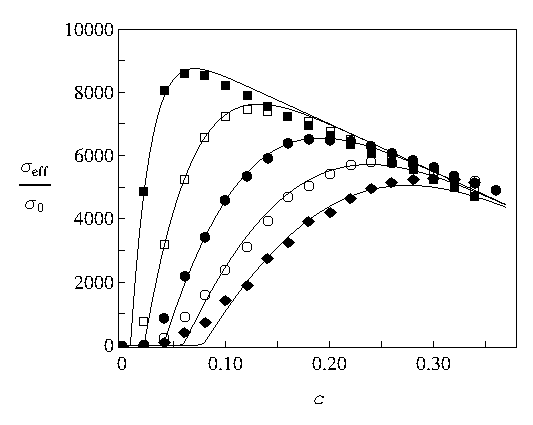
\includegraphics[width=\textwidth]{Fig6_Siekierski_HomogeneousLayers_t_fixed.eps}
		\caption{} \label{fig:simulations-sigma-1layer2005-a}
	\end{subfigure}
	\quad
	\begin{subfigure}[c]{0.48\textwidth}
		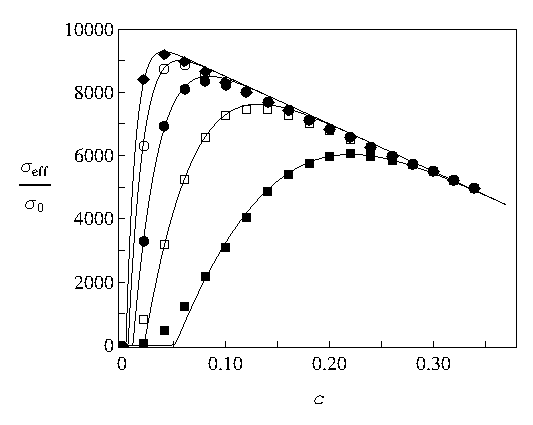
\includegraphics[width=\textwidth]{Fig7_Siekierski_HomogeneousLayers_d_fixed.eps}
		\caption{} \label{fig:simulations-sigma-1layer2005-b}
	\end{subfigure}
	\caption{\label{fig:simulations-sigma-1layer2005}
		Залежності ефективної провідності $\sigma_{\rm eff}$ від концентрації $c$, отримані в рамках симуляцій \cite{Siekierski2005} для частинок з електрично однорідними оболонками при (а) $h = 5$~мкм та $d = 3$ ($\blacksquare$), 5 ($\square$), 7 ($\bullet$), 9 ($\circ$) та 11 ($\blacklozenge$)~мкм; (б) $d = 5$~мкм та $h = 3$ ($\blacksquare$), 5 ($\square$), 7 ($\bullet$), 9 ($\circ$) та 11 ($\blacklozenge$)~мкм. 
		Неперервні лінії -- їх обробка за допомогою (\ref{eq:general_1layer_sigma}), (\ref{eq:phi_pen}) та (\ref{eq:K-delta-def}). 
		Використані параметри наведені в Таблиці~\ref{tab:numerical-homogeneous}}
\end{figure}

\begin{table}[t]
	\centering
	\caption{Параметри для обробки даних симуляцій, зображених на рис.~\ref{fig:simulations-sigma-1layer2005} за формулою (\ref{eq:general_1layer_sigma}).}
	\label{tab:numerical-homogeneous}
	\begin{tabular}{|l|l|r|r|r|r|r|}
		\hline
		\multirow{2}{*}{(а)} & $d$, мкм & 3 & 5 & 7 & 9 & 11 \\ \cline{2-7} 
		& $K/k$ & 1.0 & 1.05 & 1.05 & 1.07 & 1.10 \\ \hline
		\multirow{2}{*}{(б)} & $h$, мкм & 3 & 5 & 7 & 9 & 11 \\ \cline{2-7} 
		& $K/k$ & 1.08 & 1.05 & 1.06 & 1.07 & 1.06 \\ \hline
	\end{tabular}
\end{table}


\subsubsection{Аналіз екстремальної поведінки провідності}%\hfill

Значення провідностей компонентів, що були використані в розглядуваних симуляціях (див. Таблицю~\ref{tab:RRN-exper-params}) є характерними для деяких типів композитних електролітів та підкоряються умові $\sigma_1 \ll \sigma_0 \ll \sigma_2$, яка дозволяє істотно спростити (\ref{eq:general_1layer_sigma}), переходячи до межі $\sigma_1 \to 0$:
\begin{equation}\label{eq:sigma1to0}
4\sigma_{\rm eff}^3  -2 \left[(2-3
\phi)\sigma_0-(1+3c-3\phi)\sigma_2\right] \sigma_{\rm eff}^2
-(2-3c) \sigma_0\sigma_2\sigma_{\rm eff}=0.
\end{equation}
Це рівняння має два фізично-змістовних розв'язки, з яких один -- тривіальний ($\sigma_{\rm eff} = 0$), а другий:
\begin{equation}\label{eq:sigma1to0_conductivity}
\begin{split}
\sigma_{\rm eff} =& \frac{3}{4} \left[ \left( \frac{2}{3} - \phi \right) \sigma_0 +
\left( \phi - c - \frac{1}{3} \right) \sigma_2 + \right. \\
&+ \left. \sqrt{\left[  \left( \frac{2}{3} - \phi \right) \sigma_0 +
	\left( \phi - c - \frac{1}{3} \right) \sigma_2 \right]^2 + \frac{4}{3} \left( \frac{2}{3} - c \right) \sigma_0\sigma_2} \right].
\end{split}
\end{equation}
Для серій експериментів \cite{Siekierski2005} (рис.~\ref{fig:simulations-sigma-1layer2005}) графіки залежностей $\sigma_{\rm eff}$ від $c$, розраховані за (\ref{eq:general_1layer_sigma}) та (\ref{eq:sigma1to0_conductivity}), не відрізняються.

Положення максимуму провідності $c_{\rm max}$ знаходиться з наступних умов 
\begin{equation}\label{eq:max-conds}
	\left. \frac{\partial \sigma_{\rm eff}}{\partial c} \right|_{c = c_{\rm max}} = 0; \qquad
	\left. \frac{\partial^2 \sigma_{\rm eff}}{\partial c^2}\right|_{c = c_{\rm max}} < 0.
\end{equation}
Біля максимуму виконується $\sigma_{\rm eff} \sim \sigma_2 \gg \sigma_0$, тож рівняння (\ref{eq:sigma1to0_conductivity}) можна спростити:
\begin{equation}\label{eq:sigma1to0_conductivity-max}
 \sigma_{\rm eff} \approx \frac{3}{2} \left( \phi - c - \frac{1}{3} \right) \sigma_2,
\end{equation}
звідки перша з (\ref{eq:max-conds}) умов на положення максимуму $c_{\rm max}$ набирає вигляд:
\begin{equation}  \label{eq:maximumLocation}
\left. \frac{\partial \phi(c,\delta)}{\partial c}\,\right|_{c = c_{\rm
		{max}}} = 1.
\end{equation}
Цю умову можна сприймати як необхідну умову існування екстремуму об'єм\-ної концентрації оболонок $\phi - c$. Через те, що остання є неперервною невід'ємною функцією від $c$ та для проникних оболонок набирає нульові значення на границях її області визначення $c \in [0,1]$, шуканий екстремум відповідає її максимуму, а похідні $\partial^2\sigma_{\rm eff}/\partial c^2$ та $\partial^2\phi / \partial c^2$ мають однаковий знак у точці $c = c_{\rm max}$. 

На рис.~\ref{fig:simulations-max-1layer2005} представлено обробки даних симуляцій \cite{Siekierski2005} для залежностей $c_{\rm max}$ та $\sigma_{\rm max} = \sigma_{\rm eff}|_{c_{\rm max}}$ від $c$ за  співвідношеннями (\ref{eq:maximumLocation}) та (\ref{eq:sigma1to0_conductivity}), відповідно. Отримані теоретичні результати дуже добре узгоджуються з даними симуляцій, що відображає внутрішню послідовність приведеної процедури обробки даних.

\begin{figure}[tb]
	\centering
	\begin{subfigure}[c]{0.45\textwidth}
		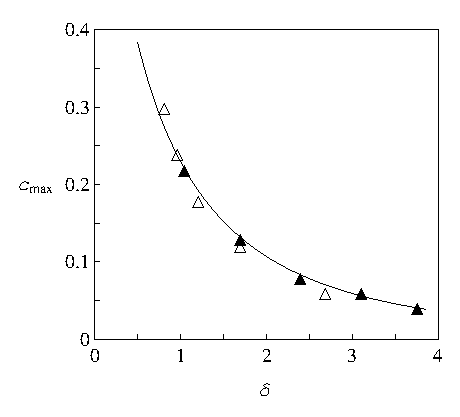
\includegraphics[width=\textwidth]{Siekierski_MaximumLocation.eps}
		\caption{} \label{fig:simulations-max-1layer2005-a}
	\end{subfigure}
	\quad
	\begin{subfigure}[c]{0.51\textwidth}
		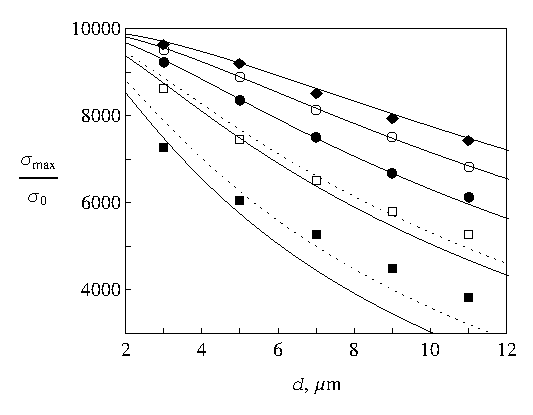
\includegraphics[width=\textwidth]{Siekierski_MaxConductivity.eps}
		\caption{} \label{fig:simulations-max-1layer2005-b}
	\end{subfigure}
	\caption{\label{fig:simulations-max-1layer2005} 
		Залежності \cite{Siekierski2005} (а) положення максимуму провідності $c_{\rm max}$ від $\delta$, взяті з даних на рис.~\ref{fig:simulations-sigma-1layer2005-a} ($\vartriangle$) та \ref{fig:simulations-sigma-1layer2005-b} ($\blacktriangle$), та (б) значення $\sigma_{\rm eff}|_{c_{\rm c}}$ в цій точці від $d$ при фіксованих $\sigma_2$ та $h = 3$ ($\blacksquare$), 5 ($\square$), 7 ($\bullet$), 9 ($\circ$) та 11 ($\blacklozenge$)~мкм (див. рис.~\ref{fig:simulations-sigma-1layer2005}); неперервні лінії -- їх обробки за (\ref{eq:maximumLocation}), (\ref{eq:sigma1to0_conductivity}),  (\ref{eq:phi_pen}) та (\ref{eq:K-delta-def}) при $K=k$ (точкові лінії -- те ж саме для $h = 3$ та 5~мкм при $K/k = 1.15$ та 1.07, відповідно)}
\end{figure}

\subsubsection{Випадок неоднорідних оболонок}

На рис. \ref{fig:simulations-sigma-Glayer2006} представлено обробки даних симуляцій \cite{Siekierski2006} для концентраційних залежностей $\sigma_{\rm eff}$ систем частинок з гаусовим профілем електричної провідності оболонок при різних значеннях їх товщин та діаметрів ядер. Використовуючи для розрахунків профіль $\sigma_2(u)$ виду (\ref{eq:GaussianProfile}), за допомогою (\ref{eq:general_Contlayer_sigma}), (\ref{eq:phi_pen}) та (\ref{eq:K-delta-def}) вдається відновити весь спектр симуляцій {\color{violet}із середньою середньоквадратичною відносною похибкою $\approx 0.092$ при $c > c_{\rm c}$
(максимальна середньоквадратична похибка дорівнює $\approx 0.54$ для $h=5$~мкм та $d=3$~мкм ($\blacksquare$) на рис.~\ref{fig:simulations-sigma-Glayer2006-b})}.
Зазначимо, що у випадках $h = 9$~мкм ($n = 18$) та $h = 11$~мкм ($n = 22$) з найбільшою кількістю комірок, припадаючих на оболонку, рівняння (\ref{eq:sigma-maxmin-rel}) дає, відповідно, $\log_{10} (\sigma'_{\rm max}/\sigma'_{\rm min}) = 2(n-2)/n \approx 1.78$ та 1.82  ($\sigma_{\rm max}/\sigma_{\rm min} = 100$). Ці дані відрізняються від отриманих з підгонки (див. Таблицю~\ref{tab:numerical-inhomogeneous-1}) не більш ніж на 17 та 12\%, відповідно. 

\begin{figure}[tb]
	\centering
	\begin{subfigure}[c]{0.48\textwidth}
		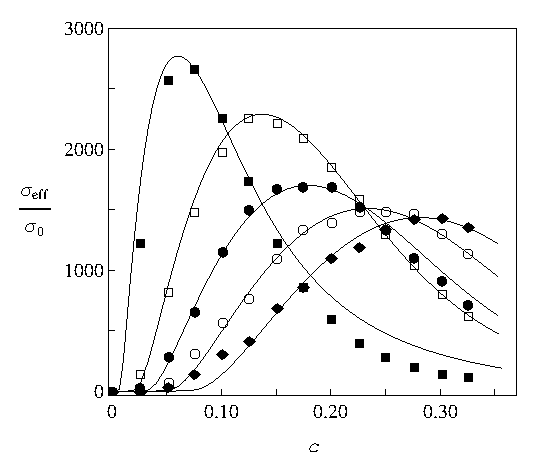
\includegraphics[width=\textwidth]{Siekierski_t_fixed.eps}
		\caption{} \label{fig:simulations-sigma-Glayer2006-a}
	\end{subfigure}
	\quad
	\begin{subfigure}[c]{0.48\textwidth}
		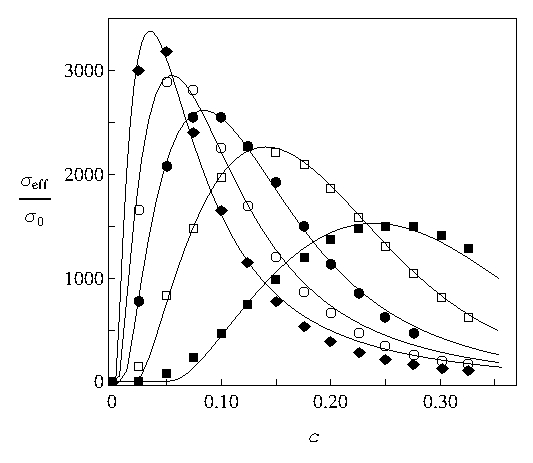
\includegraphics[width=\textwidth]{Siekierski_d_fixed.eps}
		\caption{} \label{fig:simulations-sigma-Glayer2006-b}
	\end{subfigure}
	\caption{\label{fig:simulations-sigma-Glayer2006} Залежності ефективної статичної провідності $\sigma_{\rm eff}$ від концентрації $c$, отримані в рамках симуляцій \cite{Siekierski2006} для частинок з профілем провідності оболонок гаусового типу при (а) $h = 5$~мкм та $d = 3$ ($\blacksquare$), 5 ($\square$), 7 ($\bullet$), 9 ($\circ$) та 11 ($\blacklozenge$)~мкм; (б) $d = 5$~мкм та $h = 3$ ($\blacksquare$), 5 ($\square$), 7 ($\bullet$), 9 ($\circ$) та 11 ($\blacklozenge$)~мкм. Неперервні лінії -- їх обробка в рамках профілю (\ref{eq:GaussianProfile}) та (\ref{eq:general_Contlayer_sigma}), (\ref{eq:phi_pen}), (\ref{eq:K-delta-def}), (\ref{eq:sigma-maxmin-rel}). Використані параметри наведені в Таблиці~\ref{tab:numerical-inhomogeneous-1}}
\end{figure}

\begin{table}[htb]
	\caption{\label{tab:numerical-inhomogeneous-1} Використані параметри для обробки даних симуляцій, зображених на рис.~\ref{fig:simulations-sigma-Glayer2006}, за формулою (\ref{eq:general_Contlayer_sigma}) з Гаусовим профілем  (\ref{eq:GaussianProfile}) оболонок при $\sigma'_{\rm min} = \sigma_{\rm min}$, $\sigma_0 = 10^{-8}$~См/см, $\sigma_1 = 10^{-12}$~См/см.}
	\begin{center}
		\begin{tabular}{|l|l|r|r|r|r|r|}
			\hline
			\multirow{3}{*}{(а)} & $d$, мкм & 3    & 5    & 7     & 9     & 11    \\ \cline{2-7}
			& $K/k$    & 1.09 & 1.02 & 1.13  & 1.11  & 1.09   \\ 
			\cline{2-7}
			& ${\rm log_{10}}\left(\sigma'_{\rm max}/\sigma'_{\rm min}\right)$
			& 1.83 & 1.89 & 1.82 & 1.88 & 1.98\\
			\hline
			\multirow{3}{*}{(б)} & $h$, мкм & 3    & 5    & 7     & 9     & 11    \\ \cline{2-7}
			& $K/k$    & 1.00  & 1.00  & 1.05 & 1.07 & 1.13  \\ \cline{2-7}
			& ${\rm log_{10}}\left(\sigma'_{\rm max}/\sigma'_{\rm min}\right)$
			& 1.90  & 1.89  & 1.85 & 1.85 & 1.87 \\
			\hline
		\end{tabular}
	\end{center}
\end{table}

Успішне тестування на числових даних симуляцій RRN дозволяє перейти до перевірки застосовності теорії для аналізу експериментальних даних для реальних систем. 


\section{Застосування моделі до опису концентраційної залежності  електричної провідності ТКЕ}\label{sec:CSE}

Спочатку розглянемо експериментальні дані для ефективної квазістатичної провідності ТКЕ $\rm LiI-Al_2O_3$ отримані  Ліангом~\cite{Liang1973}, який одним з перших продемонстрував можливість отримання немонотонного характеру $\sigma_{\rm eff}$ в таких системах.
Для виготовлення експериментальних зразків ТКЕ $\rm LiI-Al_2O_3$, спершу, суміші різних співвідношень порошків безводного $\rm LiI$ та $\rm Al_2O_3$, висушеного при $\rm 600^{o}C$, перемішувались, запікались при $\rm 550^{o}C$ приблизно 17 годин, гасились до кімнатної температури та дробились. Все це виконувалось в сухій ємності, заповненій гелієм (вміст $\rm H_2O$ та $\rm O_2$ складав менше ніж 15~г/м$^3$). Далі зважена кількість порошку $\rm LiI-Al_2O_3$ пресувалась до гранули у стальній ємності під тиском 690~МПА. Діаметр отриманої гранули дорівнював приблизно 1~мкм. До обох боків гранули були підключені літієві електроди зі стальними колекторами. Вимірювання шуканої ефективної провідності $\sigma_{\rm eff}$ отриманої комірки проводились при 1~кГц. 


\subsection{Процедура обробки експериментальних даних}

На першому етапі, обробка експериментальних даних виконується в рамках рівняння (\ref{eq:general_Contlayer_sigma}) зі ступінчатим профілем провідності (що відповідає моделі багатошарової оболонки; див. рис.~\ref{fig:model-Mlayers}), кількість ділянок в якому поступово збільшується доки не будуть отримані достатньо добрі результати. Зокрема, для обробки даних ТКЕ $\rm LiI-Al_2O_3$ були використані  профілі ${z}_2 (u) = \sigma_2 (u)/\sigma_0$ одношарової (однорідної) та двошарової оболонок, які у безрозмірних змінних ${z}_{2,i} = \sigma_{2,i}/\sigma_0$, $z_1 = \sigma_1/\sigma_0$, $z_0 = 1$ можуть бути записані наступним чином, використовуючи ступінчату функцію Хевісайда $\theta$:
\begin{enumerate}[leftmargin=*, label={\alph*)}]
	\item для однорідної оболонки:
	\begin{equation}\label{eq:profilex2-uniform}
	{z}_2 (u) = {z}_{2,1} + (1 - {z}_{2,1}) \theta(u - \delta_1),
	\end{equation}
	що відповідає рішенню (\ref{eq:sigma1to0_conductivity}) у термінах введених безрозмірних змінних при ${z}_{2,1} = {z}_2$;
	
	\item для ступінчатого профілю двошарової оболонки (рис. \ref{fig:model-2layers}):
	\begin{equation}\label{eq:profilex2-double}
	\begin{split}
	{z}_2 (u) = {z}_{2,1} +
	%+ \sum\limits_{i=1}^{M-1} ({z}_{2,i+1} - {z}_{2,i}) \theta(u-\delta_i) +(1 - {z}_{2,M}) \theta(u - \delta_M),
	({z}_{2,2} - {z}_{2,1}) \theta(u - \delta_1) + (1 - {z}_{2,2}) \theta(u - \delta_2),
	\end{split}
	\end{equation}
	що дає рівняння (\ref{eq:general_Mlayer_complex}) у безрозмірних змінних для ${z}_{\rm eff}$ при $M=2$.
\end{enumerate}

\begin{figure}[!ht]
	\centering
	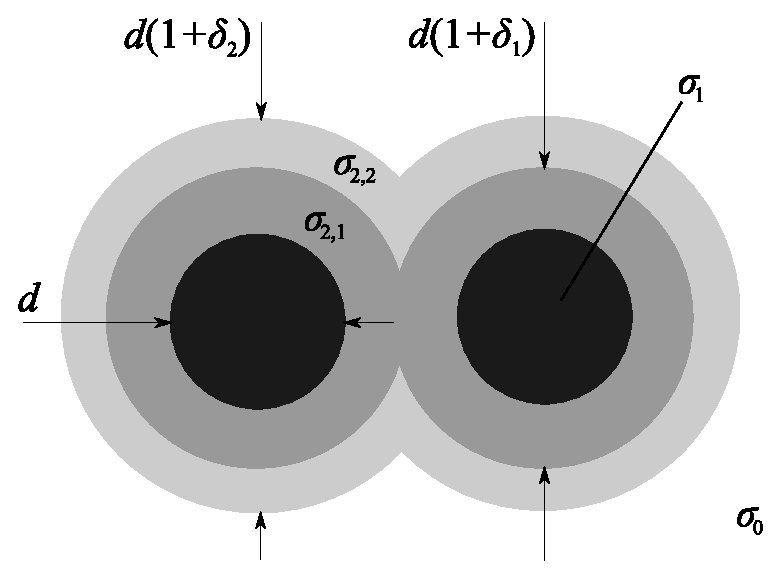
\includegraphics[width=0.55\textwidth]{model-2layer-sigma.eps}
	\caption{\label{fig:model-2layers} Модель системи частинок, що складаються з ядер (чорні області) радіусом $R_1 = d/2$ та провідністю $\sigma_{1}$ та двох концентричних шарів (сірі області), що мають провідності $\sigma_{2,1}$, $\sigma_{2,2}$ та товщини $h_1 = R_1\delta_1$, $h_2 = R_1(\delta_2 - \delta_1)$, відповідно}
\end{figure}

Ступінчатий профіль (\ref{eq:profilex2-double}) можна розглядати, як сукупність послідовних концентричних однорідних оболонок навколо ядра (див. рис.~\ref{fig:model-2layers}). Кожна $i$-та оболонка утворює перколяційний кластер при концентрації $c = c_{{\rm c},i}$, що знаходиться із рівняння (\ref{eq:threshold}) для $\delta_i$ (див. розділ \ref{sec:perc-analysis-threshold}), та має максимальний об'ємний внесок при концентрації $c = c_{{\rm m},i}$, яка визначається з рівняння 
$$
\left. \frac{\partial }{\partial c} (\phi(c,\delta_{i}) - \phi(c,\delta_{i-1})) \right|_{c_{{\rm m},i}} = 0 
\qquad (\phi(c, \delta_0) = c).
$$
Ефективна провідність ${z}_{\rm eff}$ зростає на проміжку $(c_{{\rm c},i}; c_{{\rm m},i})$, якщо провідність ${z}_{2,i}$ цієї оболонки більша ніж провідність ${z}_{2,i+1}$ наступної більш далекої від ядра оболонки; якщо ${z}_{2,i} < {z}_{2,i+1}$, то ${z}_{\rm eff}$ спадає. Для найбільш далекої від ядра оболонки ($i=M$) поведінка ${z}_{\rm eff}$ на проміжку $(c_{{\rm c},M}; c_{{\rm m},M})$ визначається співвідношенням між ${z}_{2,M}$ та ${z}_0 = 1$.
На проміжку $(c_{{\rm m},i}; c_{{\rm c},i-1})$ ефективна відносна провідність ${z}_{\rm eff}$ зростає, якщо ${z}_{2,i} < {z}_{2,i-1}$, та спадає у протилежному випадку. Для найбільш близької до ядра оболонки ($i=1$) поведінка $z_{\rm eff}$ визначається відношенням між ${z}_{2,1}$ та ${z}_1$ на проміжку $(c_{{\rm m},1}; c'_{{\rm c}})$, де $c_{\rm c}' = 1/3$ -- поріг перколяції для твердих ядер частинок в рамках МКГ (див. розділ \ref{sec:double-perc}).
Використовуючи ці твердження за індукцією для кожної оболонки, концентраційний інтервал $(c_{{\rm c},M}, 1/3)$ для ступінчатого $M$-шарового профілю можна розбити на $M$ проміжків: 
$$
(c_{{\rm c},M}, 1/3) \simeq \bigcup\limits_{i=1}^M (c_{{\rm c},i}, c_{{\rm c},i-1}), \quad c_{{\rm c},0} = c'_{\rm c} = 1/3,
$$ 
на кожному з яких ${z}_{\rm eff}$: а) має максимум при $c=c_{{\rm m},i}$ ($c_{{\rm c},i} < c_{{\rm m},i} < c_{{\rm c},i-1}$), якщо ${z}_{2,i+1}, {z}_{2,i-1} < {z}_{2,i}$ (${z}_{2,M+1} = {z}_0$; ${z}_{2,0} = {z}_1$), та мінімум у протилежному випадку; б) монотонно зростає, якщо ${z}_{2,i-1} > {z}_{2,i} > {z}_{2,i+1}$, та спадає у протилежному випадку. Зазначимо, що така екстремальна поведінка ${z}_{\rm eff}$ помітна лише для достатньо товстих оболонок з істотною різницею провідностей сусідніх областей.

Такий зв'язок між значеннями провідностей ${z}_{2,i}$ частин оболонки та поведінкою ${z}_{\rm eff}$ на відповідних концентраційних інтервалах дозволяє аналізувати внески різних ефектів та механізмів, домінуючих на цих інтервалах. Зокрема, в дисертаційній роботі вважається, що якщо різниця між провідностями сусідніх оболонок істотна, ці оболонки відображають різні ефекти.
%\end{enumerate}

Гладкий профіль є більш послідовним, з фізичної точки зору, ніж ступінчатий, тому далі профіль (\ref{eq:profilex2-double}) згладжувався суперпозицією сигмоїд:
\begin{equation}\label{eq:profilex2-sigmoid2}
\begin{split}
{z}_2 (u) = {Z}_{2,1} 
%+ \sum\limits_{i=1}^{M-1} \frac{{Z}_{2,i+1} - {Z}_{2,i}}{1 + \exp{\left( - \frac{u - \Delta_i}{\alpha} \right)}} + \frac{1 - {Z}_{2,M}}{1 + \exp{\left( - \frac{u - \Delta_M}{\alpha} \right)}},
+ \frac{{Z}_{2,2} - {Z}_{2,1}}{1 + \exp{\left( - \frac{u - \Delta_1}{\alpha} \right)}}  + \frac{1 - {Z}_{2,2}}{1 + \exp{\left( - \frac{u - \Delta_2}{\alpha} \right)}},
\end{split}
\end{equation}
де ${Z}_{2,i}$, $\Delta_{i}$ та $\alpha$ виступають в ролі параметрів функції профілю оболонки. У наближенні $\alpha \to 0$ параметри ${Z}_{2,i}$, $\Delta_{i}$ прямують до ${z}_{2,i}$ та $\delta_i$, відповідно, а рівняння (\ref{eq:profilex2-sigmoid2}) набирає вигляд (\ref{eq:profilex2-double}). 

Всі параметри оболонок вважаються підгінними.

\subsection{Результати обробки}

Результати обробки даних \cite{Liang1973} представлені на рис.~\ref{fig:Liang_LiI-Al2O3-Processing} та у Таблиці~\ref{tab:Liang}. 
Добре відновити дані {\color{violet}(з середньоквадратичною відносною похибкою $\approx 0.15$)}  вдається використовуючи моделі зі ступінчатою (\ref{eq:profilex2-double}) та неперервною (\ref{eq:profilex2-sigmoid2}) оболонками (штрихована та неперервна лінії, відповідно).
Модель з електрично однорідною оболонкою (\ref{eq:profilex2-uniform}) не відновлює дані в області $c \lesssim 0.3$ (точкова лінія).

\begin{figure}[!ht]
	\centering
	\begin{subfigure}[b]{0.48\textwidth}
		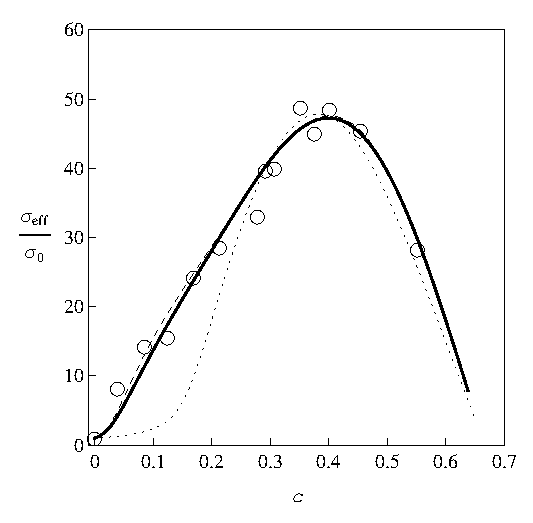
\includegraphics[width=\textwidth]{Fig12_Liang_LiI-Al2O3-Processing.eps}
		\caption{} \label{fig:Liang_LiI-Al2O3-Processing-a}
	\end{subfigure}
	\quad
	\begin{subfigure}[b]{0.48\textwidth}
		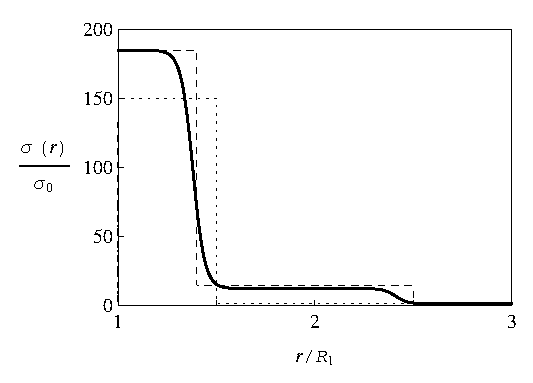
\includegraphics[width=\textwidth]{Fig13_Liang_LiI-Al2O3-Profile.eps}
		\caption{} \label{fig:Liang_LiI-Al2O3-Processing-b}
	\end{subfigure}
	\caption{\label{fig:Liang_LiI-Al2O3-Processing} 
		(а) Залежність ${z}_{\rm eff}$ від $c$ для ТКЕ $\rm{LiI-Al_2O_3}$ \cite{Liang1973} та (б) використані для її обробки одночастинкові профілі провідності частинок: точкові лінії -- однорідний профіль (\ref{eq:profilex2-uniform}); штриховані лінії -- ступінчатий профіль (\ref{eq:profilex2-double}); неперервні лінії -- суперпозиція сигмоїд (\ref{eq:profilex2-sigmoid2}). Використані параметри приведені в Таблиці~\ref{tab:Liang}}
\end{figure}

\begin{table}[tb]
	\caption{\label{tab:Liang} Параметри, що використовувались для обробки
		даних \cite{Liang1973} з $\sigma_{\rm eff}$ для ТКЕ $\rm{LiI-Al_2O_3}$
		в рамках однорідної (\ref{eq:profilex2-uniform}), ступінчатої
		(\ref{eq:profilex2-double}), та сигмойдної (\ref{eq:profilex2-sigmoid2})
		моделей профілю ${z}_2(u)$ при ${z}_1 = 0$ та
		$\sigma_0 = 2.5 \times 10^{-7}$~См/см.}
	\begin{center}
		\begin{tabular}{|l|l|l|l|l|l|}
			\hline
			а) & ${z}_2$ & $\delta$ & &  &  \\
			& 150    & 0.5   &  &  & \\
			\hline
			б)  & ${z}_{2,1}$   &${z}_{2,2}$ & $\delta_1$ & $\delta_2$ &  \\
			& 185         & 14  & 0.40       & 1.50       &  \\
			\hline
			в)  & ${Z}_{2,1}$    &${Z}_{2,2}$    & $\Delta_1$ & $\Delta_2$ &  $\alpha$ \\
			& 185         & 12        & 0.38       & 1.41       &   0.03    \\
			\hline
		\end{tabular}
	\end{center}
\end{table}

Дальня від ядра частина отриманого профілю (див. рис.~\ref{fig:Liang_LiI-Al2O3-Processing-b}) починає грати роль при концентраціях $c_{{\rm c},2} \approx 0.025$. Тобто вже при досить малих концентраціях ядер майже весь матеріал матриці витісняється фазою дальньої частини оболонки. Це можна інтерпретувати наступним чином.
Формально рівняння (\ref{eq:general_Contlayer_sigma}) для $\sigma_{\rm eff}$ цієї системи з отриманим профілем (\ref{eq:profilex2-double}) можна представити у вигляді системи двох рівнянь у введених безрозмірних змінних:
\begin{equation}\label{eq:conductivityNewMatrix}
\left(1-\phi(c, \delta_1)\right)\frac{{z}^{*}_0(c) -{z}_{\rm
		eff}}{2{z}_{\rm eff}+{z}^{*}_0(c)} + c\,\frac{{z}_1
	-{z}_{\rm
		eff}}{2{z}_{\rm eff}+{z}_1} 
+\left(\phi(c, \delta_1)-c\right)\frac{{z}_{2,1} -{z}_{\rm
		eff}}{2{z}_{\rm eff}+{z}_{2,1}}=0,
\end{equation}
\begin{equation}\label{eq:sigma0-vs-c}
\begin{split}
(1 - \phi(c,\delta_1))\frac{{z}^{*}_0(c) - {z}_{\rm
		eff}}{2{z}_{\rm eff} + {z}^{*}_0(c)} =& (1 - \phi(c,\delta_2))
\frac{1 - {z}_{\rm eff}}{2{z}_{\rm eff} + 1}\\
&+ (\phi(c,\delta_2) - \phi(c,\delta_1)) \frac{{z}_{2,2} -
	{z}_{\rm eff}}{2{z}_{\rm eff} + {z}_{2,2}}.
\end{split}
\end{equation}
Можна вважати, що перше рівняння описує модельну систему з однорідним профілем (\ref{eq:profilex2-uniform}) оболонки, яка має провідність ${z}_{2,1}$ та відносну товщину $\delta_1$, та матрицею з провідністю ${z}^{*}_0$, що залежить від концентрації за законом, визначеним другим рівнянням. 
Ця залежність для параметрів отриманих для ТКЕ $\rm LiCl-Al_2O_3$~\cite{Liang1973} показана на рис.~\ref{fig:Liang_LiI-Al2O3-Matrix}. При відносно низьких концентраціях ($c \lesssim c_{{\rm c},1} \approx 0.126$) виконується ${z}_{\rm eff} \approx {z}^{*}_0$, тобто ${z}_{\rm eff}$ визначається тільки через параметри ${z}_{2,2}$ та $\delta_2$ зовнішньої частини ступінчатого профілю (\ref{eq:profilex2-double}); внутрішня частина останнього починає грати роль лише поблизу $c_{{\rm c},1}$. Тобто, можна вважати, що дальня від ядра частина отриманого двошарового профілю (рис. \ref{fig:Liang_LiI-Al2O3-Processing-b}) ефективно враховує залежність провідності матриці від концентрації частинок. 
\begin{figure}[tb]
	\centering
	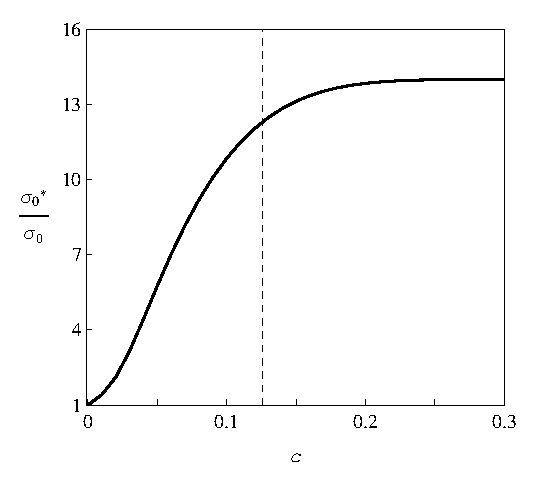
\includegraphics[width=0.55\textwidth]{Fig14_Liang_LiI-Al2O3-Matrix_2.eps}
	\caption{\label{fig:Liang_LiI-Al2O3-Matrix} Залежність провідності матриці ${z}^{*}_0$ від $c$ (неперервна лінія), згідно рівняння~(\ref{eq:sigma0-vs-c}) для ступінчатого профілю на рис.~\ref{fig:Liang_LiI-Al2O3-Processing-b} (див. Таблицю~\ref{tab:Liang}); штрихована лінія -- положення порогу перколяції $c_{{\rm c},1} \approx 0.126$ для внутрішньої оболонки}
\end{figure}
З фізичної точки зору, таку поведінку провідності матриці можуть викликати: формування поблизу поверхні частинок області просторового заряду за рахунок високої концентрації дефектів в полікристалічній матриці~\cite{Maier1986}; розвинення високопровідної мережі зв'язаних дислокацій, утворених механічним або термальним шляхом~\cite{Dudney1987, Dudney1988, Muhlherr1988}; швидкий іонний транспорт уздовж поверхні розділу матриця-частинки та/або дислокацій~\cite{Phipps1981, Atkinson1988}; однорідне допування матриці за рахунок розчинення неоднорідностей та малих частинок~\cite{Wen1983, Dupree1983, Dudney1985} тощо.

Висока провідність найближчої до ядра ділянки може бути викликана формуванням  області просторового заряду (великої концентрації точкових дефектів) за рахунок адсорбції (десорбції)~\cite{Jow1979}; швидким іонний транспортом уздовж границь частинка~-~матриця за рахунок пошкодження структури матриці~\cite{Phipps1981,Phipps1983}; стабілізацією провідних нерівноважних станів за рахунок прилеглих частинок~\cite{Ploch1988,Wiec1989}; формуванням нової ``суперструктури'' за рахунок хімічних реакцій у міжфазній області~\cite{Schmidt1988} тощо. Зокрема, для ТКЕ $\rm LiI-Al_2O_3$ отримані оцінки ($\delta_1 = 0.4$ та $x_{2,1} = 185$) задовольняють результатам \cite{Jiang1995a,Jiang1995b} ($\delta=0.4$, $x_2 = 324$), отриманим для кубічної ґратки з рівноважним розподілом частинок у припущенні, що висока провідність навколо останніх є наслідком утворення областей просторового заряду.


\section{Ефективна електрична провідність ПКЕ}

Зразки розглядуваних ПКЕ \cite{Przl1995, Wiec1994} виготовлялись наступним чином. Полімерна матриця та сіль розчинялись у ацетонітрилі, куди додавалися частинки дисперсної фази. Отримана суспензія перемішувалась до видимої однорідності та поміщалась на плоску скляну або тефлонову підкладку. Розчинник випарювався під вакуумом у вакуумному ексикаторі. Далі, отримані композити 48 годин висушувалися при температурі $\rm 60^{o}C$. PAAM отримувався полімеризацією акриламіда в ацетонітрильному розчині використовуючи пероксид бензолу, після чого він 48 годин висушувався при $\rm 100^{o}C$. 
Всі етапи проходили у наповненій аргоном сухій ємності.

Провідність зразків вимірювалась методами імпедансної спектроскопії у частотному проміжку від 5 Гц до 13 МГц. Мікроструктура зразків вивчалася методом рентгенівської дифрактометрії. Для отримання рівня кристалізованості використовували метод диференційної скануючої калориметрії.

%\subsection{Процедура обробки експериментальних даних}

Процедура обробки експериментальних даних з концентраційної залежності ${z}_{\rm eff}$ збігається з використаною у попередньому підрозділі, додатково розглядаючи ступінчатий профіль тришарової моделі та відповідну суперпозицію сигмоїд:
\begin{equation}\label{eq:profilex2-triple}
\begin{split}
{z}_2 (u) =& {z}_{2,1} +
%+ \sum\limits_{i=1}^{M-1} ({z}_{2,i+1} - {z}_{2,i}) \theta(u-\delta_i) +(1 - {z}_{2,M}) \theta(u - \delta_M),
({z}_{2,2} - {z}_{2,1}) \theta(u - \delta_1) + ({z}_{2,3} - {z}_{2,2}) \theta(u - \delta_2) +\\
&+ (1 - {z}_{2,3}) \theta(u - \delta_3);
\end{split}
\end{equation}
\begin{equation}\label{eq:profilex2-sigmoid3}
\begin{split}
{z}_2 (u) =& {Z}_{2,1} 
%+ \sum\limits_{i=1}^{M-1} \frac{{Z}_{2,i+1} - {Z}_{2,i}}{1 + \exp{\left( - \frac{u - \Delta_i}{\alpha} \right)}} + \frac{1 - {Z}_{2,M}}{1 + \exp{\left( - \frac{u - \Delta_M}{\alpha} \right)}},
+ \frac{{Z}_{2,2} - {Z}_{2,1}}{1 + \exp{\left( - \frac{u - \Delta_1}{\alpha} \right)}}  + \frac{{Z}_{2,3} - {Z}_{2,2}}{1 + \exp{\left( - \frac{u - \Delta_2}{\alpha} \right)}} +\\
&+ \frac{1 - {Z}_{2,3}}{1 + \exp{\left( - \frac{u - \Delta_3}{\alpha} \right)}}.
\end{split}
\end{equation}

\subsection{Результати обробки концентраційних залежностей}%\mbox{}

Результати обробки даних \cite{Przl1995, Wiec1994} для ПКЕ на основі PEO з частинками NASICON та $\rm \theta$-$\rm Al_2O_3$ представлені на рис.~\ref{fig:PEO-NaIa}; використані параметри та відповідні значення $R^2$ подано у таблицях~\ref{tab:adjustable_params-11} та \ref{tab:adjustable_params-12}. 
\begin{figure}[!t]
	\centering
	\begin{subfigure}[c]{0.54\textwidth}
		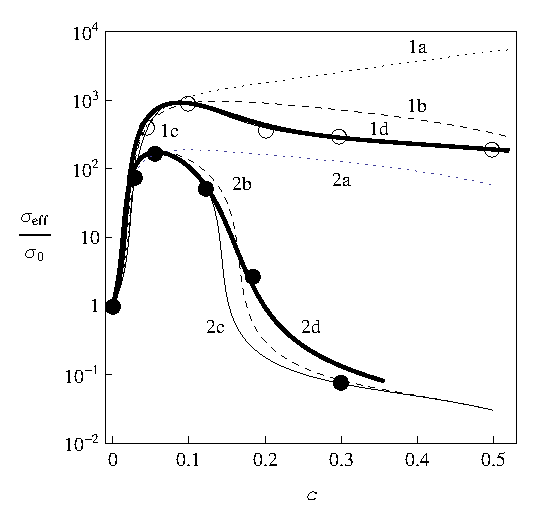
\includegraphics[width=\textwidth]{Fig2_PEO-NaI_NASICON_PEO-NaI-theta-Al2O3.eps}
		\caption{} \label{fig:PEO-NaIa}
	\end{subfigure}%
	~
	\begin{subfigure}[c]{0.45\textwidth}
		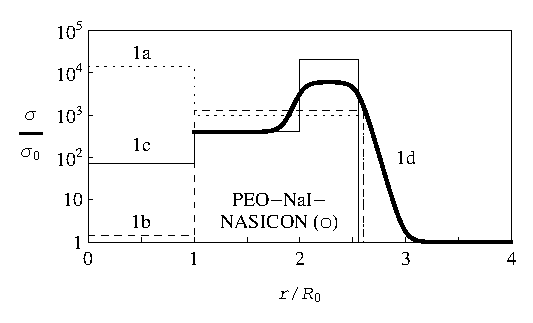
\includegraphics[width=\textwidth]{Fig2_PEO-NaI_NASICON_Profile.eps}
		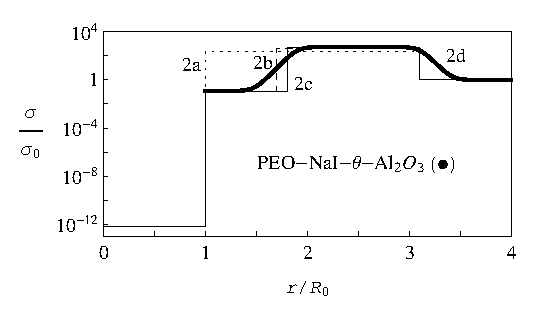
\includegraphics[width=\textwidth]{Fig2_PEO-NaI-theta-Al2O3_Profile.eps}
		\caption{} \label{fig:PEO-NaIb}
	\end{subfigure}
	\caption{\label{fig:PEO-NaI} (а) Залежності відносної ефективної провідності ${z}_{\rm eff}$ від об'ємної концентрації включень $c$ для ПКЕ PEO--NaI--NASICON ($\circ$) \cite{Przl1995} та (PEO)$_{10}$--NaI--$\theta$-Al$_2$O$_3$ ($\bullet$) \cite{Wiec1994}, та їх підгонки в рамках моделей однорідної (\ref{eq:profilex2-uniform}), двошарової (\ref{eq:profilex2-double}) та неперервної (\ref{eq:profilex2-sigmoid2}) оболонок. (б) Відповідні одночастинкові профілі провідності. Позначення вказують на використані з таблиць~\ref{tab:adjustable_params-11} та \ref{tab:adjustable_params-12} параметри}
\end{figure}
Для отримання достатньо добрих результатів {\color{violet}(мінімальне значення $R^2$ дорівнює 95\%)} необхідно використовувати ступінчату (\ref{eq:profilex2-double}) або неперервну (\ref{eq:profilex2-sigmoid2}) моделі двошарових оболонок (лінії 1c, 1d, 2b, 2c, 2d); модель (\ref{eq:profilex2-uniform}) однорідної оболонки (лінії 1a, 1b, 2a) не спроможна навіть якісно відновити шукані залежності. Для ПКЕ з включеннями PAAM \cite{Przl1995, Wiec1994} (див. рис.~\ref{fig:OMPEO-LiClO4}) потрібно використовувати ступінчатий профіль щонайменш тришарової оболонки (\ref{eq:profilex2-triple}) для отримання адекватних результатів {\color{violet}(найменше значення $R^2 \approx 92.3$\%)}.
%Максимуми цих залежностей знаходяться при значеннях $c$ від 0.05 до 0.1 для неорганічних включень та від 0.2 до 0.3 для органічних, з можливим мінімумом ${z}_{\rm eff}$ при значенні $c$ близького до 0.1 для OMPEO--LiClO$_4$--PAAM. 


\begin{table}[!tb]
	\centering \caption{\label{tab:adjustable_params-11} Параметри, що були
		використані для обробки даних \cite{Przl1995,Wiec1994} з 
		концентраційних залежностей для ПКЕ при $t= 25\,\rm{^oC}$ в 
		рамках моделей однорідної (\ref{eq:profilex2-uniform}), двошарової (\ref{eq:profilex2-double})
		та неперервних (\ref{eq:profilex2-sigmoid2}) оболонок та значення $R^2$
		для найкращих результатів.}
	\begin{threeparttable}
		\begin{tabularx}{\textwidth}{|X|l|X|l|l|l|l|l|}
			\hline
			\multirow{2}{*}{Оболонка} &\multirow{2}{*}{L\tnote{a}} &   \multirow{2}{*}{${z}_1$} & $\delta_1$\tnote{b} & $\delta_2$\tnote{b} &  ${z}_{21}$\tnote{b} & ${z}_{22}$\tnote{b} &  \multirow{2}{*}{$R^2$, \%} \\
			&  & & $\Delta_1$\tnote{c}& $\Delta_2$\tnote{c}&${Z}_{21}\tnote{c}$&${Z}_{22}$\tnote{c}& \\
			\hline
			\multicolumn{8}{c}{PEO--NaI--NASICON ($\sigma_0 \approx 9.86\times 10^{-9}$~См/см)}\\
			\hline
			однорідна  &1a   & $1.4\times 10^4$ &1.6& -- &  1000& -- & --  \\
			однорідна                 &1b                                       &1.4             &1.6& -- &  1300& -- & -- \\
			подвійна                 &1c                                       &70              &1.0&1.55&  400  &  20000  &  99.4 \\
			неперервна, &1d                   &70              &1.0&1.55&  400 &  6000  &  95.5 \\
			$\alpha =0.05$ &    & & & &  & &  \\
			\hline
		\end{tabularx}
		\begin{tablenotes}
			\item[a] Використані позначення для підгонок на відповідних
			рисунках.
			\item[b] Параметри для моделей дискретних оболонок.
			\item[c] Параметри для моделей неперервних оболонок.
		\end{tablenotes}
	\end{threeparttable}
\end{table}


\begin{table}[!tb]
	\centering \caption{\label{tab:adjustable_params-12} Параметри, що були
		використані для обробки даних \cite{Przl1995,Wiec1994} з 
		концентраційних залежностей для ПКЕ при $t= 25\,\rm{^oC}$ в 
		рамках моделей однорідної (\ref{eq:profilex2-uniform}), двошарової (\ref{eq:profilex2-double})
		та неперервних (\ref{eq:profilex2-sigmoid2}) оболонок та значення $R^2$
		для найкращих результатів.}
	\begin{threeparttable}
		\begin{tabularx}{\textwidth}{|X|l|X|l|l|l|l|l|}
			\hline
			\multirow{2}{*}{Оболонка} &\multirow{2}{*}{L\tnote{a}} &   \multirow{2}{*}{${z}_1$} & $\delta_1$\tnote{b} & $\delta_2$\tnote{b} &  ${z}_{21}$\tnote{b} & ${z}_{22}$\tnote{b} &  \multirow{2}{*}{$R^2$, \%} \\
			&  & & $\Delta_1$\tnote{c}& $\Delta_2$\tnote{c}&${Z}_{21}\tnote{c}$&${Z}_{22}$\tnote{c}& \\
			\hline
			\multicolumn{8}{c}{(PEO)$_{10}$--NaI--$\theta$-Al$_2$O$_3$ ($\sigma_0 \approx 1.54\times 10^{-8}$~См/см)}\\
			\hline
			однорідна &2a & \multirow{5}{*}{$6.5\times 10^{-13}$} &2.1&--&230&--&--  \\
			подвійна &2b                                       &                   &0.7&2.1&0.12&435& 92.8\\
			подвійна &2c                                       &                   &0.8&2.1&0.12&520& 98.6\\
			неперервна, &2d                                  &                   &0.9&2.1&0.12&560& 95.0\\
			$\alpha =0.05$  &  & & & & & &   \\
			\hline
		\end{tabularx}
		\begin{tablenotes}
			\item[a] Використані позначення для підгонок на відповідних
			рисунках.
			\item[b] Параметри для моделей дискретних оболонок.
			\item[c] Параметри для моделей неперервних оболонок.
		\end{tablenotes}
	\end{threeparttable}
\end{table}

\begin{figure*}[tb]
	\centering
	\begin{subfigure}[c]{0.54\textwidth}
		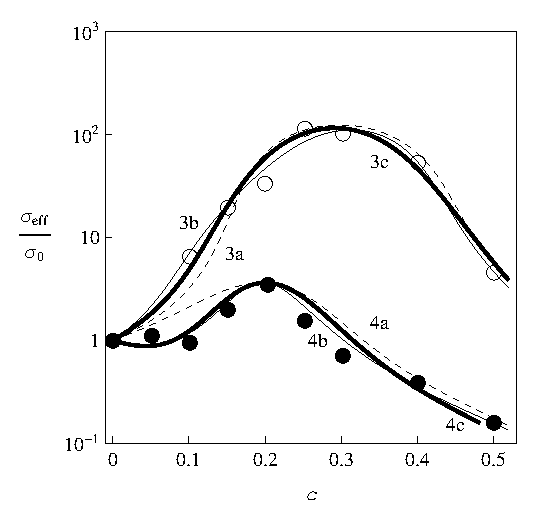
\includegraphics[width=\textwidth]{Fig3_PEO-PAAM_LiClO4_OMPEO-PAAM_LiClO4.eps}
		\caption{} \label{fig:OMPEO-LiClO4a}
	\end{subfigure}%
	~
	\begin{subfigure}[c]{0.45\textwidth}
		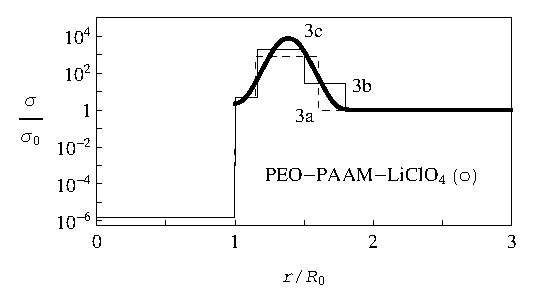
\includegraphics[width=\textwidth]{Fig3_PEO-PAAM_LiClO4_Profile.eps}
		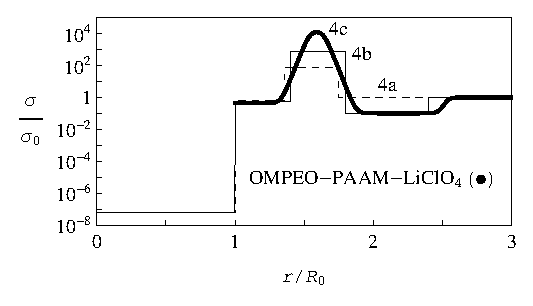
\includegraphics[width=\textwidth]{Fig3_OMPEO-PAAM_LiClO4_Profile.eps}
		\caption{} \label{fig:OMPEO-LiClO4b}
	\end{subfigure}
	\caption{\label{fig:OMPEO-LiClO4} (а) Залежності відносної ефективної провідності ${z}_{\rm eff}$ від об'ємної концентрації включень $c$ для ПКЕ PEO--LiClO$_4$--PAAM ($\circ$)
		\cite{Przl1995, Wiec1994} та OMPEO--LiClO$_4$--PAAM ($\bullet$) \cite{Wiec1994}, та їх підгонки в рамках моделей двошарової (\ref{eq:profilex2-double}), тришарової (\ref{eq:profilex2-triple}) та неперервної (\ref{eq:profilex2-sigmoid3}) оболонок. (б) Відповідні одночастинкові профілі провідності. Позначення вказують на використані з таблиць~\ref{tab:adjustable_params-21} та \ref{tab:adjustable_params-22} параметри}
\end{figure*}

\begin{table}[!htb]
	\centering \caption{\label{tab:adjustable_params-21} Параметри, що були
		використані для обробки даних \cite{Przl1995,Wiec1994} з 
		концентраційних залежностей для ПКЕ при $t= 25\,\rm{^oC}$ в 
		рамках моделей двошарової (\ref{eq:profilex2-double}), тришарової (\ref{eq:profilex2-triple}) 
		та неперервної 
		(\ref{eq:profilex2-sigmoid3}) оболонок та значення $R^2$
		для найкращих результатів.}
	\begin{threeparttable}
		\begin{tabularx}{\textwidth}{|X|l|X|l|l|l|l|l|l|l|}
			\hline
			\multirow{2}{*}{Оболонка} &\multirow{2}{*}{L\tnote{a}} &   \multirow{2}{*}{${z}_1$} & $\delta_1$\tnote{b} & $\delta_2$\tnote{b} & $\delta_3$\tnote{b} & ${z}_{21}$\tnote{b} & ${z}_{22}$\tnote{b} & ${z}_{23}$\tnote{b} & \multirow{2}{*}{$R^2$, \%} \\
			&  & & $\Delta_1$\tnote{c}& $\Delta_2$\tnote{c}&$\Delta_3$\tnote{c}&${Z}_{21}\tnote{c}$&${Z}_{22}$\tnote{c}&${Z}_{23} \tnote{c}$ & \\
			\hline
			\multicolumn{10}{c}{PEO--LiClO$_4$--PAAM ($\sigma_0 \approx 6.12\times 10^{-7}$~См/см)}\\
			\hline
			подвійна &3a & \multirow{4}{*}{$1.6\times 10^{-6}$} &0.15&0.60& -- & 5.0           &800 &--& 88.7 \\
			потрійна  &3b                                     &                  &0.16&0.50&0.80 & 5.0 &1800 &27 &  92.3 \\
			неперервна,  &3c                      &                   &0.32&0.45&0.48 & 2.0     &9400&27 & 92.9 \\
			$\alpha =0.03$ &   & & & & & &  & & \\
			\hline
		\end{tabularx}
		\begin{tablenotes}
			\item[a] Використані позначення для підгонок на відповідних
			рисунках.
			\item[b] Параметри для моделей дискретних оболонок.
			\item[c] Параметри для моделей неперервних оболонок.
		\end{tablenotes}
	\end{threeparttable}
\end{table}

\begin{table}[!htb]
	\centering \caption{\label{tab:adjustable_params-22} Параметри, що були
		використані для обробки даних \cite{Przl1995,Wiec1994} з 
		концентраційних залежностей для ПКЕ при $t= 25\,\rm{^oC}$ в 
		рамках моделей двошарової (\ref{eq:profilex2-double}), тришарової (\ref{eq:profilex2-triple}) 
		та неперервної 
		(\ref{eq:profilex2-sigmoid3}) оболонок та значення $R^2$
		для найкращих результатів.}
	\begin{threeparttable}
		\begin{tabularx}{\textwidth}{|X|l|X|l|l|l|l|l|l|l|}
			\hline
			\multirow{2}{*}{Оболонка} &\multirow{2}{*}{L\tnote{a}} &   \multirow{2}{*}{${z}_1$} & $\delta_1$\tnote{b} & $\delta_2$\tnote{b} & $\delta_3$\tnote{b} & ${z}_{21}$\tnote{b} & ${z}_{22}$\tnote{b} & ${z}_{23}$\tnote{b} & \multirow{2}{*}{$R^2$, \%} \\
			&  & & $\Delta_1$\tnote{c}& $\Delta_2$\tnote{c}&$\Delta_3$\tnote{c}&${Z}_{21}\tnote{c}$&${Z}_{22}$\tnote{c}&${Z}_{23} \tnote{c}$ & \\
			\hline
			\multicolumn{10}{c}{OMPEO--LiClO$_4$--PAAM, після отжигу ($\sigma_0 \approx 1.61\times 10^{-5}$~См/см)}\\
			\hline
			подвійна   &4a  & \multirow{4}{*}{$6.2\times 10^{-8}$} &0.36&0.75& -- &0.60& 75 &--& 46.3\\
			потрійна   & 4b                  &                    &0.40&0.80&1.40&0.57& 750&0.10 &  93.8\\
			неперервна, &4c                     &                    &0.54&0.64&1.53&0.44&14200&0.10 &  81.7\\
			$\alpha =0.02$ &  &  & & & & &  & & \\
			\hline
		\end{tabularx}
		\begin{tablenotes}
			\item[a] Використані позначення для підгонок на відповідних
			рисунках.
			\item[b] Параметри для моделей дискретних оболонок.
			\item[c] Параметри для моделей неперервних оболонок.
		\end{tablenotes}
	\end{threeparttable}
\end{table}

Використання моделі неперервної оболонки дає змогу отримати форму профілю провідності оболонки (див. рис.~\ref{fig:PEO-NaIb}, \ref{fig:OMPEO-LiClO4b}, неперервні лінії) дуже схожу на використаний в розділі~\ref{sec:CSE} гаусів профіль (\ref{eq:GaussianProfile}).
Однак, для розглянутих ПКЕ такі профілі не призводять до значного покращення результатів для ${z}_{\rm eff}$ у порівнянні зі ступінчатим профілем {\color{violet}(див. значення $R^2$ в таблицях~\ref{tab:adjustable_params-11}, \ref{tab:adjustable_params-12}, \ref{tab:adjustable_params-21}, \ref{tab:adjustable_params-22})}.

Отримані ступінчаті профілі свідчать про наявність двох (для неорганічних включень) та трьох (для органічних) чітко виражених ділянок (див. рис.~\ref{fig:PEO-NaIb}, \ref{fig:OMPEO-LiClO4b}). 
Центральна ділянка ${z}_2(u)$ (дальня, для двошарової моделі) характеризується провідністю, що на кілька порядків перевищує провідність матриці. Цей результат узгоджується з експериментально перевіреним фактом \cite{nanocomp2008} про формування навколо частинок в ПКЕ аморфізованих областей з відносно високою провідністю, яка є результатом підвищеної сегментарної гнучкості полімерних ланцюгів та, відповідно, підвищеної рухливості іонів розчиненої солі в цих областях. 

Найближча до ядер  ділянка ${z}_2(u)$ описує сумарний ефект кількох можливих процесів: затруднення руху сегментів полімерних ланцюгів  в безпосередньому околі поверхні твердих частинок (так званий ``stiffening effect'' -- ефект затвердіння \cite{Wiec1994, nanocomp2008}), що веде до зниження локальної провідності; залежність цього значення від провідних властивостей частинок, а отже і природи міжфазної поверхні; нерегулярність форми частинок. Крім цього, отримане на основі наших обробок значення провідності $\sigma_1\approx 0.690$~мкСм/см для частинок NASICON в ПКЕ суттєво відрізняється від їх провідності $\sigma_1\approx 138$~мкСм/см до диспергування в ПКЕ. Цей результат вказує на формування на поверхні частинок тонкої слабкопровiдної оболонки, що підтверджується експериментальними дослідженнями \cite{Ploch1988}. Аналогічний ефект спостерігається й для глобул PAAM: за рахунок формування комплексів катіонів $\rm{Li}^+ $ з ланцюгами PAAM, ядра PAAM--LiClO$_4$ непровідні, та мають при кімнатній температурі провідність $\sigma_1\sim 1\times 10^{-12}$~См/см \cite{Wiec1994}. Це значення й було використано в наших розрахунках (див. Таблицю~\ref{tab:numerical-inhomogeneous-1}).
%Зростання $\sigma_1$ на декілька порядків істотно не вплинуло на отримані результати.

Найвіддаленіша ділянка $\sigma_2(u)$ для ПКЕ $\rm OMPEO-LiClO_4-PAAM$ ефективно відображає залежність провідності матриці від $c$. Зокрема, з наших результатів випливає, шо провідність  матриці в цьому ПКЕ знижується в порівнянні з провідністю чистого аморфного OMPEO. Це пояснюється зв'язуван\-ням іонів солі окремими молекулами PAAM, що залишилися поза межами практично  непровідних глобул PAAM \cite{Wiec1994}. Для ПКЕ $\rm PEO-LiClO_4-PAAM$ матриця не є аморфною, тож її провідність набагато нижча ніж провідність аморфізованих областей, тому в цій системі дальня ділянка ${z}_2(u)$ може стверджувати про більш повільний спад провідності, у порівнянні з ПКЕ на рис.~\ref{fig:PEO-NaI}, що може бути наслідком сильної несферичності глобул PAAM.

У порівнянні з моделлю Накамури Нана Вічорека (див. розділ \ref{sec:core-shell-intro}) запропонована модель набагато краще відображає якісну та кількісну концентраційну поведінку ${z}_{\rm eff}$ для ПКЕ $\rm PEO-LiClO_4-PAAM$ та $\rm OMPEO-LiClO_4-PAAM$ (див. рис.~\ref{fig:comparison_polymer}). Це свідчить про те, що остання модель більш гнучка для опису залежності ${z}_{\rm eff}$  від $c$ для ПКЕ.

\begin{figure}[tb]
	\centering
	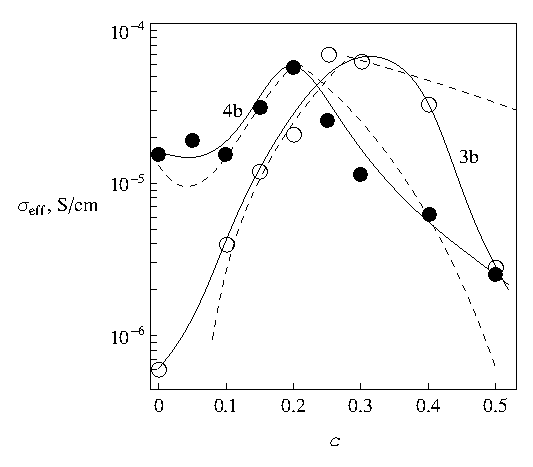
\includegraphics[width=0.5\textwidth]{Fig5_Comparison.eps}
	\caption{\label{fig:comparison_polymer} Порівняння результатів
		моделі тришарової оболонки (неперервні лінії 3b та 4b, див.
		таблиці~\ref{tab:adjustable_params-21}, \ref{tab:adjustable_params-22}) з модифікованою для 
		ПКЕ теорією Накамури Нана Вічорека~\cite{Wiec1994} (штрихована лінія, див. 
		таблицю~7 та рис.~10 у \cite{Wiec1994}) на прикладі обробки
		даних~\cite{Wiec1994} для PEO--LiClO$_4$--PAAM ($\circ$) та
		OMPEO--LiClO$_4$--PAAM (після отжигу) ($\bullet$) при $25 {\rm ^oC}$ 
		%(концентрація LiClO$_4$ дорівнювала 10~mol~\% по відношенню до концентрації ефіру кисню)
	}
\end{figure}

У силу різної фізичної природи задіяних механізмів, параметри різних ділянок ${z}_2(u)$ повинні по-різному залежати від температури. Це припущення відкриває додаткові можливості для подальшого тестування та розширення теорії та досліджується на прикладі температурної залежності ${z}_{\rm eff}$ для ПКЕ $\rm OMPEO-LiClO_4-PAAM$ (після отжигу) \cite{Wiec1994}. 


\subsection{Аналіз температурних залежностей}%\mbox{}

Оскільки три ділянки профілю ${z}_2(u)$ для ПКЕ $\rm OMPEO-LiClO_4-PAAM$ (після отжигу)~\cite{Wiec1994} та фаза матриці формуються процесами в областях з різними ступенями аморфності, температурну залежність кожного з параметрів ${z}_{2,m}$ та ${z}_0$ цих ділянок можна незалежно моделювати за допомогою трипараметричного емпіричного закону Фогеля-Таммана-Фульхера (ФТФ), який зазвичай застосовується для моделювання температурної залежності провідності аморфізованих систем \cite{sequera2010}:
\begin{equation}\label{eq:VTF}
	\sigma = \frac{A}{\sqrt{T}}\exp{\left( -\frac{B}{T-T_0} \right)},
\end{equation}
де $T$ -- температура середовища; $A$, $B$, $T_0$ -- підгінні параметри закону ФТФ. Вважається, що $A$ пов'язаний з концентрацією носіїв струму та слабко залежить від температури \cite{Ferry1997}, $B$ пов'язаний з енергією сегментарної рухливості полімерних ланцюгів \cite{Hou2004}, $T_0$ -- зазвичай на 50--100 градусів відрізняється від температури скловання полімеру \cite{Wiec1994}.
Ці параметри для провідностей розглядуваних ділянок ${z}_{2,m} (T)$ та матриці ${z}_0 (T)$ знаходяться шляхом обробки трьох ізотерм ${z}_{\rm eff} (c,T)$ в рамках моделі з тришаровим ступінчатим профілем (\ref{eq:profilex2-triple}) при фіксованих значеннях інших параметрів моделі (див. таблицю~\ref{tab:adjustable_params-22}). 
На рис.~\ref{fig:OMPEO-LiClO4-Temp} представлені результати обробки ізотерм ПКЕ $\rm OMPEO-LiClO_4-PAAM$~\cite{Wiec1994} (використані параметри представлені в таблиці~\ref{tab:isotherms}). З рисунку видно, що запропонована теорія (неперервна лінія) дає кращі результати обробки цих ізотерм {\color{violet}(найменше значення $R^2\approx 87.2\%$ отримано для $T=273$~K)}, ніж використання закону ФТФ (\ref{eq:VTF}) для ${z}_{\rm eff}$ на всьому проміжку температур (штрихована лінія), що було запропоновано в \cite{Wiec1994}.

\begin{figure}[tb]
	\centering
	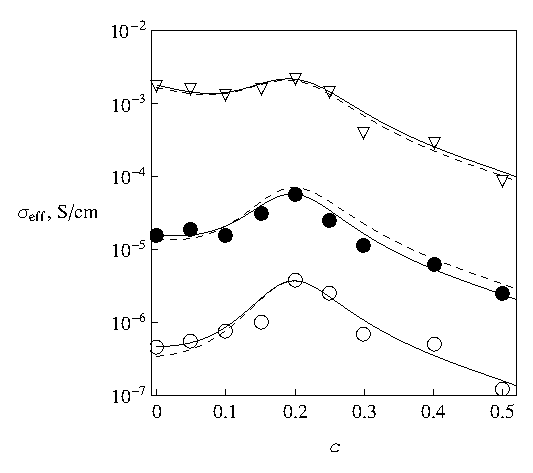
\includegraphics[width=0.55\textwidth]{Fig6_Isochores.eps}
	\caption{\label{fig:OMPEO-LiClO4-Temp} Ізотермічні залежності ефективної провідності $\sigma_{\rm eff}$ від $c$ для ПКЕ OMPEO--LiClO$_4$--PAAM (з молярною концентрацією LiClO$_4$ 10~\%, після отжигу)~\cite{Wiec1994} при $T=273$~K ($\circ$), $298$~K ($\bullet$) та $373$~K ($\nabla$) та їх обробка в рамках закону ФТФ (\ref{eq:VTF})  (штриховані лінії) з параметрами, вказаними в таблиці~5 в роботі \cite{Wiec1994}, та моделі (\ref{eq:general_Contlayer_sigma}) з тришаровим ступінчатим профілем (\ref{eq:profilex2-triple}) з параметрами, вказаними в таблиці~\ref{tab:isotherms} (неперервні лінії)}
\end{figure}

Значення параметрів ФТФ для $\sigma_0$ та $\sigma_{2,m}$ (таблиця~\ref{tab:temp}), розраховані за отриманими з обробки ізотерм даними (таблиця \ref{tab:isotherms}), дозволяють відновити температурні залежності ${z}_{\rm eff}$ з різними фіксованими концентраціями PAAM в усьому дослідженому температурному інтервалі (рис.~\ref{fig:OMPEO-LiClO4-TempDependence}). Всі отримані значення параметрів ФТФ лягають у допустимі границі, вказані у \cite{Wiec1994} для всіх зразків OMPEO--LiClO$_4$--PAAM; з цієї точки зору наші результати узгоджені.
Експериментальні дані для зразків при $c=0.05$, 0.25 та 0.40 (рис.~\ref{fig:OMPEO-LiClO4-TempDependence-a}) достатньо добре відновлюються нашою теорією {\color{violet}(середнє значення $R^2\approx 85.23\%$)}. Дані для зразків при $c=0.10$ та 0.50 відновлюються тільки якісно (неперервні лінії на рис.~\ref{fig:OMPEO-LiClO4-TempDependence-b}); домноживши $\sigma_{\rm eff}$ на сталий множник (0.40 та 0.75, відповідно), можна покращити ці результати (точкові лінії на рис.~\ref{fig:OMPEO-LiClO4-TempDependence-b}). Це може свідчити про прояв поблизу цих концентрації більш тонких ефектів, які теорія не бере до уваги.
Для відновлення цих же даних ${z}_{\rm eff}$ тільки в рамках формули ФТФ (\ref{eq:VTF}), для кожного значення $c$ потрібно знаходити відповідні значення параметрів \cite{Wiec1994}. 


\begin{table}[tb]
	\centering
	\caption{\label{tab:isotherms} Значення провідностей, що були використані для підгонок ізотерм концентраційних залежностей
		$\sigma_{\rm{eff}}$ для ПКЕ OMPEO--LiClO$_4$--PAAM 
		(рис.~\ref{fig:OMPEO-LiClO4-Temp}). }
	\begin{threeparttable}
		\begin{tabularx}{\textwidth}{|X|l|l|l|}
			\hline
			\textrm{Складова}   & $T = 273\,\rm {K}$ & $T = 298\, \rm {K}$ & $T = 373\, \rm {K}$ \\
			\hline
			Матриця, $\sigma_0$ \tnote{a}, См/см          &  $4.64\times 10^{-7}$  &  $1.57\times 10^{-5}$  &  $1.78\times 10^{-3}$   \\
			Перша оболонка, $\sigma_{21}$, См/см   &  $5.75\times 10^{-7}$  &  $8.70\times 10^{-6}$  &  $4.21\times 10^{-4}$    \\
			Друга оболонка, $\sigma_{22}$, См/см  &  $1.025\times 10^{-3}$ &  $7.74\times 10^{-3}$  &  $1.00\times 10^{-1}$   \\
			Третя оболонка, $\sigma_{23}$, См/см   &  $1.07\times 10^{-7}$  &  $3.12\times 10^{-6}$  &  $1.36\times 10^{-4}$ \\
			\hline
		\end{tabularx}
		\begin{tablenotes}
			\item[a] З молярною долею LiClO$_4$ 10 \%. 
		\end{tablenotes}
	\end{threeparttable}
\end{table}

Зауважимо, що отримані значення параметрів $B\approx 1270$~K та $T_0\approx 190$~K для $\sigma_0$ дуже близькі до оцінок, отриманих в \cite{Wiec1994}, для чистого OMPEO ($B = 1200$~K та $T_0 = 195$~K), однак значення параметру $A\approx 36.1\,$См${\rm \cdot K^{1/2}/}$см помітно відрізняється від отриманого в \cite{Wiec1994}: $A=27.0\,$См${\rm \cdot K^{1/2}/}$см. Це може наслідком залежності електричних властивостей матриці від концентрації PAAM.



\section{Висновки}

Показано, що отримані співвідношення (\ref{eq:general_1layer_sigma}), (\ref{eq:general_Contlayer_sigma}) для статичної ефективної провідності спроможні повністю відтворити дані симуляцій в рамках алгоритму RRN, беручи до уваги  особливості  використаного в симуляціях алгоритму та пов'язані з цим проблеми відображення результатів моделі на дані симуляцій. Це свідчить про послідовність досліджуваної моделі та можливість застосовувати її для аналізу ефективної провідності реальних систем.

Продемонстровано застосовність теорії для обробки експериментальних даних з ефективної квазістатичної провідності ТКЕ $\rm LiI-Al_2O_3$ \cite{Liang1973} та ПКЕ PEO--NaI--NASICON,  (PEO)$_{10}$--NaI--$\theta$Al$_2$O$_3$, PEO--LiClO$_4$--PAAM та OMPEO--LiClO$_4$--PAAM \cite{Przl1995, Wiec1994}. 
%Показано, що отримана структура профілю провідності може ефективно відображати фізико-хімічні ефекти та механізми, присутні у наявній системі.
Зроблено і аргументовано припущення, що отримані за результатами такої обробки профілі провідності оболонок можуть бути використані для аналізу ролі різних фізико-хімічних механізмів у формуванні ефективної провідності  $\sigma_{\rm eff}$.

\begin{figure}[tb]
	\centering
	\begin{subfigure}[c]{0.48\textwidth}
		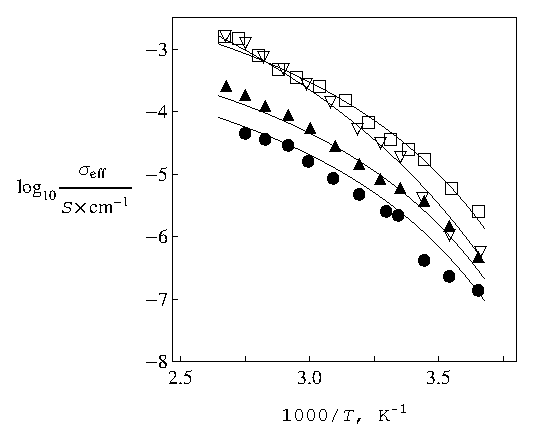
\includegraphics[width=\textwidth]{Fig8_TemperatureDependence_1.eps}
		\caption{} \label{fig:OMPEO-LiClO4-TempDependence-a}
	\end{subfigure}
	\quad
	\begin{subfigure}[c]{0.48\textwidth}
		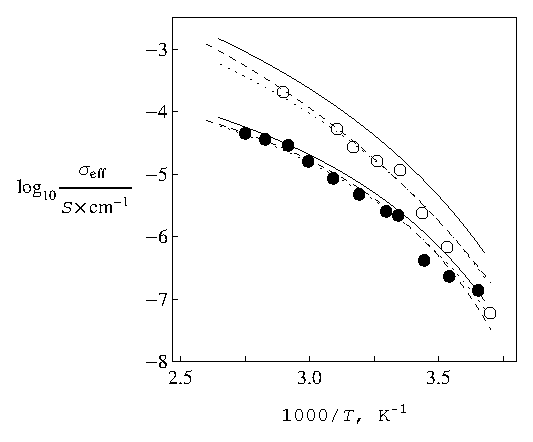
\includegraphics[width=\textwidth]{Fig8_TemperatureDependence_2.eps}
		\caption{} \label{fig:OMPEO-LiClO4-TempDependence-b}
	\end{subfigure}
	\caption{\label{fig:OMPEO-LiClO4-TempDependence}
		Ізохоричні залежності ефективної провідності $\sigma_{\rm eff}$ від $T$ для ПКЕ OMPEO--LiClO$_4$--PAAM (з молярною концентрацією LiClO$_4$ 10~\%, після отжигу)~\cite{Wiec1994} при $c=0.05$ ($\nabla$), 0.10 ($\circ$), 0.25 ($\square$), 0.40 ($\blacktriangle$) та 0.50 ($\bullet$) та їх обробка в рамках тришарової моделі порфілю (\ref{eq:profilex2-triple})  (неперервні лінії), вважаючи, що провідності складових
		підкоряються закону ФТФ (\ref{eq:VTF}) з параметрами, представленими у таблиці~\ref{tab:temp}. Точкові лінії на рис.~(б): те ж саме, але з використанням сталого множнику для $\sigma_{\rm eff}$: $0.40$ та $0.75$ при $c=0.10$ та 0.50, відповідно; штриховані лінії, на рис.~(б): підгонки за формулою ФТФ (\ref{eq:VTF}), використовуючи параметри з таблиці~5 в \cite{Wiec1994}}
\end{figure}



\begin{table}[tb]
	\centering
	\caption{\label{tab:temp} Параметри ФТФ, 
		отримані для ПКЕ OMPEO--LiClO$_4$--PAAM \tnote{a}}
	\begin{threeparttable} 
		\begin{tabular}{|l|l|l|l|}
			\hline
			\textrm{Складова}   & $A$, См$\cdot \rm{K}^{1/2}/$см & $B$, K & $T_0$, K  \\
			\hline
			Матриця \tnote{a}          &  36.1  &  1270  &  190   \\
			Перша оболонка   &  4.33  &  1210   &  180    \\
			Друга оболонка  &  71.1   &  634     &  197   \\
			Третя оболонка   & 0.229   &  720   &  212 \\
			\hline
		\end{tabular}
		\begin{tablenotes}
			\item[a] З молярною долею LiClO$_4$ 10 \%.
		\end{tablenotes}
	\end{threeparttable}
\end{table}

Зокрема, для ТКЕ $\rm LiI-Al_2O_3$ профіль електричної провідності оболонки має дві ділянки. Дальня ділянка відповідає за ефекти, пов'язані зі змінами електричних властивостей матриці у процесі створення зразку в залежності від концентрації дисперсних частинок; ближня частина відображає утворення областей просторового заряду навколо частинок, що підтверджується порівнянням характеристик цих областей з результатами інших авторів \cite{Jiang1995a, Jiang1995b}.

Для досліджуваних ПКЕ результати обробки показують наявність двох-трьох чітко виражених ділянок в отриманих профілях провідності. Центральна ділянка (дальня, у випадку тільки двох ділянок) відображає ефект формування навколо частинок в ПКЕ аморфізованих областей з відносно високою провідністю. 
Найближча до ядер ділянка описує сумарний ефект кількох можливих процесів: ``stiffening effect'' -- ефект затвердіння, що веде до зниження локальної провідності; залежність значення локальної провідності від провідних властивостей частинок, а отже і природи міжфазної поверхні; нерегулярність форми частинок.
Найвіддаленіша ділянка для ПКЕ $\rm OMPEO-LiClO_4-PAAM$ ефективно відображає залежність провідності матриці від $c$, що може бути викликана зв'язуваннями іонами солі поодиноких молекул PAAM, розподілених в матриці поза межами глобул PAAM \cite{Wiec1994}.
%утворенням зв'язків вільних іонів солі з окремими молекулами PAAM, що залишилися поза межами практично  непровідних глобул PAAM \cite{Wiec1994}.

Області, що відповідають різним ділянкам профілю для ПКЕ $\rm OMPEO-LiClO_4-PAAM$, мають різні ступіні аморфності, що дозволяє моделювати температурну залежність провідності кожної з них за емпіричним законом Фогеля-Таммана-Фульхера (ФТФ). Отримані, з обробки трьох ізотерм, параметри ФТФ дозволяють відновити експериментальні дані $\sigma_{\rm eff}$ на всьому досліджуваному інтервалі температур для п'яти різних значень $c$.

Результати розділу представлено в публікаціях \cite{Sushko2018JML, Sushko2018PRE}.


%%%%%%%%%%%%%%%%%%%%%%%%%%%%%%%%%%%%%%%%%%%%%%%
\chapter{Опис електричної перколяції в системах типу ізо\-лятор~-~провідник з міжфазним шаром}\label{sec:simple-composites}
%%%%%%%%%%%%%%%%%%%%%%%%%%%%%%%%%%%%%%%%%%%%%%%

В даному розділі аналізується ефект електричної перколяції в рамках розробленої моделі для  систем типу ізолятор~-~провідник, що складаються зі слабкопровідної матриці та провідних частинок з проникними оболонками, для яких виконується умова $\sigma_0 \ll \sigma_2 \leq \sigma_1$. Зокрема, аналізуються залежності порогу перколяції та перколяційних критичних індексів провідності від характеристик системи та типовий метод знаходження останніх з наявних експериментальних даних. Досліджується вплив електричної неоднорідності профілю провідності оболонки на прикладі експоненціальноспадних профілів. Проводиться порівняння результатів з експериментаьними даними систем на основі KCl з частинками Ag, покритими проникним оксидним шаром.
% та систем на основі парафіну с частинками термографіту, заліза, алюмінію, CuO та Fe2O3. 


\section{Особливості поведінки електричної провідності}

Для зручності подальшого аналізу перейдемо до безрозмірних змінних $x = \sigma_{\rm eff}/\sigma_1$, $x_i = \sigma_i/\sigma_1$ ($i = 0,1,2$) та розглянемо спочатку ефективну провідність для випадку електрично однорідних оболонок (\ref{eq:general_1layer_sigma}): 
\begin{equation}\label{eq:general_1layer_x}
	(1 - \phi(c,\delta)) \frac{x_0 - x}{2x + x_0}
	+ c \frac{1 - x}{2x + 1}
	+ (\phi(c,\delta) - c) \frac{x_2 - x}{2x + x_2} = 0.
\end{equation}

\subsection{Поріг електричної перколяції}\label{sec:perc-analysis-threshold}
Нагадаємо, що положення порогу перколяції $c_{\rm c}$ визначається в системі з непровідною матрицею ($x_0=0$) та провідними компонентами, як мінімальна концентрація $c_{\rm c}$, при якій провідність не дорівнює нулю. Рівняння (\ref{eq:general_1layer_x}) для такої системи має наступні розв'язки: при $c<c_{\rm c}$ розв'язок тривіальний $x = 0$; при $c > c_{\rm c}$ ненульовим фізично послідовним розв'язком є
\begin{equation}\label{eq:general_1layer_x_x00}
\begin{split}
x =& \frac{3}{4} \left[ \left( c - \frac{1}{3} \right) 
+ \left( \phi - c - \frac{1}{3} \right)x_2 + \right. \\
&\left. + \sqrt{\frac{4}{3} \left( \phi - \frac{1}{3} \right)x_2 + \left[ \left( c - \frac{1}{3} \right) + \left( \phi - c  - \frac{1}{3} \right)x_2 \right]^2} \right].
\end{split}
\end{equation}
Зшивка цих розв'язків при $x_2 > 0$ у точці $c=c_{\rm c}$ можлива лише за умови, що
\begin{equation}\label{eq:threshold}
\phi(c_{\rm c}, \delta) = \frac{1}{3}.
\end{equation}
Це співвідношення й визначає положення порогу перколяції $c_{\rm c}$ ефективної провідності $\sigma_{\rm eff}$. Значення $c_{\rm c}$ визначається лише геометрією оболонки та не залежить від її провідності або проникності. Переходячи до границі $x_2 \to 0$ або $\delta \to 0$, отримуємо значення порогу перколяції для системи твердих ядер $c'_{\rm c} = 1/3$, що збігається зі значенням порогу для СМБ.

\begin{figure}[tb]
	\centering
	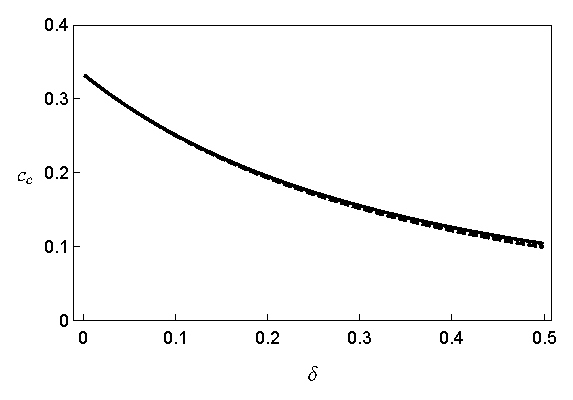
\includegraphics[width=0.6\textwidth]{threshold-delta.eps}
	\caption{\label{fig:threshold-delta}
		Залежність положення порогу перколяції $c_{\rm c}$ від $\delta$ в рамках співвідношення (\ref{eq:threshold}) для функції $\phi$ (\ref{eq:phi_pen}) для системи з проникними оболонками (неперервна лінія) та (\ref{eq:phi-hard}) для системи з твердими оболонками (штрихована лінія)}
\end{figure}

Залежність $c_{\rm c}$ від $\delta$ в рамках співвідношення (\ref{eq:threshold}) для функції $\phi$ (\ref{eq:phi_pen}) частинок з проникними оболонками показана на рис.~\ref{fig:threshold-delta}  (неперервна лінія). Рисунок показує, що для типових значень товщин $\delta \lesssim 0.5$ для знаходження $c_{\rm c}$ може бути використана функція $\phi_t$  (\ref{eq:phi-hard}) для твердих оболонок (штрихована лінія).


\subsection{Ефективні критичні індекси провідності}

За визначенням, перколяційний критичний індекс провідності $t$ вводиться при нульовій провідності матриці ($x_0 = 0$). За цієї умови в околі порогу перколяції при $c > c_{\rm c}$ для ненульових $\delta$, розв'язок (\ref{eq:general_1layer_x_x00}) для $x$  набирає вигляд
\begin{equation}\label{eq:general_1layer_x_x00_cc}
x \approx \frac{3}{4} x_2 \left[ 1 + \frac{\frac{1}{3} + c(1 - x_2)}{\frac{1}{3} - c(1 - x_2)} \right] \left( \phi - \frac{1}{3} \right).
\end{equation}
З цього рівняння видно, що перколяційний критичний індекс $t$ ефективної провідності $\sigma_{\rm eff}$ в рамках моделі дорівнює одиниці. 

Критичний індекс $s$ визначається для систем з ненульовою провідністю матриці ($x_0 \neq 0$), в яких виконується нерівність $x_0\ll x_2, x_1$. 
Якщо при $c<c_{\rm c}$ виконуються нерівності $x\ll x_2\ll 1$, рівняння (\ref{eq:general_1layer_x}) дає наступний розв'язок для $x$ в цій області концентрацій:
\begin{equation}\label{eq:general_1layer_x_x00_cc_s}
x \approx \frac{x_0}{3} \left( \frac{1}{3} - \phi \right)^{-1},
\end{equation}
звідки видно, що індекс $s$ в рамках моделі також дорівнює одиниці.

На практиці, як поріг перколяції $c_{\rm c}$ так і критичні індекси $t$ та $s$ знаходяться шляхом інтерполяції скейлінговими законами (\ref{eq:perc-indexes-s-t}) експериментальних даних з концентраційної залежності провідності, отриманих для деякого інтервалу $c \in [c_1, c_2]$ поблизу $c_c$. При цьому вважається, що коефіцієнт пропорційності в цих законах та самі індекси не залежать від $c$.

Згідно з асимптотиками (\ref{eq:general_1layer_x_x00_cc}) та (\ref{eq:general_1layer_x_x00_cc_s}), коефіцієнти пропорційності для індексів $t$ та $s$ залежать від $c$, а тому зазначені припущення є вірними тільки для дуже вузьких концентраційних інтервалів поблизу $c_{\rm c}$. Таким чином, значення цих індексів, які знаходяться з обробок експериментальних даних, у більшості випадках носять ефективний характер та залежать від інтервалу концентрацій, на якому вони вимірюються (рис.~\ref{fig:teff-seff}):
\begin{subequations}
	\begin{equation} \label{eq:index_teff}
	t_{\rm eff} = {\ln \frac{\sigma_{\rm eff} (c_2)}{\sigma_{\rm eff} (c_1)}}\bigg/{\ln \frac{c_2
			-c_{\rm c}}{c_1 -c_{\rm c}}}; 
	\end{equation}
	\begin{equation} \label{eq:seff}
	s_{\rm eff} = - {\ln \frac{\sigma_{\rm eff} (c_2)}{\sigma_{\rm eff} (c_1)}}\bigg/{\ln
		\frac{c_{\rm c}-c_2}{c_{\rm c}-c_1 }}.
	\end{equation}
\end{subequations}

\begin{figure}[tb]
	\centering
	\begin{subfigure}[b]{0.48\textwidth}
		\begin{overpic}[width=\textwidth]{teff.eps}
			\put(40,55){\small $x_0=0$}
			\dottedline{2}(12.5,13)(12.5,60)
			\dottedline{2}(24.5,13)(24.5,60)
			\dottedline{2}(36.5,13)(36.5,60)
		\end{overpic}
%		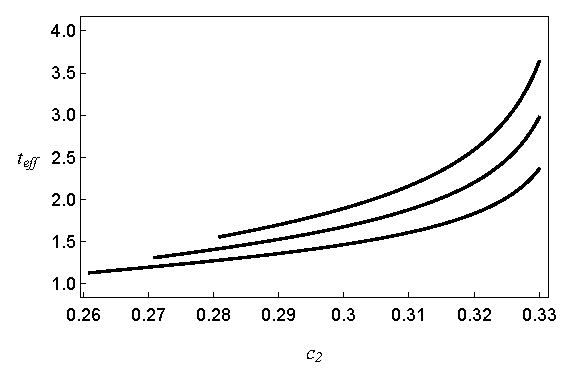
\includegraphics[width=\textwidth]{teff.eps}
		\caption{} \label{fig:teff-seff-a}
	\end{subfigure}
	\quad
	\begin{subfigure}[b]{0.48\textwidth}
		\begin{overpic}[width=\textwidth]{seff.eps}
			\put(20,25){\small $c_1 = 0.24$}
			\put(20,18){\small $c_2 = 0.25$}
		\end{overpic}
%		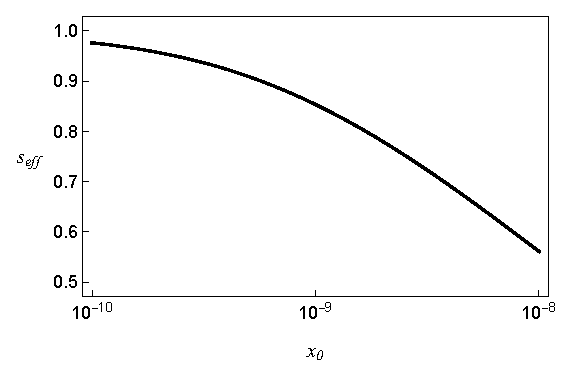
\includegraphics[width=\textwidth]{seff.eps}
		\caption{} \label{fig:teff-seff-b}
	\end{subfigure}
%	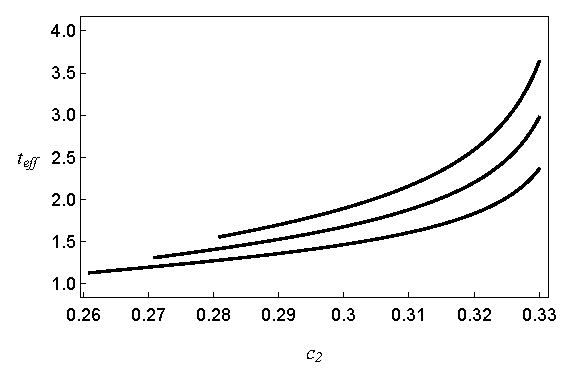
\includegraphics[width=0.6\textwidth]{teff.eps}
	\caption{\label{fig:teff-seff}
	Залежності ефективних критичних індексів: (а) $t_{\rm eff}$ від $c_2$
	при фіксованому $c_1$ та непровідній матриці ($x_0 = 0$); (б)
	$s_{\rm eff}$ від $x_0$ з фіксованими $c_1$ та $c_2$. Вертикальні точкові лінії відповідають значенням $c_1$; $\delta = 0.1$ ($c_c \approx 0.251$) та $x_2 = 5 \times 10^{-5}$}
\end{figure}

%\begin{figure}[!tb]
%	\centering
%	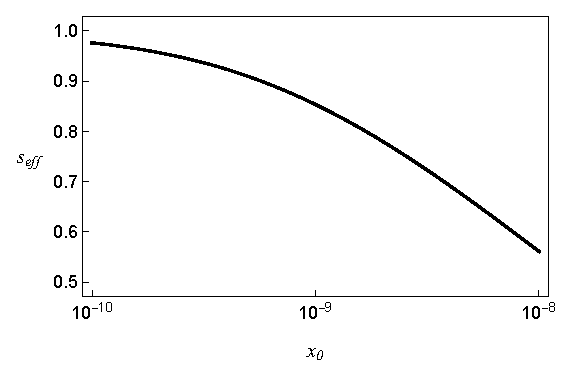
\includegraphics[width=0.6\textwidth]{seff.eps}
%	\caption{\label{fig:seff}
%		Залежність ефективного критичного індексу $s$ 
%		як функція $x_0$ для $\delta = 0.1$ ($c_c \approx 0.251$)
%		та $x_2 = 5 \times 10^{-5}$, розрахована за формулами
%		(\ref{eq:general_1layer_sigma}) та (\ref{eq:seff}) при
%		$c_1 = 0.24$ та $c_2 = 0.25$.}
%\end{figure}

Для фіксованого $\delta \neq 0$, значення індексу $t_{\rm eff}$ зростає з розширенням чи зсувом (при фіксованій ширині) інтервалу $[c_1,c_2]$ при фіксованому значені $c_1$ (рис. \ref{fig:teff-seff-a}). Отримані значення для цього індексу та індексу $s_{\rm eff}$ за (\ref{eq:seff}) та (\ref{eq:general_1layer_x}) (рис. \ref{fig:teff-seff-b}) узгоджуються з їх типовими значеннями (див. розділ~\ref{sec:Bruggeman}). 
Зазначимо, що поріг перколяцій $c_{\rm c}$, знайдений згідно такої процедури, може перевищувати його дійсне значення.


\subsection{Ефект ``подвійної'' перколяції}\label{sec:double-perc}
Для проміжних значень $x_2$ ($x_0 \ll x_2 \ll 1$) можливий ефект подвійної перколяції, що полягає у появі явно виражених двох послідовних перколяційних переходів $x$ (рис.~\ref{fig:percolation}).
Перший з'являється за рахунок утворення перколяційного кластеру з проникних оболонок; другий -- за рахунок прямого контакту більш провідних ядер. Цей ефект може спостерігатися наприклад для рідкокристалічних систем з диспергованими багатостінними нанотрубками \cite{Tomylko2015} або при використанні двокомпонентної матриці \cite{Al-Saleh2008, KonishiY.2006}.

\begin{figure}[tb]
	\centering
	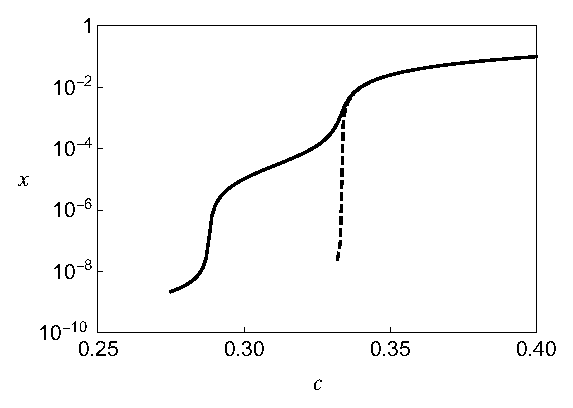
\includegraphics[width=0.6\textwidth]{percolation.eps}
	\caption{\label{fig:percolation}
		Ефекти перколяції (штрихована лінія, $\delta = 0$)
		та ``подвійної'' перколяції (неперервна лінія, $\delta = 0.05$);
		$x_0 = 1 \times 10^{-10}$, $x_2 = 5 \times 10^{-5}$}
\end{figure}

Поріг перколяції $c_{\rm c}$ для першого переходу знаходиться із співвідношення (\ref{eq:threshold}), а критичні індекси дорівнюють одиниці; з урахуванням нерівності $x_2 \ll 1$, положення другого порогу $c_{\rm c}'$ та відповідні критичні індекси знайдемо розклавши в ряд розв'язок (\ref{eq:general_1layer_x_x00}) за $x_2$ з точністю до першого порядку:
\begin{equation}\label{eq:general_1layer_x_x00-double}
\begin{split}
x \approx \frac{3}{2} \left(c - \frac{1}{3}\right) + \frac{3}{2}\left[ \left( \phi - c - \frac{1}{3} \right) + \frac{1}{3} \frac{\phi-1/3}{c-1/3} \right] x_2.
\end{split}
\end{equation}
Для концентрацій $c > c_{\rm c}'$ виконується $x\gg x_2$, тому домінуючим в (\ref{eq:general_1layer_x_x00-double}) буде перший доданок. Таким чином, поріг для другого перколяційного переходу дорівнює $c_{\rm c}'=1/3$, а критичний індекс $t=1$. Для $c<c_{\rm c}'$ виконується $x \sim x_2$ та при наближенні до $c_{\rm c}'$ домінуючим буде другий доданок у квадратних дужках, тож $s=1$. 


\subsection{Випадок електрично неоднорідних оболонок}

Для знаходження порогу перколяції $c_{\rm c}$ для модельної системи з електрично неоднорідним профілем, розглянемо рівняння (\ref{eq:general_Contlayer_sigma}) у зазначених безрозмірних змінних:
\begin{equation}\label{eq:general_Contlayer_x}
(1 - \phi(c,\delta_M)) \frac{x_0 - x}{2x + x_0}
+ c \frac{1 - x}{2x + 1}
+ \int\limits_0^{\delta_M} \frac{\partial \phi(c,u)}{\partial u} \frac{x_2 (u) - x}{2x + x_2 (u)} du = 0
\end{equation}
для системи з непровідною матрицею ($x_0 = 0$). Фізичний розв'язок такого рівняння, знову ж таки, складається з двох віток, що відповідають наступним концентраційним інтервалам: 1) при $c < c_{\rm c}$ розв'язок тривіальний $x=0$; 2) при $c > c_{\rm c}$ ненульова відносна ефективна провідність $x$ знаходиться із співвідношення:
\begin{equation}\label{eq:general_Contlayer_x_x00}
-\frac{1}{2}(1 - \phi(c,\delta_M)) 
+ c \frac{1 - x}{2x + 1}
+ \int\limits_0^{\delta_M} \frac{\partial \phi(c,u)}{\partial u} \frac{x_2 (u) - x}{2x + x_2 (u)} du = 0.
\end{equation}
Виходячи з умови неперервного зшивання цих двох віток у точці $c_{\rm c}$, для знаходження положення останньої достатньо покласти у (\ref{eq:general_Contlayer_x_x00}) $x=0$ та $c=c_{\rm c}$:
\begin{equation}\label{eq:general_Contlayer_x_x00-sew}
-\frac{1}{2}(1 - \phi(c_{\rm c},\delta_M)) 
+ c_{\rm c}
+ \int\limits_0^{\delta_M} \frac{\partial \phi(c_{\rm c},u)}{\partial u} du = 0,
\end{equation}
що дає рівняння (\ref{eq:threshold}) для знаходження $c_{\rm c}$.
Цей результат підкреслює, що поріг перколяції не залежить від величини і розподілу провідності міжфазних шарів, а визначається лише їх лінійним розміром.

Аналіз критичних індексів будемо проводити на прикладі профілю провідності оболонок виду:
\begin{equation}\label{eq:profile-perc}
\sigma_2 (u) = \sigma_{\rm max} \exp \left[-\left( \frac{u}{\delta} \right)^p \ln\left(\frac{\sigma_{\rm max}}{\sigma_{\rm min}} \right) \right]
\end{equation}
при різних значеннях степеня $p\geq 1$; $\sigma_{\rm max}$ та $\sigma_{\rm min}$ -- значення провідності оболонки при $u=0$
та $u=\delta$, відповідно.
\begin{figure}[!htb]
	\centering
	\begin{subfigure}[c]{0.47\textwidth}
		\begin{overpic}[width=\textwidth]{teff3-thick.eps}
			\put(23,55){\small $x_0=0$}
		\end{overpic}
		\caption{\small $\sigma_{\rm min} = 10^{-10}\sigma_1$} 
		\label{fig:teff3-seff3-a}
	\end{subfigure}%
	\quad
	\begin{subfigure}[c]{0.49\textwidth}
		\begin{overpic}[width=\textwidth]{seff3-thick.eps}
			\put(20,25){\small $c_1 = 0.24$}
			\put(20,18){\small $c_2 = 0.25$}
		\end{overpic}
		\caption{\small $\sigma_{\rm min} = 5\times 10^{-5}\sigma_1$} \label{fig:teff3-seff3-b}
	\end{subfigure}%
	%\vspace{-10pt}
	\caption{\label{fig:teff3-seff3}
		Залежності ефективних критичних індексів: (а) $t_{\rm eff}$ від $c_2$
		при фіксованому $c_1$ та непровідній матриці; (б)
		$s_{\rm eff}$ від $x_0$ з фіксованими $c_1$ та $c_2$. Штрих-пунктирні лінії -- дані для електрично однорідного профілю при $\sigma_2/\sigma_1 = 5 \times 10^{-5}$; неперервні та штриховані лінії -- результати для профілю (\ref{eq:profile-perc}) при, відповідно, $p=1$ та $p=2$, $\sigma_{\rm max} = \sigma_1$. Вертикальні точкові лінії відповідають значенням $c_1$; $\delta = 0.1$ ($c_c \approx 0.251$)}
\end{figure}
Цей профіль при аналізі
індексу $t_{\rm eff}$ (див. рис. \ref{fig:teff3-seff3-a}) розглядався при $\sigma_{\rm min} = 10^{-10}\sigma_1$, $\sigma_{\rm max} = \sigma_1$ для двох значень $p=1$ та $p=2$ (неперервна та штрихована лінії, відповідно). Цей індекс, за визначенням, вводиться при нульовій провідності матриці, тому щоб справджувалася рівність $\sigma_2(\delta)=\sigma_0 = 0$, до профілю додавалось $(-\sigma_{\rm min})$. Індекс $s_{\rm eff}$, за визначенням, вводиться для систем з $x_0 \ll x_2$ та $x_0 \ll 1$, тому значення параметрів профілю (\ref{eq:profile-perc}) були $\sigma_{\rm min} = 10^{-5}\sigma_1$, $\sigma_{\rm max} = \sigma_1$ для значень $p=1$ та $p=2$, при зміні $x_0$ від $10^{-10}$ до $10^{-8}$. 
У порівнянні із залежністю для однорідної оболонки (штрих-пунктирні лінії), залежність $t_{\rm eff}$ для профілю
(\ref{eq:profile-perc}) має більший кут нахилу, що зростає при збільшенні значення $p$ та дозволяє
покрити більшу область значень на фіксованому концентраційному інтервалі  (рис. \ref{fig:teff3-seff3-a}).
Для $s_{\rm eff}$ (рис. \ref{fig:teff3-seff3-b}) якісна
поведінка теж зберігається; змінюється лише область його значень. 


\section{Поведінка ефективної квазістатичної  проникності}

Згідно з рівнянням (\ref{eq:general_1layer_eps}) ефективна проникність у безрозмірних змінних $y = \varepsilon_{\rm eff}/\varepsilon_0$, $y_i = \varepsilon_i/\varepsilon_0$ розраховується наступним чином:
\begin{equation} \label{eq:general_1layer_y}
y =x \frac{(1-\phi)\, \cfrac{(2x+1)^2}{(2x+x_0)^2}\,y_0 +
	c\, y_1 +(\phi-c)\cfrac{(2x+1)^2}{(2x+x_2)^2}\,y_2}{(1-\phi) \cfrac{(2x+1)^2}{(2x+x_0)^2}\, x_0
	+ c +(\phi -c)\cfrac{(2x+1)^2}{(2x+x_2)^2}\, x_2}.
\end{equation}
Для розглядуваних систем можливі наступні чотири випадки поведінки $y$ поблизу порогу перколяції за умови $x \ll 1$.
\begin{enumerate}
	\item Система знаходиться вище порогу перколяції ($c > c_{\rm c}$) та виконуються нерівності $x \gg \sqrt{x_0}$, $x < x_2$ (тобто $\sigma_{\rm eff} \gg \sqrt{\sigma_0 \sigma_1}$, $\sigma_{\rm eff} < \sigma_2$).
	При $x_0 = 0$ ефективна проникність $y$ при наближенні $c$ до $c_{\rm c}$ зверху ($c > c_{\rm c}$) аномально росте:
	\begin{equation}\label{eq:general_1layer_y_x00_cc}
	y \approx x\,
	\frac{(1-\phi)\, \cfrac{1}{4x^2}\,y_0 +
		c\, y_1 +(\phi-c)\cfrac{1}{(2x+x_2)^2}\,y_2}{c +(\phi -c)\cfrac{1}{(2x+x_2)^2}\, x_2} \sim \frac{1}{x} \sim (c - c_{\rm c})^{-t},
	\end{equation}
	що відповідає наведеним у \cite{Efros1976} аргументам. 
	При $x_0 \neq 0$ перший доданок чисельника (\ref{eq:general_1layer_y}) стає аналітичним в точці $c=c_{\rm c}$, а максимальне значення $y$ -- обмеженим 
	зверху та спадає з ростом $x_0$ (рис.~\ref{fig:y_x0}).
	\begin{figure}[!b]
		\centering
		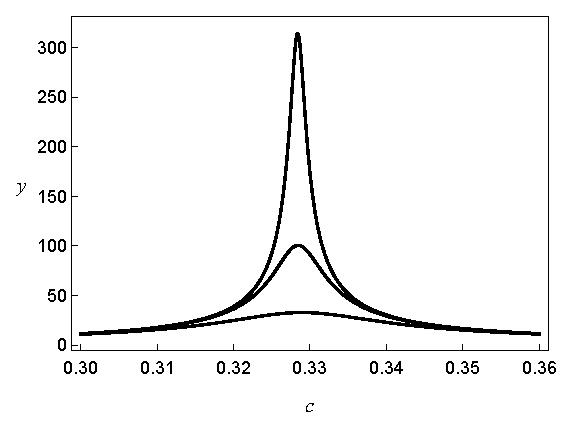
\includegraphics[width=0.6\textwidth]{percolation-eps-x0.eps}
		\caption{\label{fig:y_x0}
			Вплив провідності матриці на ефективну провідність.
			Згори донизу, $x_0 = 1 \times 10^{-6}$, $1 \times 10^{-5}$,
			та $1 \times 10^{-4}$. Інші параметри: $y_1 = 1.5$,
			$y_2 = 1$, $x_2 = 0.05$, $\delta = 0.005$}
	\end{figure} 
	Положення
	максимуму зсувається до менших концентрацій з ростом $\delta$
	(рис.~\ref{fig:y_delta}). Через те, що положення порогу перколяції обумовлене лише геометричними характеристиками структури системи (див. рівняння (\ref{eq:threshold})), положення максимуму $y$ не буде залежати від електричних характеристик компонент.
	
	\begin{figure}[tb]
		\centering
		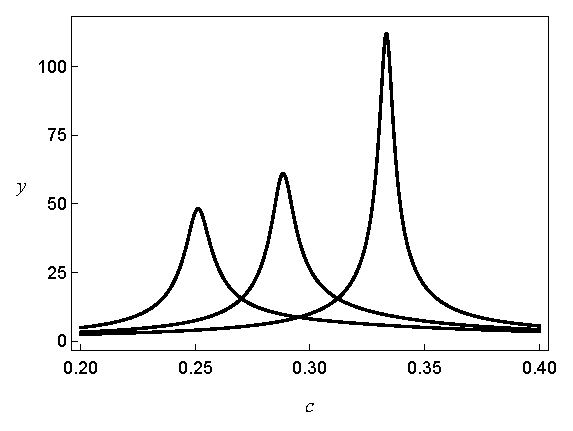
\includegraphics[width=0.6\textwidth]{percolation-eps-d.eps}
		\caption{\label{fig:y_delta}
			Вплив товщини оболонки на ефективну провідність.
			Справа наліво, $\delta = 0$, $0.05$ та $0.10$. 
			Інші параметри: $y_1 = 1.5$, $y_2 = 1$, 
			$x_0 = 1 \times 10^{-5}$, $x_2 = 0.05$}
	\end{figure}

	\item Система знаходиться вище порогу перколяції $c'_{\rm c}$ ($c \geq 1/3$) та виконуються нерівності $x \gg \sqrt{x_0}$, $x \gg \sqrt{x_2}$, $x\gg x_2$ (тобто $\sigma_{\rm eff} \gg \sqrt{\sigma_0 \sigma_1}$, $\sigma_{\rm eff} \gg \sqrt{\sigma_1\sigma_2}$, $\sigma_{\rm eff} \gg \sigma_2$). У даному випадку, домінуючими є перший та третій доданки в чисельнику та другий внесок у знаменнику в (\ref{eq:general_1layer_y}):
	\begin{equation} \label{eq:general_1layer_y-t}
	y \approx x \left[ \frac{(1-\phi)}{c}\, \cfrac{1}{4x^2}\,y_0 +\frac{(\phi-c)}{c}\cfrac{1}{4x^2}\,y_2 \right] \sim \frac{1}{x} \sim (c - 1/3)^{-t}.
	\end{equation}
	
	\item Система знаходиться нижче порогу перколяції ($c<c_{\rm c}$) за умов $x \ll \sqrt{x_0}$, $x \ll \sqrt{x_0 x_2}$, $x \ll x_2$
	(тобто $\sigma_{\rm eff} \ll \sqrt{\sigma_0 \sigma_1}$,
	$\sigma_{\rm eff} \ll \sqrt{\sigma_0 \sigma_2}$ та $\sigma_{\rm eff} \ll \sigma_2$). Тепер домінуючими є перші доданки в чисельнику та знаменнику:
	\begin{equation} \label{eq:general_1layer_y-s}
	y \approx x \frac{(1-\phi)\, \cfrac{1}{(2x+x_0)^2}\,y_0}{(1-\phi) \cfrac{1}{(2x+x_0)^2}\, x_0} \sim x \sim (c_{\rm c} - c)^{-s}.
	\end{equation}
	Критичні індекси у цій та попередній залежностях $y$ не 
	залежать від проникностей $y_i$ компонентів системи та дорівнюють одиниці.
	
	\item Система знаходиться в околі порогу перколяції та $x \gg \sqrt{x_0}$ та $x \gg x_2$ ($\sigma_{\rm eff} \gg 
	\sqrt{\sigma_0 \sigma_1}$, $\sigma_{\rm eff} \gg \sigma_2$).
	Тоді чисельник майже не залежить від $x$, а у знаменнику домінуючими є перший та третій доданки, тож очікується, що проникність веде себе як $y = ax/(1+bx^2)$, де коефіцієнти $a$, $b$ легко знайти з (\ref{eq:general_1layer_y}).
%	залежить від $x^{-2}$, в той час як
%	найголовнішими є другий та третій доданки у знаменнику:
%	\begin{equation} \label{eq:general_1layer_y-cc}
%	y \approx x \frac{(1-\phi)\, \cfrac{1}{4x^2}\,y_0 +
%		c\, y_1 +(\phi-c)\cfrac{1}{x_2^2}\,y_2}{c +(\phi -c)\cfrac{1}{x_2}} \sim a x + \frac{b}{x},
%	\end{equation}
%	де коефіцієнти $a$ та $b$ залежать від $c$:
%	$$
%	a = \frac{cy_1x_2 + (\phi - c)y_2/x_2}{cx_2 + (\phi - c)};
%	\qquad
%	b = \frac{(1-\phi)}{cx_2 + (\phi - c)} \, \frac{y_0}{4x_2}.
%	$$
\end{enumerate}

Якщо порогів перколяції декілька (рис.~\ref{fig:percolation}), то така поведінка проникності виникає поблизу кожного з них (рис.~\ref{fig:double-perc-eps}). 

\begin{figure}[tb]
	\centering
	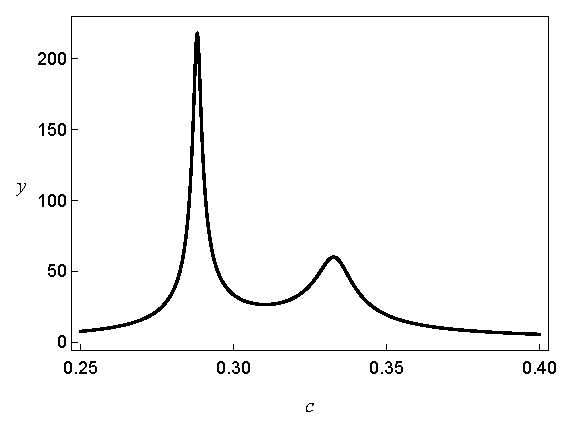
\includegraphics[width=0.6\textwidth]{double-perc-eps.eps}
	\caption{\label{fig:double-perc-eps}
		Ефективна проникність при подвійній перколяції;
		$x_0 = 1 \times 10^{-8}$, $x_2 = 5 \times 10^{-4}$,
		$y_1 = 1.5$, $y_2 = 1$, $\delta = 0.05$}
\end{figure}


\section{Порівняння з експериментальними даними}

%\subsection{Системи KCl-Ag}
В роботах \cite{Grannan1981, ChenI.-G.1986} представлено експериментальні дані з концентраційної залежності ефективних квазістатичних діелектричної проникності та електричної
провідності систем на основі KCl з частинками Ag із середнім радіусом
приблизно 10~нм. Частинки були виготовлені шляхом випаровування Ag у присутності аргону та оксигену задля формування на поверхні частинок тонкої (приблизно 1~нм, $\delta\approx 0.10$) оксидної плівки, що перешкоджала частинкам злипатися, але була достатньо тонка та проникна для виникнення контактів метал~-~метал під великим тиском. Ці частинки додавалися до порошку KCl, перемішувалися та пресувалися під тиском до твердих зразків. Параметри матриці KCl не були визначені в роботі.

\begin{figure}[tb]
	\centering
%	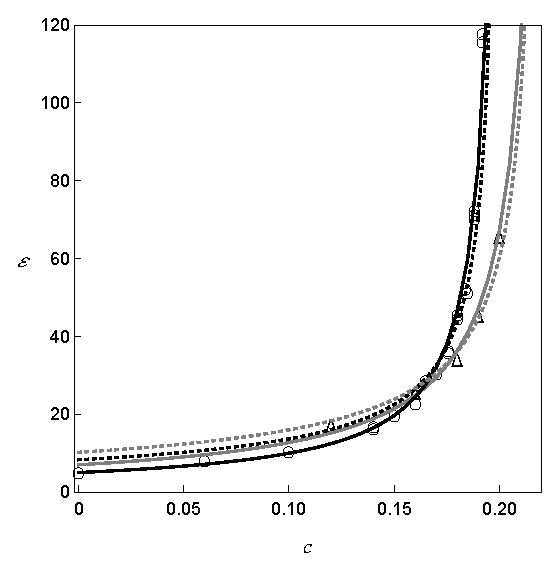
\includegraphics[width=0.55\textwidth]{KCl-Ag-eps.eps}
	\begin{overpic}[width=0.55\textwidth]{chen-grannan-eps.eps}
		\put(19,90){$\circ$ -- $\varepsilon_0 = 5.0$, $\delta = 0.194$,}
		\put(29,83){$s_{\rm eff} = 0.72$}
		\put(17,70){$\triangle$ -- $\varepsilon_0 = 7.0$, $\delta = 0.150$,}
		\put(29,63){$s_{\rm eff} = 0.74$}
		\put(2.5,53){\footnotesize ${\rm eff}$}
	\end{overpic}
\vspace{-5pt}
	\caption{\label{fig:KCl-Ag-eps}
		Залежності ефективної діелектричної проникності $\varepsilon_{\rm eff}$ нанокомпозитів $\rm KCl-Ag$ від концентрації частинок $\rm Ag$ \cite{Grannan1981} та їх обробки за скейлінговими законами  \cite{Grannan1981} для даних при $c > 0.11$ (точкові лінії), та за співвідношенням (\ref{eq:general_1layer_eps}) при $\sigma_0 \approx 3.13 \times 10^{-8}$~См/м, $\sigma_1 \approx 6.25 \times 10^7 $~См/м, $\sigma_2 \approx 250$~См/м (неперервні лінії)}
	\vspace{-5pt}
\end{figure}

На рис.~\ref{fig:KCl-Ag-eps} представлено обробку даних для двох серій експериментальних вимірювань ефективної діелектричної проникності розглядуваних систем при частоті тестуючого поля 1~кГц. Дані були отримані для інтервалу  $c < c_{\rm c}$, на якому внутрішня структура оболонки не проявляється, тому для обробки цих даних достатньо  використовувати модель з однорідною оболонкою (\ref{eq:general_1layer_eps}), яка дає кращі результати ніж скейлінгові закони (точкові лінії). 

Дані для електричної провідності \cite{ChenI.-G.1986} були отримані в околі порогу перколяції, де провідність росте на 7 порядків, у той час як об'ємна концентрація змінюється лише на 1\%. 
На рис.~\ref{fig:KCl-Ag-rhoa} представлено обробку цих даних в рамках моделей (див. рис.~\ref{fig:KCl-Ag-rhob}) з однорідною оболонкою (\ref{eq:general_1layer_sigma}) (штрих-пунктирна лінія) та неоднорідною оболонкою (\ref{eq:general_Contlayer_sigma}) (неперервна лінія) з профілем провідності (\ref{eq:profile-perc}) при $p=3.2$, $\sigma_{\rm max} = \sigma_1$, $\sigma_{\rm min} = 1$~См/м. Значення $\sigma_{\rm min}$ відповідає за порядком величини значенню провідності суміші порошків $\rm AgO$ та $\rm Ag_2O$~\cite{Tvarusko1968}. 

\begin{figure}[tb]
	\centering
	\begin{subfigure}[c]{0.49\textwidth}
		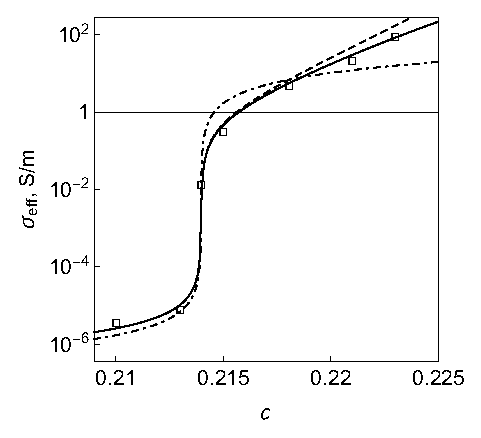
\includegraphics[height=75mm]{chen-grannan-s2-lin.eps}
		\caption{} \label{fig:KCl-Ag-rhoa}
	\end{subfigure}%
	~
	\begin{subfigure}[c]{0.49\textwidth}
		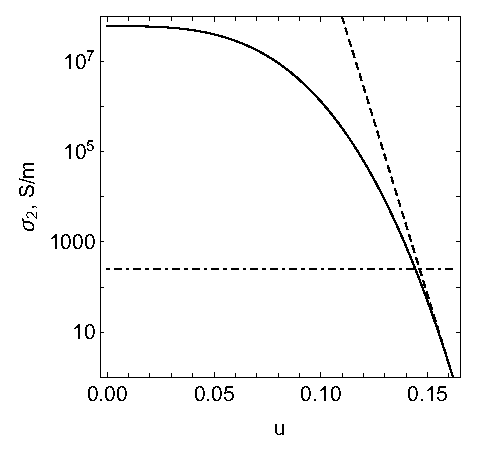
\includegraphics[height=75mm]{chen-grannan-profile-lin-ar1.eps}
		\caption{} \label{fig:KCl-Ag-rhob}
	\end{subfigure}
	\caption{\label{fig:KCl-Ag-rho}
		а) Залежність ефективної провідності систем KCl-Ag \cite{ChenI.-G.1986} від концентрації частинок Ag в околі порогу перколяції та результати її обробки, використовуючи однорідний профіль при $x_2 = 4\times 10^{-6}$, $x_0 = 5 \times 10^{-16}$ (штрих-пунктирна лінія, рис.~б) та неоднорідні профілі (\ref{eq:profile-perc}) та (\ref{eq:profile-perc-exp}) при $p=3.2$, $\sigma_{\rm max} = \sigma_1$, $\sigma_{\rm min} = 1$~См/м, $x_0 = 7.5\times 10^{-16}$ (неперервна та штрихована лінії, відповідно, рис.~б).
		Інші параметри: $\sigma_1 \approx 6.25 \times 10^7 $~См/м, $\delta \approx 0.162$ ($c_{\rm c} \approx 0.214$)}
	\vspace{-10pt}
\end{figure}

Електрично неоднорідна структура профілю може відображати ефект тунелювання електронів, для якого залежність провідності від відстані між двома частинками виражається у вигляді експоненціального закону~\cite{Balberg1987}:
\begin{equation}\label{eq:profile-tunneling}
	\sigma_2 (u) = \sigma_{\rm cont} \exp \left[ - \frac{4u}{\delta_h} \right] ,
\end{equation}
де $\sigma_{\rm cont}$ -- контактна провідність між частинками; $\delta_h = \xi / R_1 $ -- відношення характерної довжини тунелювання $\xi$, що має величину порядку кількох нанометрів, до радіусу ядра частинки. Оцінки значення $\xi$ за знайденими параметрами знаходяться у межах від 0.4 до 1.0 нанометра для значень $\sigma_{\rm cont} = \sigma_1\div 10^{-5}\sigma_1$, відповідно. Як буде показано далі, поблизу точки $u=\delta$ профіль (\ref{eq:profile-perc}) для досліджуваних даних можна досить добре апроксимувати експоненціальним.

Для металевих наночастинок відомим є також так званий spill-out ефект \cite{Weick2006} з характерною товщиною шару spill-out електронів порядку сотих нанометра, що відповідає найближчій до ядра області профілю. Як було показано в розділі \ref{sec:CSE}, різні області профілю мають домінуючу роль на різних інтервалах концентрацій. Зокрема, інтервал, що відповідає найближчій до ядра області, виходить за рамки досліджуваного на експерименті, тож прояв spill-out ефекту в даному випадку не може бути зафіксований за результатами обробки цих експериментальних даних розвинутою теорією. Дійсно, якщо ми обмежимося лінійним членом у розкладі показника експоненти профілю (\ref{eq:profile-perc}) в ряд за $u-\delta$ в околі
$u=\delta$, то отримуємо профіль (див. рис. \ref{fig:KCl-Ag-rhob}, штрихована лінія)
\begin{equation}\label{eq:profile-perc-exp}
	\sigma_2 (u) = \sigma_{\rm min} \exp \left[ - p \ln \left( \frac{\sigma_{\rm max}}{\sigma_{\rm min}} \right) \frac{u - \delta}{\delta} \right] .
\end{equation}
При розрахунку $\sigma_{\rm eff}$ для цього профілю з тими самими параметрами, що були використані для профілю (\ref{eq:profile-perc}), ми отримуємо досить добре узгодження з експериментом (див. рис.~\ref{fig:KCl-Ag-rhoa}, штрихована лінія), яке можна покращити, зменшивши значення $p$. Однак, профіль (\ref{eq:profile-perc-exp}) при малих значеннях $u$ та $p\neq 1$ має асимптотику, відмінну від асимтотики профілю (\ref{eq:profile-perc}).

Ефективні критичні індекси провідності для цих даних можна відновити (див. рис.~\ref{fig:KCl-Ag-rho-loglog}) із залежності логарифму відносної ефективної провідності від логарифму відстані в термінах концентрації від порогу перколяції в областях $c<c_{\rm c}$ та $c > c_{\rm c}$. 
\begin{figure}[tb]
	\centering
	\begin{subfigure}[c]{0.49\textwidth}
		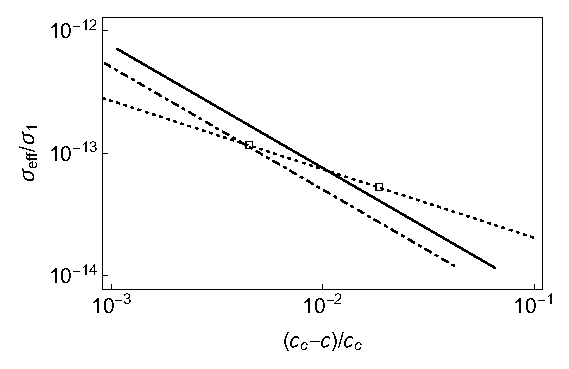
\includegraphics[width=\textwidth]{chen-grannan-s2-loglogs.eps}
		\caption{} \label{fig:KCl-Ag-rho-logloga}
	\end{subfigure}%
	~
	\begin{subfigure}[c]{0.49\textwidth}
		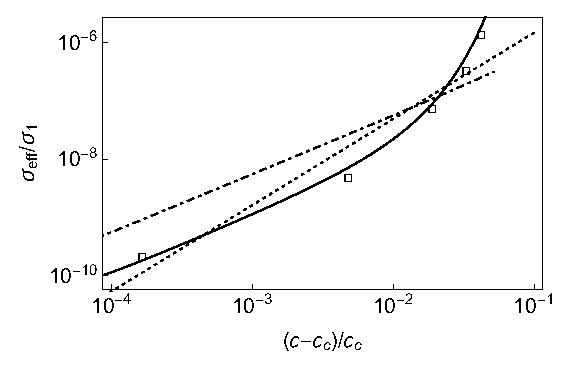
\includegraphics[width=\textwidth]{chen-grannan-s2-loglogt.eps}
		\caption{} \label{fig:KCl-Ag-rho-loglogb}
	\end{subfigure}
	\caption{\label{fig:KCl-Ag-rho-loglog} Залежність (у логарифмічних масштабах) відносної ефективної провідності систем KCl-Ag \cite{ChenI.-G.1986} від відстані до порогу перколяції в областях а) $c < c_{\rm c}$ та б) $c > c_{\rm c}$. Неперервні ($s_{\rm eff} \approx 0.99$, $t_{\rm eff} \approx 1.09 \div 1.60$) та штрих-пунктирні ($s_{\rm eff} \approx 0.68$, $t_{\rm eff} \approx 1.00 \div 1.01$) лінії -- їх обробки, що були представлені на рис.~\ref{fig:KCl-Ag-rho}; точкові лінії -- підгонки методом найменших квадратів ($s_{\rm eff} \approx 0.56$, $t_{\rm eff} \approx 1.48$)}
\end{figure}
Для індексу $s_{\rm eff}$ результат підгонки методом найменших квадратів $s_{\rm eff}\approx 0.56$ та результат для однорідної оболонки $s_{\rm eff} \approx 0.68$ лежать досить близько. Результат для неоднорідного профілю $s_{\rm eff} \approx 0.99$ є близьким до результату моделі ефективного середовища Бруггемана. Для індексу $t_{\rm eff}$ результат методу найменших квадратів $t_{\rm eff} \approx 1.48$ лежить у межах значень, отриманих для неоднорідного профілю, $t_{\rm eff} \approx 1.09 \div 1.60$; однорідний профіль дає результат моделі ефективного середовища $t_{\rm eff} \approx 1.00 \div 1.01$. Всі критичні індекси розраховані для інтервалів $[c_1, c_2]$, де значення концентрацій відповідають експериментальним точкам. Відзначимо, що це лише інтерполяційні оцінки, знайдені для дуже незначної кількості точок.


\section{Висновки}

Показано, що положення порогу перколяції в системах типу ізолятор~-~провідник з міжфазним провідним шаром залежить лише від товщини оболонки.
Теоретично продемонстровано неуніверсальність перколяційних критичних індексів провідності для розглянутих модельних систем \cite{Balberg1987, Myroshnychenko2008} та їх залежність від області, на якій вони вимірюються, та характеру неоднорідності профілю оболонок. Модель передбачає виникнення ефекту подвійної перколяції у системах з проміжним значенням провідності оболонок ($\sigma_0 \ll \sigma_2 \ll \sigma_1$).

Продемонстровано, що неоднорідність профілю провідності оболонок грає суттєву роль у поведінці ефективної провідності дисперсної системи в околі порогу електричної перколяції. За допомогою обробки експериментальних даних можна встановити, щонайменше якісно, структуру цього профілю та дати інтерпретацію його фізичної природи.
Зокрема, в розглянутому нанокомпозиті $\rm KCl-Ag$ неоднорідна структура профілю провідності оксидної оболонки може бути результатом механізму тунелювання електронів, що підтверджується виявленою формою профілю провідності оболонки та оцінками характерної довжини тунелювання. Внески в профіль ефектів, які грають роль при достатньо високих концентраціях (наприклад, spill-out ефект), за цими даними виявити не можливо виявити внаслідок відсутності експериментальних даних для цих концентрацій.

Результати розділу представлено в публікаціях \cite{Sushko2013,Semenov2020}.


%%%%%%%%%%%%%%%%%%%%%%%%%%%%%%%%%%%%%%%%%%%%%%%
\chapter{Критичний аналіз диференціального підходу в рамках МКГ}\label{sec:Hanai-analysis}
%%%%%%%%%%%%%%%%%%%%%%%%%%%%%%%%%%%%%%%%%%%%%%%

В даному розділі МКГ застосовується для критичного аналізу диференціальних схем обчислення ефективної комплексної діелектричної проникності невпорядкованих тривимірних систем на прикладі системи твердих діелектричних куль в діелектричній матриці. Демонструється обмеженість цих схем у квазістатичному наближенні. Для цього, спершу МКГ формулюється у більш зручній формі та показується як рамках останньої можна відновити класичну АМБ. Далі, ця форма використовується для побудови загальних диференціальних рівнянь для діелектричної проникності, з якого знаходяться умови застосування АМБ. Показується, що спроби покращити ці підходи порушують межі Хашина-Штрікмана, що свідчить про їх обмеженість та неможливість  екстраполяції розв'язків диференціальних рівнянь на весь концентраційний інтервал.


\section{Асиметрична модель Бруггемана та диференціальний підхід}\label{sec:Hanai-intro}

Ідею асиметричного моделювання системи можна реалізувати й в рамках підходу ефективного середовища.
Розглянемо систему ${\cal D}_0$ та припустимо, що значення ефективної проникності відомо при деякій концентрації $c$ включень та дорівнює $\varepsilon$. Ставиться задача знайти ефективну проникність $\varepsilon'$ цієї системи після збільшення концентрації частинок на малу величину $\Delta c$ за умови, що $\varepsilon$ змінюється на $\Delta\varepsilon$, а розподіл частинок до та після додавання є рівноважним (див. рис. \ref{fig:HanaiDiff}).
Одним з можливих варіантів розв'язання цієї задачі є асиметрична модель Бругемана (АМБ)~\cite{Bruggeman1935}: вважається, що нова порція частинок (з концентрацією $\Delta c/(1-c)$ у вільній від вже присутніх в системі частинок області) після її додавання може розглядатися окремо на фоні ефективної проникності $\varepsilon$. 
Іншими словами, робиться припущення, що для будь-якого значення $c$ взаємодія між старими частинками та новими може бути замінена взаємодією нових частинок з ефективним середовищем, сформованим старими частинками та матрицею. 
\begin{figure}[tb]
	\centering
	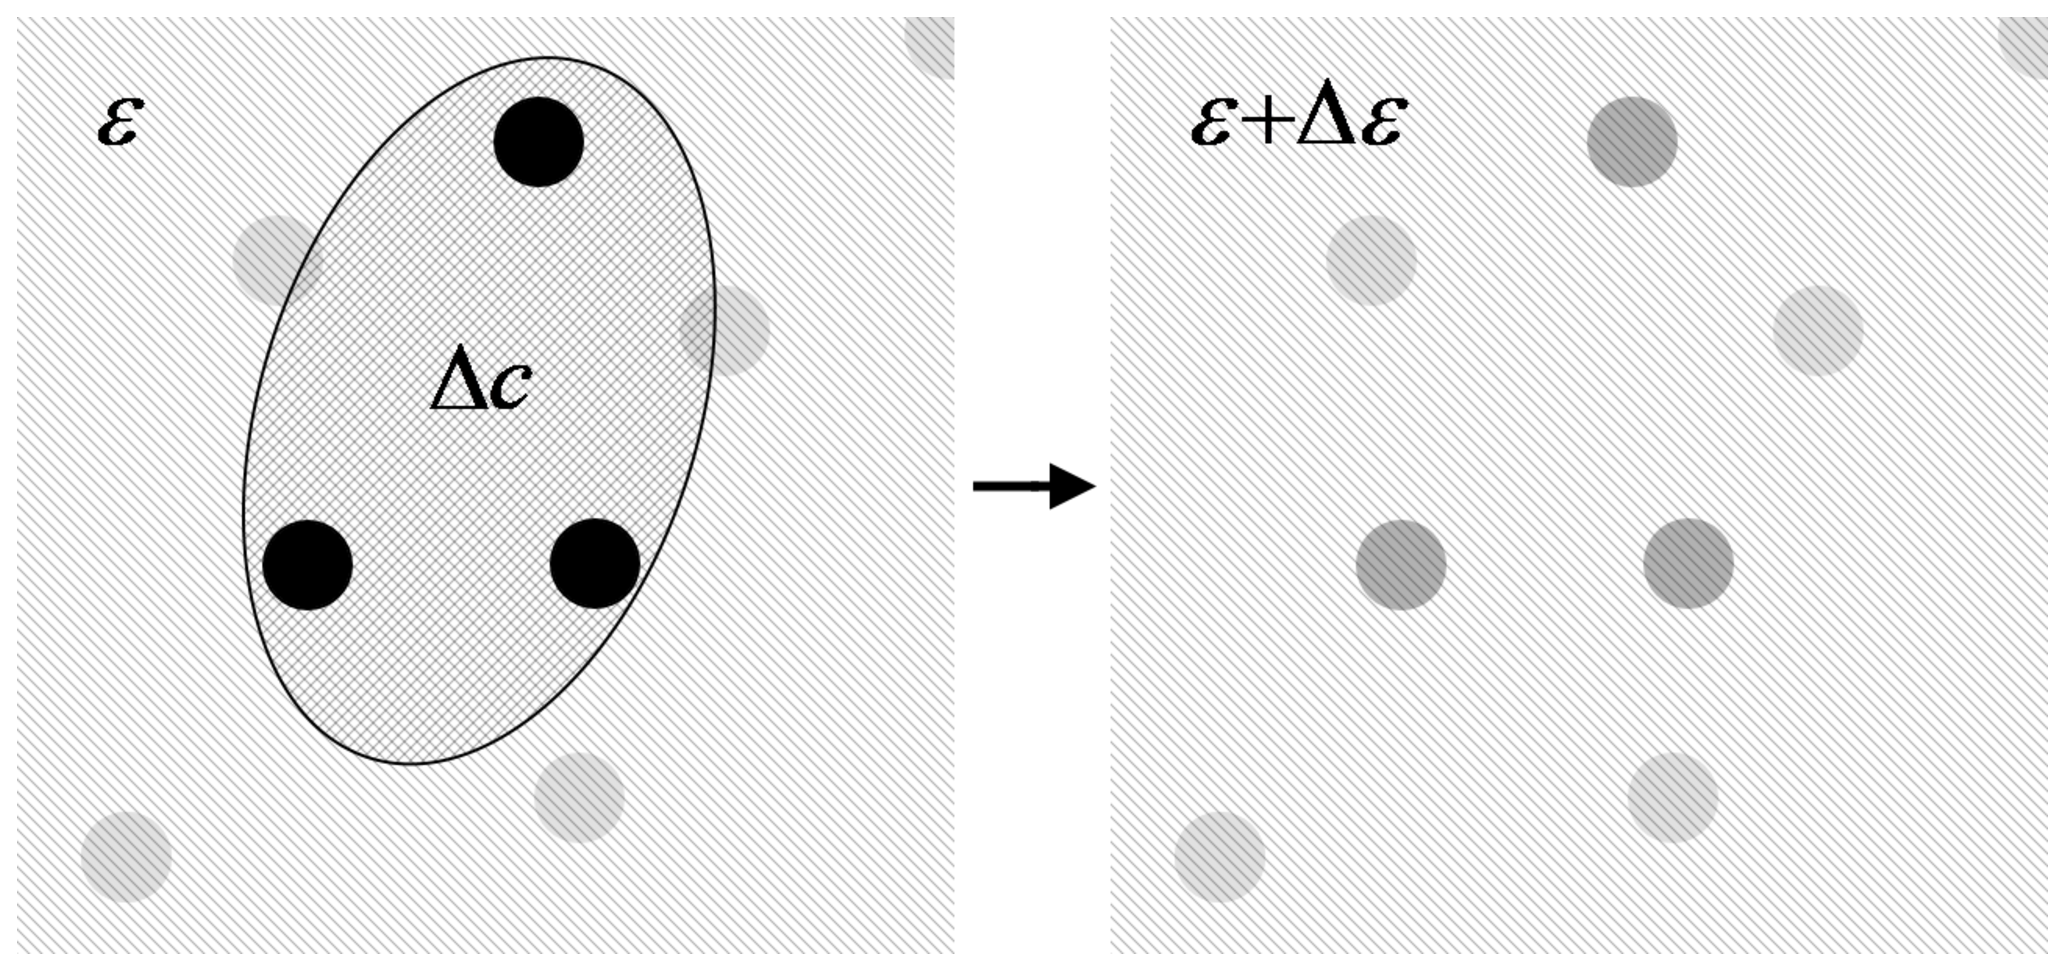
\includegraphics[height=0.3\textwidth]{HanaiDiff.eps}\\
	(а)\qquad\qquad\qquad\qquad\qquad\qquad(б)
	\caption{\label{fig:HanaiDiff}Схематичне представлення
		диференціального алгоритму АМБ: (а) додавання порції
		нових частинок з концентрацією $\Delta c/(1-c)$ у вільній
		від частинок області в дане ефективне середовище з
		проникністю $\varepsilon$ (світліша область) призводить до
		(б) формування нового ефективного середовища з проникністю
		$\varepsilon + \Delta\varepsilon$, що грає роль матриці для
		наступної порції включень. Таким чином, попередні порції
		електрично взаємодіють з новими тільки за рахунок
		ефективного середовища (нові частинки зображені
		темніш{\colr е})}
\end{figure}
Тому, вважаючи концентрацію $\Delta c/(1-c)$ достатньо малою, нову проникність $\varepsilon'$ можна шукати  в рамках підходу МГ (\ref{eq:MG}) для частинок нової порції в матриці з проникністю $\varepsilon$:
\begin{equation}\label{eq:Hanai-diff-start}
\frac{\varepsilon' - \varepsilon}{2 \varepsilon + \varepsilon'} = \frac{\Delta c}{1 - c}\, \frac{\varepsilon_1 - \varepsilon}{2\varepsilon + \varepsilon_1}. 
%= \frac{\Delta\varepsilon}{3 \varepsilon + \Delta\varepsilon}
\end{equation}
Підставляючи в це рівняння $\varepsilon' = \varepsilon + \Delta\varepsilon$, отримуємо рекурсивне співвідношення для знаходження ефективної проникності системи при різних концентраціях частинок.
Числові методи розв'язання цього співвідношення носять назву поступового (``інкрементального'') підходу Максвела-Гарнетта~\cite{Lakhtakia1998, Michel2001}.

Утримуючи лише члени першого порядку  малості за $\Delta c$, $\Delta \varepsilon$ та вважаючи їх нескінченно малими, з  (\ref{eq:Hanai-diff-start}) отримуємо диференціальне рівняння:
\begin{equation}\label{eq:Hanai-diff}
\frac{d c}{1 - c} = \frac{d\varepsilon}{3\varepsilon} \frac{(2\varepsilon+\varepsilon_1)}{(\varepsilon_1 - \varepsilon)},
\end{equation}
що має особливість в точці $c = 1$, а розв'язок в цій точці має задовольняти рівності $\varepsilon = \varepsilon_1$. Співвідношення АМБ для $\varepsilon_{\rm eff}$ отримуємо, інтегруючи ліву частину (\ref{eq:Hanai-diff}) в межах від нуля до $c$ та праву -- від $\varepsilon_0$ до $\varepsilon_{\rm eff}$:
\begin{equation}\label{eq:Hanai}
1 - c = \frac{\varepsilon_{\rm eff} - \varepsilon_1}{\varepsilon_0 - \varepsilon_1} \left( \frac{{ \varepsilon_0}}{\varepsilon_{\rm eff}} \right)^{1/3}.
\end{equation}

Аналогічним чином можна знайти співвідношення АМБ для випадку, коли порції частинок віднімаються, розглядаючи додавання порцій фази матриці, що зменшують кількість частинок~\cite{Sen1981}:
\begin{equation}\label{eq:Hanai-diff-high}
-\frac{d c}{c} = \frac{d\varepsilon}{3\varepsilon} \frac{(2\varepsilon+\varepsilon_0)}{(\varepsilon_0 - \varepsilon)};
\end{equation}
\begin{equation}\label{eq:Hanai-high}
c = \frac{\varepsilon_{\rm eff} - \varepsilon_0}{\varepsilon_1 - \varepsilon_0} \left( \frac{\varepsilon_1}{\varepsilon_{\rm eff}} \right)^{1/3}.
\end{equation}

Узагальнення цього методу для комплексних проникностей носить назву моделі Бруггемана-Ханая або Максвела-Вагнера-Ханая~\cite{Hanai1960, Sen1981}.

Результати АМБ добре застосовні до емульсій типу вода~-~олія/олія~-~вода при частотах тестуючого поля порядку ГГц \cite{Hanai1960}, пористих осадових порід \cite{Sen1981} тощо, диференціальний підхід може бути використаний для отримання й інших відомих результатів, наприклад, поширених в технічній літературі правил Ліхтенекера (\ref{eq:licht-ln}) \cite{Simpkin2010} та підходу Луєнги для двокомпонентних систем з малою різницею провідностей компонентів \cite{Looyenga1965}.
%\begin{equation}\label{eq:looyenga}
%\varepsilon_{\rm eff}^{1/3} = (1-c) \varepsilon_0^{1/3} + c \varepsilon_1^{1/3}.
%\end{equation}
На завершення підкреслимо, що диференціальний  підхід побудовано на базі методу МГ з залученням припущень підходу ефективного середовища Бруггемана, тому слід очікувати, що він має ті ж самі обмеження, що й ці базові підходи. 


\section{Побудова диференціальної схеми в рамках МКГ}

Для того, щоб розвинути диференціальну схему в рамках МКГ, переформулюємо його у більш зручній еквівалентній формі.
Для початку, перейдемо до квазістатичного наближення ($k_0 \to 0$) у виразі для пропагатора (\ref{eq:propagator-eps}):
\begin{equation}\label{eq:prop_longwave_diel}
\lim\limits_{k_0 \to 0} k_0^2 {\widetilde T}_{\alpha \beta} ( {\mathbf{r}} ) = {\widetilde T}_{\alpha \beta}^{(1)} ( {\mathbf{r}} ) + {\widetilde T}_{\alpha \beta}^{(2)}( {\mathbf{r}} ) = \frac{1}{3 \varepsilon_{\rm f}}\delta ({\mathbf{r}}) \delta_{\alpha \beta}
+ \frac{1}{4\pi \varepsilon_{\rm f} r^3} \left( \delta_{\alpha \beta} - 3 \frac{r_{\alpha} r_{\beta}}{r^2} \right)
\end{equation}
та підставимо його до інтегрального рівняння (\ref{eq:integral_field}) для напруженості електричного поля $\bf E$:
\begin{equation}\label{eq:integral_field_SPFT-Tlongwave}
\mathbf{E}(\mathbf{r}) = \mathbf{E}_0(\mathbf{r}) - \frac{\delta\varepsilon({\bf r})}{3 \varepsilon_{\rm f}} \mathbf{E}(\mathbf{r}) - \int\limits_V {d{\mathbf{r}}'}
{\rm{\widetilde T}}^{(2)} (|{\mathbf{r}} - {\mathbf{r}}'|) \delta \varepsilon ({\mathbf{r}}'){\mathbf{E}}({\mathbf{r}}'). 
\end{equation}
Переносячи внесок від дельта-функції (другий доданок в (\ref{eq:integral_field_SPFT-Tlongwave})) у ліву сторону та поділивши обидві частини рівняння на $(1+\delta\varepsilon/3\varepsilon_{\rm f})$,
отримуємо наступне рівняння для $\langle \bf E \rangle$:
\begin{equation}
\langle \mathbf{E} (\mathbf{r}) \rangle = \left\langle \frac{ 3 \varepsilon_{\rm f}  }{3 \varepsilon_{\rm f} + \delta\varepsilon({\bf r})} \right\rangle \mathbf{E}_0
- 3 \varepsilon_{\rm f} \int\limits_V {d{\mathbf{r}}'} { \rm{\widetilde T}}^{(2)} (| {\bf r} - {\bf r}' |)     \left\langle \frac{\delta \varepsilon ({\mathbf{r}}')}{3 \varepsilon_{\rm f} + \delta \varepsilon({\bf r})}{\mathbf{E}}({\mathbf{r}}') \right\rangle  .
\label{eq:wave_prop_int_diel2}
\end{equation}
Для макроскопічно однорідних та ізотропних систем статистичне
середнє під інтегралом залежить лише від $|{\bf r} - {\bf r}'|$,
тож, зважаючи на специфіку кутової частини ${ \rm{\widetilde T}}^{(2)}$,
інтеграл зануляється, а рівняння (\ref{eq:wave_prop_int_diel2})
можна записати наступним чином:
\begin{equation}\label{eq:E_average_diel}
\langle {\bf E} ({\bf r}) \rangle =  \xi {\bf E}_0,\quad
\xi  = \left\langle { \frac{3 \varepsilon_{\rm f}}{3 \varepsilon_{\rm f} + \delta\varepsilon({\bf r})} } \right\rangle.
\end{equation}

Значення середньої індукції поля $\langle \bf D \rangle$ можна знайти з виразу (\ref{eq:eps-eff-def})
\begin{equation}\label{eq:D_average_diel}
\langle {\bf D} ({\bf r}) \rangle = \varepsilon_{\rm f} \eta {\bf E}_0 + \langle \delta\varepsilon ({\bf r}) {\bf E}({\bf r}) \rangle
= \varepsilon_{\rm eff} \langle {\bf E}({\bf r}) \rangle,
\end{equation}
записавши внесок $\langle \delta\varepsilon ({\bf r}) {\bf E}({\bf r}) \rangle$ у явному вигляді, використовуючи такі ж міркування для підінтегрального множнику:
\begin{equation}
\begin{split}
\langle \delta\varepsilon ({\bf r}) {\bf E}({\bf r}) \rangle
=&  \left\langle { \frac{3 \varepsilon_{\rm f} \delta\varepsilon({\bf r})}{3 \varepsilon_{\rm f} + \delta\varepsilon({\bf r})} } \right\rangle {\bf E}_0 - 3 \varepsilon_{\rm f} \int\limits_V {d{\mathbf{r}}'} { \rm{\widetilde T}}^{(2)} (| {\bf r} - {\bf r}' |)     \left\langle \frac{\delta \varepsilon ({\mathbf{r}}) \delta \varepsilon ({\mathbf{r}}')}{3 \varepsilon_{\rm f} + \delta \varepsilon({\bf r})}{\mathbf{E}}({\mathbf{r}}') \right\rangle \\
=& 3 \varepsilon_{\rm f} \eta {\bf E}_0, 
\end{split}
\end{equation}
де було введено позначення
$$
\eta = \left\langle { \frac{ \delta\varepsilon({\bf r})}{3 \varepsilon_{\rm f} + \delta\varepsilon({\bf r})} } \right\rangle.
$$
Використовуючи цей результат та тотожність
\begin{equation}\label{eq:xi-eta_rel}
\xi + \eta \equiv 1,
\end{equation}
остаточно співвідношення (\ref{eq:D_average_diel}) можна переписати у наступному вигляді:
\begin{equation}\label{eq:D_average_diel2}
\langle {\bf D} ({\bf r}) \rangle
= \varepsilon_{\rm f} (1 + 2\xi) {\bf E}_0
= \varepsilon_{\rm eff} \langle {\bf E}({\bf r}) \rangle.
\end{equation}
Зазначимо, що розклавши в ряд $\xi$ та $\eta$
за параметром $(- \delta\varepsilon/3\varepsilon_{\rm f})$
ми отримуємо ітараційні розв'язки МКГ (\ref{eq:ED_average_CGA_origin}).

Підставляючи отримане рівняння (\ref{eq:E_average_diel}) для $\langle {\bf E}({\bf r}) \rangle$ у праву частину рівняння (\ref{eq:D_average_diel2}) для $\langle {\bf D}({\bf r}) \rangle$, з урахуванням тотожності (\ref{eq:xi-eta_rel}), отримуємо
\begin{equation}\label{eq:eps-eff-def-eta1}
\varepsilon_{\rm eff} - \varepsilon_{\rm f}
=(\varepsilon_{\rm eff} +2 \varepsilon_{\rm
	f})\eta.
\end{equation}
Щоб знайти невідоме $\varepsilon_{\rm f}$, аналогічно тому як було зроблено в розділі \ref{sec:eps-f}, користуємося граничними умовами для нормальної компоненти індукції $\bf D$ на межі розділу гомогенізованого середовища $\cal{D}$ та матриці ${\cal M}$:
$$
\varepsilon_{\rm f} {\bf E}_{0n}
= \varepsilon_{\rm eff} \left\langle {\bf E} \right\rangle_n = \varepsilon_{\rm eff} \xi {\bf E}_{0n},
$$
що, з урахуванням (\ref{eq:xi-eta_rel}), дає друге співвідношення між $\varepsilon_{\rm f}$ та $\varepsilon_{\rm eff}$:
\begin{equation}\label{eq:eps-eff-def-eta2}
\varepsilon_{\rm eff} - \varepsilon_{\rm f}
= \varepsilon_{\rm eff}\eta.
\end{equation}
Виділяючи $\eta$ з рівнянь (\ref{eq:eps-eff-def-eta1}) та (\ref{eq:eps-eff-def-eta2}), знаходимо наступне рівняння:
\begin{equation}\label{eq:eps_f_rel_homog}
\eta = \frac{\varepsilon_{\rm eff} - \varepsilon_{\rm f}}{2\varepsilon_{\rm f} + \varepsilon_{\rm eff}} = \frac{\varepsilon_{\rm eff} - \varepsilon_{\rm f}}{\varepsilon_{\rm eff}}.
\end{equation}
Це рівняння має два корені: 1) $\varepsilon_{\rm f} = 0$; 2)
$\varepsilon_{\rm f} = \varepsilon_{\rm eff}$, які збігаються із
зазначеними у розділі~\ref{sec:eps-f}. Тож беручи до уваги другий розв'язок, отримуємо $\eta = 0$, тобто
\begin{equation}\label{eq:general_diff}
\left\langle \frac{\delta\varepsilon({\bf r})}{3\varepsilon_{\rm eff} + \delta\varepsilon({\bf r})} \right\rangle = 0,
\end{equation}
що збігається з результатом (\ref{eq:general-CGA-origin-short}), знайденим використовуючи варіаційний принцип Хашина-Штрікмана~\cite{Sushko2017}.

Для отримання співвідношень АМБ (\ref{eq:Hanai}), (\ref{eq:Hanai-high}) в рамках (\ref{eq:general_diff}) будемо виходити з тих же припущень, що були розглянуті в розділі~\ref{sec:Bruggeman}. Нехай значення ефективної проникності $\varepsilon$ відомо при деякій концентрації включень $c = \langle  \Pi_1 ({\bf r}) \rangle$ ($\Pi_1 ({\bf r})$ -- характеристична функція всіх частинок). При додаванні порції нових включень з концентрацією $\Delta c = \langle \Delta\Pi_1({\bf r}) \rangle$ ($\Delta\Pi_1({\bf r})$ -- характеристична функція порції нових частинок; $\Pi_1 \cdot \Delta\Pi_1 = 0$) до системи (виділена область на рис.~\ref{fig:HanaiDiff}(а)) проникність системи зміниться на $\varepsilon + \Delta\varepsilon$ (рис.~\ref{fig:HanaiDiff}(б)).
До та після додавання розподіл всіх включень в системі є рівноважним. Вважається, що наявне ефективне середовище слугує однорідною матрицею для цієї порції частинок та займає область, вільну від всіх доданих частинок, тобто її характеристична функція дорівнює $(1 - \Pi_1 ({\bf r}) - \Delta\Pi_1({\bf r}))$.
Тоді $\delta\varepsilon$ після додавання можна записати у вигляді:
\begin{align}
\delta\varepsilon_{\rm ABM}^{(l)} ({\bf r}) &= (\varepsilon - (\varepsilon + \Delta\varepsilon)) [ 1 - \Pi_1 ({\bf r}) - \Delta\Pi_1 ({\bf r})]
+ (\varepsilon_1 - (\varepsilon + \Delta\varepsilon)) \Delta\Pi_1({\bf r}) \approx \nonumber\\
&\approx - \Delta\varepsilon [ 1 - \Pi_1 ({\bf r}) ] + (\varepsilon_1 - \varepsilon) \Delta\Pi_1({\bf r}),
\label{eq:delta-Hanai}
\end{align}
де були залишені тільки перші порядки малості за $\Delta \Pi_1$
(у сенсі його середнього значення) та $\Delta \varepsilon$;
$\varepsilon$ в (\ref{eq:general_diff}) також потрібно замінити
на $\varepsilon + \Delta\varepsilon$: 
\begin{equation}\label{eq:general_diff-ABM}
\left\langle \frac{\delta\varepsilon_{\rm ABM}^{(l)} ({\bf r})}{3(\varepsilon + \Delta\varepsilon) + \delta\varepsilon_{\rm ABM}^{(l)} ({\bf r})} \right\rangle = 0.
\end{equation}
Верхній індекс $l$ у (\ref{eq:delta-Hanai}) позначає, що ми працюємо з системою, збільшуючи кількість включень. Підставляючи (\ref{eq:delta-Hanai}) до (\ref{eq:general_diff-ABM}), беручи до уваги умову ортогональності для характеристичних функцій 
$$
(1 - \Pi_1 - \Delta\Pi_1)\cdot\Delta\Pi_1 = 0
$$ 
та ергодичну гіпотезу, статистичне усереднення в (\ref{eq:general_diff-ABM}) може бути розбито на усереднення по областям, що займають матриця та нові частинки:
\begin{align}
&-\left\langle \frac{\Delta\varepsilon [1 - \Pi_1 - \Delta \Pi_1]}{3(\varepsilon + \Delta\varepsilon) + \Delta\varepsilon [1 - \Pi_1 - \Delta \Pi_1]} \right\rangle 
+ \left\langle \frac{(\varepsilon_1 - (\varepsilon + \Delta\varepsilon)) \Delta\Pi_1}{3(\varepsilon + \Delta\varepsilon) + (\varepsilon_1 - (\varepsilon + \Delta\varepsilon)) \Delta\Pi_1} \right\rangle \approx \nonumber\\
&\approx - \frac{\Delta\varepsilon}{3\varepsilon} (1 - c) + \frac{\varepsilon_1 - \varepsilon}{2\varepsilon + \varepsilon_1}\Delta c = 0,
\end{align}
де знову були залишені перші порядки малості за тими ж самими змінними. Переходячи до інфінітезимальних змінних $d\varepsilon$ та $dc$ отримуємо диференціальне рівняння (\ref{eq:Hanai-diff}). 

За такою ж схемою можна отримати рівняння (\ref{eq:Hanai-diff-high}), розглядаючи зменшення кількості включень, як додавання порцій матеріалу матриці. Тепер включення розглядаються в якості ``матриці'', а матриця -- в якості ``включень'' з характеристичною функцією $\Pi_0 = (1 - \Pi_1)$. Порція матриці з характеристичною функцією $\Delta\Pi_0 = - \Delta\Pi_1$ додається до системи замість наявних частинок,  характеристичною функцією яких після додавання є $(1 - \Pi_0 - \Delta\Pi_0)$. Відповідно,
\begin{equation}\label{eq:delta-Hanai-high}
\begin{split}
\delta\varepsilon_{\rm ABM}^{(h)} ({\bf r}) =& (\varepsilon - (\varepsilon + \Delta\varepsilon)) [ 1 - \Pi_1 ({\bf r}) - \Delta\Pi_1 ({\bf r})] +\\
&+ (\varepsilon_1 - (\varepsilon + \Delta\varepsilon)) \Delta\Pi_1({\bf r}) \approx \\
\approx& - [ 1 - \Pi_0 ({\bf r}) ] \Delta \varepsilon + (\varepsilon_0 - \varepsilon) \Delta\Pi_0({\bf r}) =\\
=& - \Pi_1 ({\bf r}) \Delta\varepsilon - (\varepsilon_0 - \varepsilon) \Delta\Pi_1({\bf r}).
\end{split}
\end{equation}
Підставляючи (\ref{eq:delta-Hanai-high}) до (\ref{eq:general_diff-ABM})
та переходячи до нескінченно малих, отримуємо шукане друге диференціальне рівняння АМБ (\ref{eq:Hanai-diff-high}).

Можливість отримати АМБ в рамках МКГ дає змогу побудувати та проаналізувати загальну диференціальну схему вивчення ефективних характеристик невпорядкованих дисперсних систем, аналізуючи при цьому окремі внески АМБ.


%\section{Реалізація диференціальної схеми в рамках МКГ}

%\subsection{Побудова диференціальної схеми в рамках МКГ}

В системі діелектричних куль в діелектричній матриці локальні відхилення діелектричної проникності за рахунок компактної групи в околі точки $\bf r$ визначаються розподілом
\begin{equation}\label{eq:delta-Brug-eps}
\delta{\varepsilon}_{\rm CGA} ({\bf r}) = (\varepsilon_0 - \varepsilon) [1 - \Pi_1 ({\bf r})] + (\varepsilon_1 - \varepsilon) \Pi_1 ({\bf r}),
\end{equation}
де $\varepsilon$ -- ефективна діелектрична проникність, сформована наявними компактними групами при деякій концентрації включень $c = \langle \Pi_1 \rangle$. Припустимо, що інфінітезимальна зміна кількості включень в системі викликають малі зміни їх концентрації $\Delta c = \langle \Delta\Pi_1 \rangle$ та ефективної проникності $\Delta\varepsilon$. Тоді, розподіл (\ref{eq:delta-Brug-eps}) та співвідношення (\ref{eq:general_diff}) набувають наступний вигляд, відповідно:
\begin{equation}\label{eq:delta-Brug-diff0}
\begin{split}
\widetilde{\delta\varepsilon}_{\rm CGA} ({\bf r}) =& (\varepsilon_0 - (\varepsilon + \Delta\varepsilon)) [1 - (\Pi_1 ({\bf r}) + \Delta\Pi_1 ({\bf r}))] +\\
&+ (\varepsilon_1 - (\varepsilon +   \Delta\varepsilon)) [\Pi_1 ({\bf r}) + \Delta\Pi_1 ({\bf r})];
\end{split}
\end{equation}
\begin{equation}\label{eq:general_diff-tilde}
\left\langle \frac{\widetilde{\delta\varepsilon}_{\rm CGA}({\bf r})}{3(\varepsilon + \Delta\varepsilon) + \widetilde{\delta\varepsilon}_{\rm CGA}({\bf r})} \right\rangle = 0.
\end{equation}
Нехтуючи другими порядками малості за $\Delta c$ та $\Delta\varepsilon$, (\ref{eq:delta-Brug-diff0}) можна записати у вигляді суми трьох доданків:
\begin{equation}\label{eq:delta-Brug-diff}
\begin{split}
\widetilde{\delta\varepsilon}_{\rm CGA} ({\bf r}) 
\approx& (\varepsilon_0 - \varepsilon) [1 - \Pi_1 ({\bf r})] - (\varepsilon_0 - \varepsilon)  \Delta\Pi_1 ({\bf r}) -  [1 - \Pi_1 ({\bf r})]\Delta\varepsilon \\
&+ (\varepsilon_1 - \varepsilon) \Pi_1 ({\bf r}) + (\varepsilon_1 - \varepsilon) \Delta\Pi_1 ({\bf r}) -  \Pi_1 ({\bf r}) \Delta\varepsilon = \\
=& \delta\varepsilon_{\rm CGA} ({\bf r}) + \delta\varepsilon_{\rm ABM}^{(l)} ({\bf r}) + \delta\varepsilon_{\rm ABM}^{(h)} ({\bf r}),
\end{split}
\end{equation}
де $\delta\varepsilon_{\rm CGA} ({\bf r})$ -- внесок (\ref{eq:delta-Brug-eps}) заданої компактної групи; $\delta\varepsilon_{\rm ABM}^{(l)} ({\bf r})$ -- внесок (\ref{eq:delta-Hanai}), що враховує вплив нових частинок на $\delta{\varepsilon}_{\rm CGA}$; $\delta\varepsilon_{\rm ABM}^{(h)} ({\bf r})$ -- внесок (\ref{eq:delta-Hanai-high}), що враховує вплив зміни кількості матриці  $\delta\varepsilon_{\rm CGA}$.
Підставляючи (\ref{eq:delta-Brug-diff}) до (\ref{eq:general_diff-tilde}) та переходячи до інфінітезимальних змінних отримуємо наступне диференціальне рівняння:
\begin{equation}\label{eq:Bruggeman-diff-general}
\begin{split}
\left[ d c \frac{\varepsilon_1 - \varepsilon}{2\varepsilon + \varepsilon_1} - (1 - c) \, d\varepsilon \frac{3\varepsilon_0}{(2\varepsilon + \varepsilon_0)^2} \right] -& \\
- \left[  d c \frac{\varepsilon_0 - \varepsilon}{2\varepsilon + \varepsilon_0}
+ c \, d\varepsilon \frac{3\varepsilon_1}{(2\varepsilon + \varepsilon_1)^2} \right] &= 0,
\end{split}
\end{equation}
що є диференціальною формою рівняння (\ref{eq:EMA}). 
%Таку форму запису також можна використовувати для аналізу та отримання нових низько- та високо- концентраційних уточнень класичних АМБ.

Таким чином, в рамках МКГ, зміни $\varepsilon$, що викликані
додаванням малої порції включень, не зводяться лише до внесків $\delta\varepsilon_{\rm ABM}^{(l)}$,
викликаних тільки цими включеннями, як в АМБ, але ще й обумовлені змінами в самій матриці
(внесок $\delta\varepsilon_{\rm ABM}^{(h)}$) та станом системи до додавання даної порції (внесок $\delta\varepsilon_{\rm CGA}$).
Класичні співвідношення AМБ (\ref{eq:Hanai}), (\ref{eq:Hanai-high}) отримуємо, якщо знехтувати внесками $\delta\varepsilon_{\rm ABM}^{(h)}$ та $\delta\varepsilon_{\rm CGA}$ або $\delta\varepsilon_{\rm ABM}^{(l)}$ та $\delta\varepsilon_{\rm CGA}$, відповідно. 
Внеском $\delta\varepsilon_{\rm ABM}^{(h)}$ можна знехтувати, якщо розглядати область достатньо малих концентрацій частинок $c$. Дійсно, якщо значення $c$ на стільки мале, що $c\Delta\varepsilon$ можна вважати величиною другого порядку малості, можна знехтувати першим доданком в (\ref{eq:delta-Hanai-high}); це ж саме припущення гарантує виконання рівності $\varepsilon \approx \varepsilon_0 + O(c)$, що дозволяє знехтувати й другим доданком в (\ref{eq:delta-Hanai-high}).  Зазначимо, що зроблене припущення дозволяє знехтувати обома доданками у другій квадратній дужці в (\ref{eq:Bruggeman-diff-general}) та формально звести його до шуканого (\ref{eq:Hanai-diff}), використовуючи рівність $\varepsilon \approx \varepsilon_0 + O(c)$. Однак це не дозволяє знехтувати внеском $\delta\varepsilon_{\rm CGA}$ частинок до додавання нової порції. Додатково припустивши, що різниця між діелектричними проникностями компонентів $|\varepsilon_0 - \varepsilon_1|$ мала, можна знехтувати другим доданком в виразі (\ref{eq:delta-Brug-eps}) для $\delta\varepsilon_{\rm CGA}$, що робить його величиною порядку $O(c)$. Тобто внесок компактної групи, утвореної частинками до додавання нової порції, стає малою величиною, що разом з рівністю $\varepsilon \approx \varepsilon_0 + O(c)$ узгоджується з припущеннями АМБ (матрицею для нових порцій є поточне ефективне середовище). 
Аналогічні викладки дають такий самий результат й для випадку великих концентрацій, коли можна знехтувати внеском $\delta\varepsilon_{\rm ABM}^{(l)}$. 

Таким чином, співвідношення АМБ (\ref{eq:Hanai}), (\ref{eq:Hanai-high}) мають місце тільки коли концентрація компоненту, що додається, досить мала; самі ж припущення АМБ неповні та можливі лише за умов, що
\begin{enumerate}[label=\arabic*)]
	\item концентрація компоненту, що додається, мала;
	\item різниця між діелектричними проникностями компонентів малі.
\end{enumerate}

Розглядаючи тільки першу умову, ми можемо спробувати уточнити класичні співвідношення АМБ, знехтувавши тільки другою (або першою, для високих концентрацій) квадратною дужкою в (\ref{eq:Bruggeman-diff-general}).

%\subsection{Аналіз результатів}

\section{Модифікації підходу АМБ та їх аналіз}

Спершу розглянемо низькоконцентраційних випадок:
\begin{equation}\label{eq:delta-Brug-diff-low-c}
\widetilde{\delta\varepsilon}_{\rm CGA}^{(l)} \approx \delta\varepsilon_{\rm ABM}^{(l)} + \delta\varepsilon_{\rm CGA},
\end{equation}
та знехтуємо лише другою квадратною дужкою в (\ref{eq:Bruggeman-diff-general}), що дає наступне диференціальне рівняння:
\begin{equation}\label{eq:Bruggeman-diff-low-c}
\frac{d c}{1-c} = d\varepsilon \frac{3\varepsilon_0(2\varepsilon + \varepsilon_1)}{(\varepsilon_1 - \varepsilon) (2\varepsilon + \varepsilon_0)^2}.
\end{equation}
Це рівняння також може бути отримано прямою підстановкою (\ref{eq:delta-Brug-diff-low-c}) до (\ref{eq:general_diff-tilde}).

Аналогічна процедура для висококонцентраційного наближення дає
\begin{equation}\label{eq:delta-Brug-diff-high-c}
\widetilde{\delta\varepsilon}_{\rm CGA}^{(h)} \approx \delta\varepsilon_{\rm ABM}^{(h)} + \delta\varepsilon_{\rm CGA},
\end{equation}
\begin{equation}\label{eq:Bruggeman-diff-high-c}
\frac{d c}{c} = - d\varepsilon \frac{3\varepsilon_1 (2\varepsilon + \varepsilon_0)}{(\varepsilon_0 - \varepsilon) (2\varepsilon + \varepsilon_1)^2}.
\end{equation}

Рівняння (\ref{eq:Bruggeman-diff-low-c}) та (\ref{eq:Bruggeman-diff-high-c}) є покращеними диференціальними рівняннями у тому сенсі, що вони частково враховують взаємодію між частинками нової порції та складовими системи до її додавання, за рахунок вкладу $\delta\varepsilon_{\rm CGA}$. Після інтегрування цих рівнянь отримуємо наступні співвідношення для низько- та високо- концентраційних наближень, відповідно:
\begin{equation}\label{eq:Hanai-new}
\begin{split}
\ln{(1-c)} = \frac{9 \varepsilon_0 \varepsilon_1}{(2\varepsilon_1 + \varepsilon_0)^2} \ln{ \frac{3\varepsilon_0 (\varepsilon_{\rm eff} - \varepsilon_1)}{(\varepsilon_0 - \varepsilon_1) (2\varepsilon_{\rm eff} + \varepsilon_0)} }
- \frac{2(\varepsilon_0 - \varepsilon_1) (\varepsilon_0 - \varepsilon_{\rm eff})}{(2\varepsilon_1 + \varepsilon_0) (2\varepsilon_{\rm eff} + \varepsilon_0)};
\end{split}
\end{equation}
\begin{equation}\label{eq:Hanai-high-new}
\ln{c} = \frac{9 \varepsilon_0 \varepsilon_1}{(2\varepsilon_0 + \varepsilon_1)^2} \ln{ \frac{3\varepsilon_1 (\varepsilon_{\rm eff} - \varepsilon_0)}{(\varepsilon_1 - \varepsilon_0) (2\varepsilon_{\rm eff} + \varepsilon_1)} }
- \frac{2(\varepsilon_1 - \varepsilon_0) (\varepsilon_1 - \varepsilon_{\rm eff})}{(2\varepsilon_0 + \varepsilon_1) (2\varepsilon_{\rm eff} + \varepsilon_1)}.
\end{equation}


%\subsection{Порівняння результатів з межами Хашина-Штрікмана}

В порівнянні зі співвідношеннями АМБ очікується, що отримані рівняння (\ref{eq:Hanai-new}), (\ref{eq:Hanai-high-new}) є більш точними та враховують більшу кількість ефектів. Для перевірки цих результатів, розглянемо верхню та нижню межі Хашина-Штрікмана (\ref{eq:HS-bounds}) для діелектричної проникності розглядуваної системи:
\begin{equation}\label{eq:HS-upper}
\varepsilon^{+} = \varepsilon_1 + \frac{3(1 - c)\varepsilon_1 (\varepsilon_0 - \varepsilon_1)}{3\varepsilon_1 + c
	(\varepsilon_0 - \varepsilon_1)},
\end{equation}
\begin{equation}\label{eq:HS-lower}
\varepsilon^{-} = \varepsilon_0 + \frac{3c\varepsilon_0 (\varepsilon_1 - \varepsilon_0)}{3\varepsilon_0 + (1-c) (\varepsilon_1 - \varepsilon_0)}.
\end{equation}

Легко показати, що рівняння (\ref{eq:Hanai-new}) та (\ref{eq:Hanai-high-new}) не задовільняють цим границям. Дійсно, розглянемо (\ref{eq:Hanai-new}) для випадку $\varepsilon_1 \gg \varepsilon_0$ при концентраціях коли $\varepsilon_{\rm eff} \sim \varepsilon_1$ (при $|\varepsilon_{\rm eff} - \varepsilon_1| \sim \varepsilon_1$): 
\begin{equation}
\begin{split}
\ln{(1-c)} &\approx \frac{9 \varepsilon_0}{4\varepsilon_1} \ln{ \frac{3\varepsilon_0 (\varepsilon_1-\varepsilon_{\rm eff})}{2\varepsilon_{\rm eff} \varepsilon_1} }
- \frac{\varepsilon_1 \varepsilon_{\rm eff} - \varepsilon_0 ( \varepsilon_1 + \varepsilon_{\rm eff})}{2\varepsilon_1 \varepsilon_{\rm eff} + \varepsilon_0 (\varepsilon_{\rm eff} + \varepsilon_1)} \approx - \frac{1}{2}.
\end{split}
\end{equation}
Таким чином, $\varepsilon \to \varepsilon_1$ для $c > (1 - e^{-1/2}) \approx 0.393$, що лежить вище ніж верхня межа (\ref{eq:HS-upper}) для тих самих концентрацій ($\varepsilon^{+}/\varepsilon_1 \approx 0.3$). В області низьких концентрацій (\ref{eq:Hanai-new}) збігається з (\ref{eq:Hanai}) та лежить в рамках зазначених меж. 

Розглядаючи співвідношення (\ref{eq:Hanai-high-new}) для того ж самого випадку при концентраціях коли $\varepsilon_{\rm eff} \sim \varepsilon_0$ аналогічним чином отримуємо:
\begin{equation}
\begin{split}
\ln{c} &\approx \frac{9 \varepsilon_0}{\varepsilon_1} \ln{ \frac{3(\varepsilon_{\rm eff} - \varepsilon_0)}{\varepsilon_1} }
- 2 \approx -2.
\end{split}
\end{equation}
Тобто при $c < e^{-2} \approx 0.135$, маємо $\varepsilon \to \varepsilon_0$, що лежить нижче ніж нижня межа (\ref{eq:HS-lower}) при даній концентрації ($\varepsilon^{-}/\varepsilon_0 \approx 2$).

\begin{figure}[!b]
	\centering
	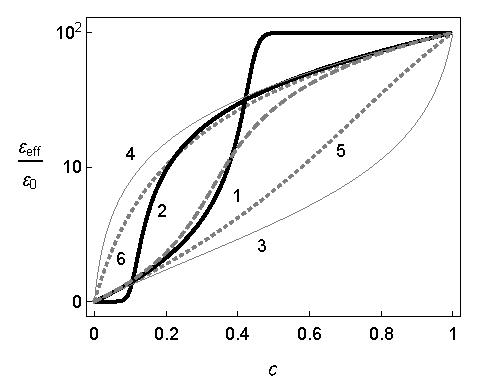
\includegraphics[width=0.6\textwidth]{HSbounds.eps}
	\caption{\label{fig:HS-bounds-check}
		Концентраційні залежності $\varepsilon_{\rm eff}$ згідно
		з: новими низько-~(\ref{eq:Hanai-new}) та високо-~(\ref{eq:Hanai-high-new}) концентраційними законами
		(лінії 1 та 2, відповідно); нижня (\ref{eq:HS-lower})
		та верхня (\ref{eq:HS-upper}) межі Хашина-Штрікмана
		(лінії 3, 4); МКГ (\ref{eq:EMA}) (штрихована лінія);
		класичні низько-~(\ref{eq:Hanai}) та високо-~(\ref{eq:Hanai-high})
		концентраційні підходи АМБ (лінії 5, 6). Було використано значення $\varepsilon_1/\varepsilon_0 = 10^2$}
\end{figure}

Для довільних значень $\varepsilon_1$ та $ \varepsilon_0$ області концентрацій, в яких порушуються межі Хашина-Штрікмана, залежать від відношення $\varepsilon_1/\varepsilon_0$. Рисунок~\ref{fig:HS-bounds-check} демонструє випадок коли $\varepsilon_1/\varepsilon_0 = 10^2$. Помітимо, що оригінальні співвідношення АМБ (\ref{eq:Hanai}) та (\ref{eq:Hanai-high}) задовільняють цим межам. Згідно з вище приведеними аргументами, цей факт ще не означає, що вони кращі ніж їх модифікації (\ref{eq:Hanai-new}) та (\ref{eq:Hanai-high-new}), а лише відображає взаємозв'язок між $ \delta{\varepsilon}_{\rm ABM}^{(l)} ({\bf r})$, $\delta{\varepsilon}_{\rm ABM}^{(h)} ({\bf r})$ та $\delta{\varepsilon}_{\rm CGA} ({\bf r})$, що грає роль в формуванні $\varepsilon_{\rm eff}$ при зміні $c$. Іншими словами, проста екстраполяція уточненого підходу на вузькому концентраційному інтервалі не дозволяє взяти до уваги всі ефекти, що грають роль у формуванні $\varepsilon_{\rm eff}$ при інших концентраціях.

Зазначимо, що наведені результати кількісно підтверджують наявні якісні аргументи~\cite{Chelidze, Chelidze1999} про те, що на високих концентраціях підходи АМБ та Максвелла-Вагнера-Ханая не повністю беруть до уваги міжчастинкові поляризаційні ефекти. Вони також пояснюють чому часто потрібно модифікувати класичні диференційні підходи, або навіть вводити допоміжні підгінні параметри, щоб розширити область застосування моделей~\cite{Becher1987, Sihvola2007}. Також вони задовольняють результатам методу кінцевих елементів \cite{Mejdoubi2007}, який показує, що при малих концентраціях зміни ефективної проникності, викликані додаванням нових порцій частинок, більші ніж ті, що передбачають диференціальні методи.



\section{Висновки}
Аналіз класичної диференціальної схеми, реалізованої в рамках переформульованого МКГ для простих діелектричних макроскопічно однорідних та ізотропних систем в квазістатичному наближенні, показав:
\begin{enumerate}
	\item 
	Класичні диференціальні підходи АМБ можуть бути отримані в рамках МКГ тільки за умови, якщо електродинамічна взаємодія нової порції частинок з вже присутніми заміняється на взаємодію з даним ефективним середовищем. Таким чином, припущення класичних підходів АМБ, в загальному випадку, фізично не послідовні та, строго кажучи, можуть використовуватися лише для розбавлених (відносно однієї з компонент) систем з близькими значеннями їх складових. Співвідношення АМБ можна використовувати для будь-яких розбавлених (відносно однієї з компонент) систем. 
	\item 
	Повна зміна $\varepsilon_{\rm eff}$, викликана додаванням
	інфінітизимальних порцій наповнювача, викликана не тільки внесками змін обох компонентів, а ще й залежить від стану системи перед додаванням. Ігноруючи вклад
	одного з компонентів ми отримуємо узагальнення класичних
	законів АМБ.
	\item 
	Нові узагальнені закони, знову ж таки, можуть бути використані
	тільки на певних концентраційних інтервалах, за межами яких
	порушуються границі Хашина-Штрікмана. Це значить, що за
	формування $\varepsilon_{\rm eff}$ відповідають різні механізми
	на різних концентраційних інтервалах. Просто екстраполяція
	результатів, отриманих на одному з інтервалів, не бере до уваги
	всіх механізмів необхідниих для формування $\varepsilon_{\rm eff}$
	на всьому концентраційному інтервалі.
\end{enumerate}
Отримані результати можуть бути узагальнені на випадок макроскопічно однорідних та ізотропних систем з комплексними проникностями компонентів (беручи до уваги такі ефекти як поляризація Максвела-Вагера).

Результати розділу представлено в публікації \cite{Semenov2018}.


%%%%%%%%%%%%%%%%%%%%%%%%%%%%%%%%%%%%%%%%%%%%%%%
\chapter*{Висновки}
%%%%%%%%%%%%%%%%%%%%%%%%%%%%%%%%%%%%%%%%%%%%%%%

\import{./}{thesis_conclusion-utf8}


%\begin{bibset}{Список використаних джерел}
\bibliographystyle{bibgosts/gost780}
%\bibliographystyle{ugost2003}
%\bibliographystyle{unsrt}%abbrv or plain - alphaeticaly
\bibliography{disser-utf8}
%\end{bibset}


\appendix

%%%%%%%%%%%%%%%%%%%%%%%%%%%%%%%%%%%%%%%%%%%%%%%
\chapter{Список публікацій здобувача та апробація результатів дисертації}
%%%%%%%%%%%%%%%%%%%%%%%%%%%%%%%%%%%%%%%%%%%%%%%

\import{./}{thesis_publications-utf8}


%\label{totalsize}
\end{document}
